\documentclass[british,titlepage, oneside]{project_setup}

\addbibresource{bibliography.bib}


% From https://www.overleaf.com/learn/latex/Glossaries

\makeglossaries % Prepare for adding glossary entries


\newglossaryentry{latex}
{
        name=latex,
        description={Is a mark up language specially suited for
scientific documents}
}

\newglossaryentry{bibliography}
{
        name=bibliography,
        plural=bibliographies,
        description={A list of the books referred to in a scholarly work,
typically printed as an appendix}
}

\newglossaryentry{maths}
{
    name=mathematics,
    description={Mathematics is what mathematicians do}
}


% --------------------
% ----- Acronyms -----
% --------------------

\newacronym{phd}{PhD}{philosophiae doctor}
\newacronym{CoPCSE}{CoPCSE@NTNU}{Community of Practice in Computer ScienceEducation at NTNU}
\newacronym{gcd}{GCD}{Greatest Common Divisor}

\newacronym{ai}{AI}{Artificial Intelligence}


 % add glossary and acronym lists before document

\begin{document}
\setstretch{1.25}

\chapter*{Abstract}

\begin{comment}
A condensation of the essential information of the article.
\end{comment}

In today's increasingly autonomous society, the demand for intelligent, robust solutions are pushing research within guidance, navigation and control to new limits.
In light of its recent advancements, reinforcement learning has established itself as an compelling candidate for the task of guidance and control -- by achieving state-of-the-art performances in robotic tasks. 
Since then, a multitude of algorithms have emerged in this field which has prompted a natural question: how do we decide which algorithm is best for a certain robotic task?
This project aims to serve as a starting point for this question, comparing the characteristics and performances of the two popular reinforcement learning algorithms, Deep Deterministic Policy (DDPG) Gradients and Proximal Policy Optimisation (PPO). 
In this project, these algorithms are trained in a guidance task, commanding accelerations to reach a certain waypoint in 3-dimensional space. Furthermore, models with different hyperparameters combinations are trained and tested, and the results of each analysed. From this, it was discovered that DDPG offered high stability, and by increasing its learning rates and reducing the size of its replay buffer we could improve results. The training of PPO was unexpectedly difficult, where only one model converged to an optimal performance while the rest diverged. The reasons for this are uncertain, though likely caused by too fast learning in the PPO models. Nonetheless, by comparing models relative to a local optimum, it was found that by increasing the batch size, one could then increase the number of optimisation epochs, the number of minibatches and value coefficient to speed up the learning process, while achieving roughly the same average performance. Last, the entropy coefficient was beneficial offering extra exploration. Yet, as the models diverged, these results provide an in-depth understanding of the hyperparameters, but is in no regard a recommendation. Finally, the robustness of the algorithms were tested with a $\pm10\%$ change in mass to the quadrotor. This proved to be an difficult task for the models, where only the best PPO model was able to succeed. Thus, we conclude that the DDPG algorithm is easier to train than PPO, though the potential performance of the PPO algorithm is higher.
%\chapter*{Sammendrag}

Sammendraget skal være \textit{Abstract} på norsk.


\tableofcontents
\listoffigures
\listoftables
%\lstlistoflistings

\printglossary[type=\acronymtype] % Print acronyms
\printglossary                    % Print glossary

\chapter{Introduction}
\label{chap:introduction}

\section{Motivation}

In a world with a heightening level of autonomy, the focus on guidance, navigation and control of robots has never been greater. Likewise, the research community has been in tune with this focus -- innovating, developing and delivering autonomous solutions in novel research domains, ranging from underwater \cite{eelumeSale} to previously unimaginable subterranean environments \cite{washingtonPost}. 
Yet, in light of the increased public interest in autonomy, there comes an increased level of expectation: previous state-of-the-art solutions have now become benchmarks \cite{openAIgym}, and standard environments for robotic applications are alikened to ``pristine conditions'' \cite{washingtonPost}. Also, obtaining funding becomes even more difficult as the bar for what is considered ``new and innovative'' is pushed higher, and potential investors looking for value outcomes are demanding more \cite{reasearchGrant, Gartner}.

Of the vast array of robotic applications and research fields there are, these considerations can provide a motivation for the field of multirotor aerial vehicles (quadrotors). As a result of their low-cost, high versatility, manoeuvrability, relatively simple dynamics and payload potential, multirotor aerial vehicles enable easy exploration of tough environments and a large potential for task customisation. Thus, this field is one that has been gaining momentum in recent years, becoming a standard of aerial robotics research across the world \cite{MultirotorAerialVehicles}.

Next, as expectations for today's robots are raised, so does their anticipated level of autonomy. In terms of its definition, this means that progressively less amount of human operation is expected, with the aim that these systems are able to make informed decisions even when presented with an unexpected event, or while navigating in an unknown environment \cite{TTK23}.
Further, a higher level of autonomy in today's society is linked to the fact that a larger variety of industry and sectors are adopting the use of robotics, while at the same time robotic applications are becoming more complex.

When considering how these dynamical systems will be controlled, we approach a dilemma where the use of classical control theory may be non-ideal. This could be through the difficulty to model or adapt to uncertainties, or through the fact that significant understanding and modelling of a dynamical system is required in order to control it. As the global robotics market is expected to grow at 20.6\% annually for the next five years \cite{roboticsMarket}, it could easily be unsustainable to develop control methods for each individual system, and as such, perhaps alternative control approaches could be considered.

This motivates us to consider the use of learning-based methods, specifically reinforcement learning, which -- through its data-driven approach, high abstraction and evaluative feedback (reward) -- is able to capture both the dynamics of a system and the uncertainties of the environment, to generate complex behaviour without explicit programming \cite{TTK23, RLinRoboticsSurvey}.

\section{Background and Related Work}

The idea of reinforcement learning for robotic applications is not a new one, with previous methods dating back to the 1990s \cite{Gullapalli1994, Miyamoto1996}.
Though only until recently have reinforcement algorithms within this field become unparalleled in performance, setting performance benchmarks in simple Atari games  \cite{mnih2013Atari}, and beating world class players in complex ones such as Dota \cite{ppoOnDota2020}. 
The reason for this success could possibly be accredited to two key moments in reinforcement learning history: first through the successful extension of deep learning to reinforcement learning, to give Deep Q-Networks (DQNs) in 2013 \cite{mnih2013Atari, DQN}, and second, through the extension of DQNs to robotic, reinforcement learning tasks in the continuous domain, to give Deep Deterministic Policy Gradients (DDPG) in 2015 \cite{DDPG}.

Since then, many novel deep reinforcement learning algorithms have been introduced for a wide variety of robotic tasks, such as Trust-Region Policy Optimisation (TRPO) \cite{TRPO}, while just as many others are adapted and ``improved'' versions of previous methods, such as Actor-Critic Experience Replay (ACER) and Proximal Policy Optimisation (PPO) \cite{ACER, PPO}.

In light of these recent advancements, deep reinforcement learning has drawn focus from the cybernetics and control community, leading to a wider use of these methods for guidance and control, 
such as in aerial robotics. For example, deep reinforcement learning is used for autonomous drone landing in \cite{RodriguezRamos2019ADR}, and 3D position control in  \cite{ControlofQuadrotorRL} and \cite{PPOQuadrotor}. Of these, we note the use of three different methods, DDPG, vanilla policy gradient and PPO, respectively. 
Deep reinforcement learning has often been used in navigation tasks as well, ranging from 2D motion planning in \cite{Roy2002MotionPT}, to 3D quadrotor racing using PPO in \cite{song2021droneRacing}. 

Yet, in contrast to the papers that introduce these algorithms \cite{DDPG, PPO}, most of these implementations focus on their own adaptation of an algorithm, including only: a reference to other methods in their background or a simple comparison of their approach against other baseline implementations.

So, with a such a variety of reinforcement learning policies for guidance and control, this begs the question: \textit{how do we really know what the best algorithm is for our control task?} 


\section{Scope}

With the aim of answering this question, this project thesis attempts to compare the best achievable performances of two reinforcement learning algorithms, DDPG and PPO, as a way of attaining a practical understanding of how different aspects of each algorithm and its hyperparameters affect the learning task of quadrotor guidance.

To accomplish this, the project will first compare the effects of hyperparameters in DDPG and PPO separately, analysing the effect these have on the training process and the resulting behaviour of these models in testing. The models are trained to understand how its position and velocity should be mapped to acceleration vectors, in order to reach some waypoint in 3-dimensional space. As for the tests, this will be standardised, such that fair comparisons are made between each model.

The project will compare the some relevant
hyperparameters for each model, but not to the extent of an exhaustive hyperparameter search. Instead, focus will be placed on understanding the effects of each hyperparameter. Finally, the best models for DDPG and PPO, along with their hyperparameter combinations, are compared and discussed.

\section{Outline}

The outline of this project will be as follows:
\vspace{2mm}
\begin{itemize}
    \item \textbf{Chapter 1: Introduction} This chapter includes the motivation for this project, along with reinforcement learning solutions for quadrotor guidance and control.
    \item \textbf{Chapter 2: Theoretical Background} The reinforcement learning problem and its goal is defined in this chapter, presented through the framework of Markov Decision Processes. Last, some considerations are made to illustrate the difficulty of reinforcement learning for robotics.
    \item \textbf{Chapter 3: Policy Optimisation} This chapter presents methods to optimise an agent's policy when it is approximated through parameters. Finally, the DDPG and PPO algorithms are introduced.
    \item \textbf{Chapter 4: Method} This chapter describes the reinforcement learning problem for our quadrotor guidance task. It explains how the experiment is set up and how it is implemented in practice.
    \item \textbf{Chapter 5: Results} The results from training and testing DDPG and PPO are presented in this chapter. This includes training plots, test result tables along with some trajectory plots. In addition, the algorithms' robustness is tested by changing the quadrotor mass by $\pm10\%$.
    \item \textbf{Chapter 6: Discussion} The effects of hyperparameters are discussed, along with any explanations for unexpected or strange results.
    \item \textbf{Chapter 7: Conclusion} The project is concluded by summarising the theoretical differences and results, along with explanations we found for the results.
\end{itemize}























\chapter{Theoretical Background}
\label{chap:background_RL}

\begin{comment}
Background
Fundamentals - MDPs, ValueFunctions
Policy Gradient Methods - Actor-Critc
DDPG
PPO

\begin{itemize}
    \item drone dynamics
    \item MDPs
    \item RL in the continous domain
    \item Policy gradient methods
    \item DDPG
    \item PPO
\end{itemize}
\end{comment}

\section{Overview}

In this section, we will cover the necessary theoretical background required to understand DDPG and PPO. This will start with a gentle introduction to basic RL concepts, including Markov Decision Processes and returns, before moving on to policies and value functions. 

To get an overview of the basics of reinforcement learning, we can begin by looking into its definition and goal. Sutton and Barto \cite{suttonAndBartoBook} states, ``reinforcement learning is learning what to do -- how to map situations to actions -- so as to maximise a numerical reward signal.''
Also, \cite{RLinRoboticsSurvey} states that ``reinforcement learning enables a robot to autonomously discover an optimal behavior through trial-and-error interactions with its environment."

From these, we note a few terms that are worthy of an explanation, such as \textit{situations, actions, rewards, behaviour, trial-and-error interactions} and \textit{environment}.
We can also ask ourselves, ``what exactly is an \textit{optimal} behaviour and how to we express this?''

These concepts are central to reinforcement learning and by the end of this chapter these should be understood. This brings us to the first section, where we will look into Markov Decision Processes.

\section{Finite Markov Decision Processes}
\label{sec:MDPs}

Finite Markov Decision Processes (MDPs) are essentially a standardised learning framework for reinforcement learning. Formally, the MDP framework is comprised of a few elements, often depicted in a diagram as shown in Figure \ref{fig:2_1_simpleMDP}. This diagram depicts an iterative loop: starting first with an initial state, taking an action, observing a new state and reward, then taking the next action and so on.
\begin{figure}[hbt]
    \centering
    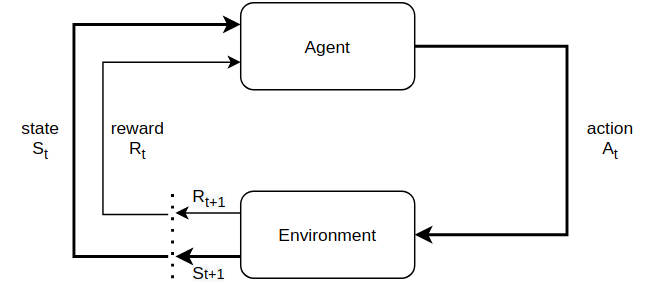
\includegraphics[width=0.8\textwidth]{figures/2_/2_1_simpleEnv2.png}
    \caption{The interaction between agent and environment in an MDP$ $, from \cite{suttonAndBartoBook}.}
    \label{fig:2_1_simpleMDP}
\end{figure}

The first element of an MDP is the \textit{agent}. The agent has the task of \textit{learning} how to solve a specific goal, whereby continuously trying to improve their performance through experience -- or interactions with the \textit{environment}. The \textit{environment} can be thought of as the controlled system, while the agent as the controller.
The situations that an agent finds itself in is referred to as \textit{states} or \textit{observations}. Every state also has the Markov Property, which requires the information in that state only to be dependent on the previous state $S_{t-1}$ and action $A_t$ \cite{suttonAndBartoBook}. 
From a state $S_{t} \in \mathcal{S}$, the agent can take an \textit{action} $A_{t}\in \mathcal{A}$, where $\mathcal{S}$ is the set of states possible and $\mathcal{A}$ is a set of actions for $S_{t}$.
Actions in this case are comparable to control signals and can refer to anything that transitions an agent into a new state such as the acceleration input to a quadrotor or individual torques to rotors. 

An MDP is also includes a \textit{state distribution} $p(s)$ and the states the agent moves to is based on the \textit{state-transition dynamics} $p(s',r|s, a)$, a deterministic function with four arguments that captures the dynamics of the MDP and describes the probability of a specific transition \cite{suttonAndBartoBook}:
\begin{equation}
    p\hspace{0.5mm} (s',r \hspace{0.5mm}|\hspace{0.5mm} s, a) = P \hspace{0.5mm} (S_t = s', \hspace{0.5mm}R_t = r \hspace{0.5mm}|\hspace{0.5mm} S_{t-1} = s,\hspace{0.5mm} A_{t-1} = a )
\end{equation}
Note that $S_t$, $R_t$ and $A_t$ are random variables with well defined probability distributions, while $s$, $r$ and $a$ are particular values of these random variables. The value $s'$ is often a common choice to denote the value of the next state from $s$.

As we can see, the agent receives a numerical \textit{reward} $R_t \in \mathcal{R} \subset \mathbb{R}$ directly from the environment when entering a state $S_t$, which is a sort of evaluative feedback. The reward can be also be function $R(s,a)$ based on the state $s$, action $a$, or also $R(s',a,s)$ which includes the next state $s'$ \cite{TTK23, RLinRoboticsSurvey}. The set $\mathcal{R}$ is used to represent the finite set of rewards possible in an MDP.

To summarise, an MDP can be modelled as the tuple $\langle \mathcal{S},\mathcal{A}, p, R \rangle$, where $\mathcal{S}$ is a finite set of states, $\mathcal{A}$ the finite set of actions for any $S \in \mathcal{S}$, $p$ the state-transition dynamics function $p : \mathcal{S} \times \mathcal{R} \times \mathcal{S} \times \mathcal{A} \rightarrow \mathbb{R} \in [0,1]$  and the reward function $ R : \mathcal{S} \times \mathcal{A} \times \mathcal{S} \rightarrow \mathbb{R}$ \cite{TTK23}.

\section{Returns and Optimal Criteria}
\label{sec:2_ReturnsAndOptimalCriteria}

Now that we have defined MDPs as a framework for learning, we can guess that the agent will try different actions in different states. Eventually, this should allow it to discover an optimal behaviour -- essentially knowing which action is best for each state $s \in \mathcal{S}$. Before, we look into the how to find this behaviour, we will first need to specifically define what we by ``good'' or ``bad'' behaviour.

We start by defining the goal of reinforcement learning. As mentioned at the beginning of the chapter, the aim of reinforcement learning is informally, ``to maximise a numerical reward signal''. The reward signal in this case is a scalar, received every time step at each new state and serves as an immediate feedback for the action the agent took. Yet, if we consider the formulation of MDPs more carefully, taking a certain action a particular state does not only affect the state the agent transitions to in the next time step, but also affects all consequent states and rewards for all following time steps. This illustrates the concept of \textit{delayed reward}, which suggests that receiving a high reward now does not necessarily mean receiving a high reward later.

Therefore, it is important to define the goal of reinforcement learning in the context of reward more precisely. As such, we define the \textit{return} $G_t$, as a specific function of a sequence of rewards $R_t, R_{t+1}, R_{t+2}, ...$. For example, the simplest return can be defined as the sum of a sequence of rewards:
\begin{equation}
    G_t = R_t + R_{t+1} + R_{t+1} + ... + R_{T}
\end{equation}
The idea of a return allows us to then define an optimality criteria where the objective is to maximise the \textit{expected} return $G_t$ over some time horizon:
\begin{equation}
    J = \E \hspace{0.5mm} [G_t] = \E\hspace{0.5mm}\left[ \sum^{T}_{k=t+1} R_{k} \right]
\end{equation}
Here, $T$ is a random variable that denotes the time of termination, which is often the last timestep of an \textit{episode}. An episode can be understood as a series of timesteps of performing a task and this task ends when we reach a \textit{terminal} state.

However, in the case of robotic control tasks, there is often no clear end-of-episode scenario and the task is rather a never-ending continuing process. For such problems, the time horizon is infinite and the optimality criteria instead shifts to maximising what is referred to as the expected \textit{discounted return} \cite{suttonAndBartoBook}:
\begin{equation}
    J = \E \hspace{0.5mm}[G_t] = \E \hspace{0.5mm} \left[ \sum^\infty_{k=0} \gamma^t R_{t+k+1} \label{eq:2_3_discReturn} \right]
\end{equation}
where $\gamma \in [0,1)$ is referred to as the \textit{discount factor} -- an exponentially decreasing weight on \textit{future rewards} -- chosen normally to be either 0.9 or 0.99. This bound on $\gamma$ also ensures that the infinite sum of rewards is finite, and serves a purpose on determining the behaviour of the agent. If the discount factor $\gamma$ is low, the agent (greedily) prioritises short term rewards over perhaps greater long term rewards, and if $\gamma$ is too low, the optimal control law can be unstable \cite{RLinRoboticsSurvey}. On the contrary, if $\gamma$ is high, the agent will be more farsighted, which can lead to unnecessary actions in the short-term. 

Another interesting property that is important for the concepts and algorithms we introduce later is the recursive expression of returns for successive time steps:
\begin{align}
    G_t &= R_{t+1} + \gamma R_{t+2} + \gamma^2 R_{t+3} + \gamma^3 R_{t+4} ... \nonumber \\
    G_t &= R_{t+1} + \gamma (R_{t+2} + \gamma R_{t+3} + \gamma^2 R_{t+4} ...) \nonumber \\
    G_t &= R_{t+1} + \gamma G_{t+1} \label{Eq:2_1_RecReturns} 
\end{align}

So, with the goal of reinforcement learning defined more clearly in terms of maximising the expected discounted return, we can finally proceed to finding out how an agent can learn an optimal behaviour.

\section{Policies and Value Functions}
\label{sec:2_PoliciesValueFunc}

First, the behaviour that an agent learns is called a \textit{policy} $\pi$. Formally, it is defined as a function mapping of states to probabilities of selecting each possible action, $\pi(s,a) = P(a|s)$ \cite{suttonAndBartoBook}. Despite this, a policy $\pi$ can also be deterministic, resulting in the same action for a state every time, written as $a = \pi(s)$ \cite{RLinRoboticsSurvey}.

Initially, we can imagine that the policy, that governs the actions taken by the agent, could be quite random and non-ideal. Then throughout its learning process, the agent will receive rewards $r$, accumulate returns, and update its policy $\pi$ consequently. So, when we think about an optimal policy $\pi^*$, we imagine an agent performing the actions that results in the best result.
Hence, we can say that in order to solve the reinforcement learning problem, we need to ``solve'' the MDP by finding this optimal policy $\pi^*$. 

The method forward is to define a \textit{state-value function} $V_\pi$, which indirectly tells us how good it is to be in a particular state. For MDPs, the state-value function can be defined as the expected return for being in a state $s$ and following a policy $\pi$ thereafter \cite{suttonAndBartoBook}:
\begin{equation}
    V^\pi(s) = \E_\pi [G_t \hspace{0.5mm} | \hspace{0.5mm} S_t = s] = \E_\pi \left[\sum^\infty_{k=0} \gamma^t R_{t+k+1} \hspace{0.5mm} \Bigg| \hspace{0.5mm} S_t = s \right] \forall s \in \mathcal{S}
\end{equation}
Similarly, we can define an \textit{action-value function} (or \textit{Q-function}), as the expected return for being in a state $s$ and taking an action $a$, and following a policy $\pi$ thereafter \cite{suttonAndBartoBook}:
\begin{equation}
    Q^\pi(s,a) = \E_\pi [G_t \hspace{0.5mm} | \hspace{0.5mm} S_t = s, A_t = a] = \E_\pi \left[\sum^\infty_{k=0} \gamma^t R_{t+k+1} \hspace{0.5mm} \Bigg| \hspace{0.5mm} S_t = s, A_t = a \right]
\end{equation}
In other words, these value functions represent the total reward you can expect by following a policy $\pi$ (e.g. until the end of an episode), from a particular state $s$. Informally, the state-value function is simply referred to as the value function $V(s)$, and is how we refer to it throughout this project. The difference between the value function $V$ and the \textit{Q}-function is that the value function gives the expected return for a state $s$ assuming the agent takes the action $a$ decided by $\pi$, while the \textit{Q}-function evaluates the expected return at a state $s$ based on different choices of actions $a$.

A fundamental property of value functions is that they also possess the recursive property similar to that of returns in \eqref{Eq:2_1_RecReturns}:
\begin{align}
    V^\pi(s) &= \E_\pi [G_t \hspace{0.5mm} | \hspace{0.5mm} S_t = s] \nonumber \\
    &= \E_\pi [R_{t+1} + \gamma G_{t+1} \hspace{0.5mm} | \hspace{0.5mm} S_t = s] \nonumber \\
    &= \sum_a \pi(a|s) \sum_{s'}\sum_r \hspace{0.5mm} p(s', r \hspace{0.5mm}|\hspace{0.5mm} s, a) \hspace{0.5mm} \Big[r + \gamma \E_\pi [G_{t+1} \hspace{0.5mm} | \hspace{0.5mm} S_{t+1} = s'] \Big] \nonumber \\
    &= \sum_a \pi(a|s) \sum_{s',r} p(s', r \hspace{0.5mm}|\hspace{0.5mm} s, a) \hspace{0.5mm} \Big[r + \gamma V^\pi(s') \Big] \label{Eq:2_1_valueFunc}
\end{align}
as shown in \cite{suttonAndBartoBook}. First, we expand according to \eqref{Eq:2_1_RecReturns}. Then, we expand the expectation to $R_{t+1}$ and $G_{t+1}$, and use the definition of the expectation. This yields a sum over the possible actions, next states and rewards for a certain state, where the return for that outcome is weighted with its probability. The weight for each possible outcome is given by the product of the probability of selecting action $a$ given $s$, $\pi(a|s)$, and transitioning to state $s'$, or $ p(s', r \hspace{0.5mm}|\hspace{0.5mm} s, a)$.
Finally, we recognise the value function term for the next timestep to yield \eqref{Eq:2_1_valueFunc}. This equation is often referred to as the \textit{Bellman equation for} $V^\pi$ \cite{BellmanDreyfus1962Book}.

Perhaps easier to read is the formulation of \cite{watkins1992QLearning} (with a slight difference in notation):
\begin{equation}
    V^\pi(s) = R_s(a) + \gamma \sum_{s'} p\big(s', r \hspace{0.5mm}|\hspace{0.5mm} s, a \big) \hspace{1mm} V^\pi(s') \,\, \Big|_{a = \pi(s)}
\end{equation}
which uses the deterministic form of policy, $a = \pi(s)$, which outputs an action $a$ instead of probabilities for actions based on a state $s$. Through this we can see that the value of a state, $V^\pi (s)$, is the immediate reward received for that state, plus the weighted sum of the values of the next possible states, under a policy $\pi$.

With these value and action-value (or Q) functions we can formalise how an agent can know what is ``best''. When in a particular state, the agent now not only has the capability to know how much reward it can expect, but also the expected return for each possible action it can take when in that state.
From this, we can see that a sensible policy would be to simply choose the actions with the highest expected return for every timestep. This greedy solution is actually the correct approach, however it comes with the assumption that our value functions are \textit{optimal}. So, as a result, many learning algorithms for MDPs compute optimal policies by learning value functions \cite{TTK23}.


\section{Optimal Policies and Value Functions}
\label{sec:2_optimalPoliciesValueFunc}

Optimal policies can be defined as a policy $\pi$ whose expected return is greater than or equal to all other policies $\pi' \hspace{1mm} \forall s \in \mathcal{S}$ \cite{suttonAndBartoBook}.
By the theory of \cite{BellmanDreyfus1962Book}, we know that there is at least one optimal value function that follows $\pi^*$. An optimal value function is denoted:
\begin{equation}
    V^{\pi^*}(s) = \max_\pi V^\pi(s)
\end{equation}
while, an optimal Q-function is denoted:
\begin{align*}
    Q^{\pi^*}(s,a) &= \max_a Q^\pi(s,a)
\end{align*}
This optimal Q-function is defined as the expected return of a state $s$ and taking an action $a$, then following the optimal policy thereafter:
\begin{align} 
    Q^{\pi^*}(s,a) &= \max_\pi \hspace{0.5mm} \E \hspace{0.5mm} \big[ R_{t+1} + \gamma \hspace{0.5mm} V^{\pi^*}(S_{t+1}) \hspace{0.5mm} \big| \hspace{0.5mm} S_t = s, \hspace{0.5mm} A_t = a \big]
\end{align}
Going further, we see that the optimal value function is identical to the optimal Q-function when taking the best action:
\begin{align*}
    V^{\pi^*}(s) &= \max_{a \in \mathcal{A}(s)} Q^{\pi^*}(s,a) \numberthis \label{2_5_v*} \\
    &= \max_a \hspace{0.5mm} \E \hspace{0.5mm} \big[ R_{t+1} + \gamma \hspace{0.5mm} V^{\pi^*}(S_{t+1}) \hspace{0.5mm} \big| \hspace{0.5mm} S_t = s, \hspace{1mm} A_t = a\big] \\
    &= \sum_{s',r} p(s', r \hspace{0.5mm}|\hspace{0.5mm} s, a) \hspace{0.5mm} \Big[r + \gamma V^{\pi^*}(s') \Big] \numberthis \label{2_5_VBellman}
\end{align*}
where the last step comes from the definition of the expectation, similar to \eqref{Eq:2_1_valueFunc}.
Following the same reasoning for the action-value function $Q$, we get:
\begin{equation}
     Q^{\pi^*}(s,a) = \sum_{s',r} p(s', r \hspace{0.5mm}|\hspace{0.5mm} s, a) \hspace{0.5mm} \Big[r + \gamma \max_{a'} Q^{\pi^*}(s',a') \Big] \label{2_5_QBellman}
\end{equation}
which comes from using \eqref{2_5_VBellman} and inserting \eqref{2_5_v*} for the optimal value function.

Equations \eqref{2_5_VBellman} and \eqref{2_5_QBellman} are known as the \textit{Bellman optimality equations}. These optimality equations are essentially just a set of nonlinear equations, one for each state in an MDP$ $. Thus, if we have full access to the state-transition dynamics $p$, we are able to solve the whole MDP through for example dynamic programming methods, essentially iterating the state space multiple times and updating our value functions, such as in \textit{value iteration} or \textit{policy iteration} \cite{suttonAndBartoBook}.

These equations are also key to \textit{temporal-difference (TD) learning}, where the ``value of the next state'' can be used as a target for updates. By inspection, we see that this is similar to how the Bellman optimality equations define the optimal value functions through the next-timestep values, i.e. the right hand side of the Bellman optimality equations. We will come back to this later in Chapter \ref{sec:3_3_actor-critic}.
\begin{comment}
\todo{See bertsekas lecture - Add a note on Reinforcement learning's connection to DP in the context of optimal control}
\end{comment}


\section{An Extension to Model-free, Continuous Control}
\label{sec:2_6_modelFreeContinuous}

Unfortunately for most of the interesting problems in reinforcement learning, it is impossible to calculate the optimal value functions and policies through the Bellman optimality equations directly.

To take an example, we can consider the scope of this project, a robotic task of guiding and controlling a quadrotor.
A significant issue in this problem is in the form of imperfect modelling of our system and a lack of knowledge of state-transition dynamics for this system.
Hence, the task of learning the value function through \eqref{2_5_VBellman} is no longer possible, as $p$ is no longer available. 
We normally refer to these problems of \textit{incomplete knowledge} as \textit{model-free} problems, where model-free methods do not rely on a priori information in the form of transition dynamics and the reward structure of an MDP$ $. In these types of problems, methods can typically rely on learning the Q-function as the Q-function allows us to solve the reinforcement learning problem by simply selecting the action with the greatest return, without needing to consider possible next-states or the dynamics of the environment \cite{suttonAndBartoBook}, such as in \cite{watkins1992QLearning}.

Moreover, considering the same example -- the \textit{continuous} control task of a quadrotor with a few degrees of freedom -- a simple question of how one should represent the state space $\mathcal{R}$ or the action space $\mathcal{A}$ can quickly become challenging. The combination of many possible states and actions as a result of discretisation and many degrees of freedom is referred to as the \textit{curse of dimensionality}, since the number of states and action grows exponentially by the number of degrees of freedom \cite{BellmanDreyfus1962Book}. As a consequence, finding the optimal value function is no longer straightforward. This can be seen in the step \eqref{2_5_QBellman}, where finding the action with the maximum return is essentially an optimisation problem:
\begin{equation}
    a = \argmax_{a\in \mathcal{A}(s)} Q^\pi(s,a)
\end{equation}

With an exponentially growing number of states and actions for each degree of freedom, the possibility of assigning a value to each and every state-action pair is therefore in practice impossible for robotic tasks, as we cannot simply find the max (or attempt every) action in every state due to the both computational and memory limitations. 
As a result, methods also only based on Q-learning struggle \cite{DQN}.

As a result, the idea of \textit{policy search} -- searching for a policy directly in the space of policies -- has been a popular approach for robotics in the past \cite{Gullapalli1994, Miyamoto1996}, which is a method that contrasts approximating value function methods \cite{BagnellPolicySearch2003}. In the next chapter, we will look into how value function based methods can be combined with policy search -- the essence of Actor-Critic -- so as to tackle the above mentioned problems. 
\chapter{Policy Optimisation}
\label{chap:3_Optimisation}

\section{Overview}

With the theoretical base of reinforcement learning established, we will look into the idea of policy gradients methods, and how it is used in Actor-Critic methods. Finally, the main characteristics of the DDPG and PPO algorithms will be reviewed.

As briefly mentioned in section \ref{sec:2_6_modelFreeContinuous}, the domain of robotic tasks presents a problem for methods that find optimal policies based solely on finding a value function. 
The reason for this comes from the fact that while the Bellman optimally equations allowed us to solve for the optimal value functions directly through dynamic programming methods, this requires an iteration over the whole state space, which is not possible for high dimensional problems.
To overcome the impracticability of iterating through the whole state space, we instead have to gain experience through \textit{sampling} the environment, where we discover the rewards and consequences of actions in certain states only as we interact with the environment. This idea is particularly important in model-free reinforcement learning, and is the foundation for \textit{Monte Carlo methods} and part of \textit{temporal-difference learning} \cite{suttonAndBartoBook}.

However, the idea of sampling the environment to learn, combined with the desire of an agent to do well in an environment, leads to a important concept in reinforcement learning: the question of \textit{exploration or exploitation}. Simply put, how will an agent who is doing ``satisfactorily'' know if it is performing optimally? 
Sampling the environment for experience also has another consequence that needs addressing, namely that of \textit{temporal credit assignment}. As the end of the episode is unclear, how can we know what the return for a particular state is, and when should we update our policies and value functions? This is when we will see why the recursive nature of the Bellman optimality equations in \eqref{2_5_VBellman} and \eqref{2_5_QBellman} are especially useful.

Furthermore, another issue presented from high dimensional robotic problems is that these problems strictly restricts us to finding an only \textit{approximate} solution for the policy and value functions.
This restriction is also a motivation for the relevance of policy search, as policies require less representational power than a value function approximation \cite{BagnellPolicySearch2003} and can frankly, just be simpler to approximate \cite{suttonAndBartoBook}.
So, finding an adequate parametrisation of these functions have also become a key focus in reinforcement learning in recent years.
Fortunately for us, there has been a clear parametrisation of choice for both value function and policy in recent years, through the use of \textit{neural networks} (NNs) as universal function approximators.


So finally, with some of the main ideas and concerns of model-free robotic tasks brought up, the overall idea of the algorithms presented in this chapter is presented in two steps:
\begin{enumerate}
    \item \textbf{Exploration of state space} -- Build an understanding of the environment through sampling, be it randomly or with a purpose.
    \item \textbf{Update value functions \textit{and} policy} -- With the generated samples, update the value function and policy approximations, to improve the agents understanding of and performance in the environment.
\end{enumerate} 



\section{Policy gradient methods}

Policy gradient methods are a form of policy search, where we have a vector of $d$ parameters $\bt \in \mathbb{R}^d$ that parametrises our policy $\pi$:
\begin{equation}
    \pi \, (a \, | \, s, \bt) = P \, ( \, A_t = a \, | \, S_t = s, \bt_t = \bt)
\end{equation}
Policy gradient methods have a goal of optimising a certain objective function $J(\bt)$, with respect to these parameters $\bt$. A typical objective function could be the expected return at a particular state under the parametrised policy $\pi_{\bt}$, or simply the value function \eqref{Eq:2_1_valueFunc}:
\begin{equation}
    J(\bt) = V^{\pi_{\bt}}(s) \label{eq:2_3_JvalueFunc}
\end{equation}
As the objective function also depicts a performance measure that we wish to maximise, rather than a loss, we aim to maximise it through \textit{gradient ascent} \cite{suttonAndBartoBook}:
\begin{equation}
    \bt_{t+1} = \bt_t + \alpha \widehat{\nbt \, J(\bt_t)} \label{eq:3_2_gradientasc}
\end{equation}
Here, the gradient term of the objective $J(\bt)$, with respect to the policy parameters $\bt_t$, is represented by $\widehat{\nabla_{\bt} \, J(\bt_t)}$ and is a stochastic estimate (hence the $\hat{\:}\,$). So, we describe all methods that use a parametrisation of the policy $\pi$ as policy gradient methods, and what normally varies is how we define the objective function $J(\bt)$.

If we use the value function as the performance measure as in \eqref{eq:2_3_JvalueFunc}, we obtain the key result in policy gradient methods, the \textit{policy gradient theorem}, where we can express the gradient of the objective function, with respect to the policy parameters $\bt$ as \cite{suttonAndBartoBook}:
\begin{align}
    \nbt J(\bt) &\propto \sum_s \mu(s) \sum_a Q^{\pi} (s,a) \, \nbt \pi \, (a \, | \, s, \bt) \label{eq:3_2_policyGradient1} \\
    &= \E_{\pi,\, S_t \sim \mu(s)} \left[\sum_a Q^{\pi_{\bt}} (S_t,a) \, \nbt \pi \, (a \, | \, S_t, \bt) \right] \label{eq:3_2_policyGradient2}
\end{align}
where $\mu(s)$ represents the fraction of time spent at a state $s$, where $\sum_s \mu(s) =1$, and can be thought as the probability distribution of states under $\pi$, or the \textit{on-policy distribution} \cite{suttonAndBartoBook}. 
Then, as $\mu(s)$ serves as a weighting for states $s$, we see that \eqref{eq:3_2_policyGradient1} can be simplified to just an expectation in \eqref{eq:3_2_policyGradient2}.

The policy gradient theorem in \eqref{eq:3_2_policyGradient2} is a central result in reinforcement learning because it summarises how a parametrised policy $\pibt$ can be optimised without the need of any model information. Its impressiveness comes from the fact that the policy performance is dependent on both the probability of actions, and the distribution of states for which the actions are taken in, i.e. the state distribution $p$, which is impossible to know in a model-free setting. Despite this, the gradient does not depend on the state distribution $p$, but rather simply the expected return and the gradient of the policy parameters.

As a result, algorithms have been derived that attempt to estimate this expectation through a sample-based approach, though a question for policy gradient methods have been on finding an good sample for $Q^{\pi_{\bt}} (s,a)$ \cite{DPG}. The issue is that the sampled returns for episodes can vary greatly, leading to high-variance updates in the policy space that can lead to convergence difficulties. This makes it difficult to simply use the sampled return as an estimate for $Q^{\pi_{\bt}}(s,a)$ \cite{suttonAndBartoBook}. Thus, as an extension to mend this problem we have actor-critic methods.


\section{Actor-Critic methods}
\label{sec:3_3_actor-critic}

Actor-Critic methods follow the same idea as policy gradient methods, but also includes a parametrisation of the action-value function $Q(s,a)$. In other words, these methods aim to concurrently learn a policy $\pi(a\,|\,s)$ and the action-value function $Q(s,a)$. 
The \textit{actor} refers to the parametrisation of the policy $\pi(a\,|\,s)$ through $\bt$, while the \textit{critic} refers to the parametrisation of the action-value function $Q(s,a)$ through a vector $\bw$ \cite{suttonAndBartoBook}. The critic could also parametrise the value function $V(s)$ instead, as in PPO \cite{PPO}.

To make use of this critic, we incorporate it into the update step for the actor in the form of a \textit{baseline}, $b(s)$. By comparing the estimate to this baseline, we can reduce the variance of the actor updates significantly and beneficially \cite{suttonAndBartoBook}. A simple baseline can be added to the gradient as so:
\begin{equation}
    \nbt J(\bt) \propto \sum_s \mu(s) \sum_a \Big(Q^{\pi_{\bt}} (s,a) - b(s | \bw) \Big) \, \nbt \pi \, (a \, | \, s, \bt) 
\end{equation}
However, to get this expression into the form we desire, we have to simplify the expression into just an expectation, similarly to \eqref{eq:3_2_policyGradient2}.
This is done by adding the missing weight for each actions, which is the policy $\pi(a|s)$:
\begin{align*}
    \nbt J(\bt) &= \E_{\pi, \, S_t \sim \mu(s)} \left[\sum_a \pi \, (a \, | \, S_t, \bt) \, \Big(Q^{\pi_{\bt}} (S_t,a) -b(s) \Big)\, \nbt \frac{\pi \, (a \, | \, S_t, \bt)}{\pi \, (a \, | \, S_t, \bt)} \right] \\
    &= \E_{\pi, \, S_t \sim \mu(s), \, A_t \sim \pi} \left[\Big(Q^{\pi_{\bt}} (S_t,A_t) -b(s)\Big)\, \frac{\nbt \pi \, (A_t \, | \, S_t, \bt)}{\pi \, (A_t \, | \, S_t, \bt)} \right] \\
    &= \E_{\pi, \, S_t \sim \mu(s), \, A_t \sim \pi} \left[\Big(G_t -b(s)\Big)\, \frac{\nbt \pi \, (A_t \, | \, S_t, \bt)}{\pi \, (A_t \, | \, S_t, \bt)} \right] \numberthis \label{3_3_montecarloUpdate}
\end{align*}
Here, $G_t$ is the return with the same expectation as the $Q^{\pi_{\bt}} (S_t,A_t)$ value. Yet, there are two observations that should be made to this result: first, this gradient assumes we can sample the return (like a Monte Carlo based method), and second, the baseline is strictly not a critic in the fact that it does incorporate information from the consecutive time steps \cite{suttonAndBartoBook}. Thus, there is one more step that has to be taken in order to achieve the result we desire. To both bypass the need to sample the return and be considered an actor-critic method, the notion of \textit{bootstrapping} is adopted through the use of the \textit{temporal-difference (TD) error}:
\begin{gather}
    \nbt J(\bt) = \E_{\pi, \, S_t \sim \mu(s), \, A_t \sim \pi} \left[ \delta_t \,
    \frac{\nbt \pi \, (A_t \, | \, S_t, \bt)}{\pi \, (A_t \, | \, S_t, \bt)} \right]  \label{3_3_actorGrad} \\[5mm]
    \delta_t = R_{t+1} + \gamma Q^{\pi_{\bt}}(S_{t+1}, A_{t+1} \, | \, \bw) - Q^{\pi_{\bt}}(S_t, A_t \,| \,\bw) \vspace{5mm} \label{3_3_actorTDError}
\end{gather}
where $\delta_t$ represents the TD error, and the expectation of this error, $\E_\pi[\delta_t]$, is referred to as the \textit{Bellman Error} \cite{suttonAndBartoBook}. So finally, the actor update can be represented as:\vspace{3mm}
\begin{equation}
    \bt_{t+1} = \bt_t + \alpha^{\bt} \delta_t \frac{\nbt \pi \, (A_t \, | \, S_t, \bt)}{\pi \, (A_t \, | \, S_t, \bt)} \vspace{3mm} \label{3_3_actorUpdate}
\end{equation} 
As this kind of update might be unintuitive at first, a dedicated section below will aim to explain this more in detail.

As for the critic, they generally aim to take a step in the direction that reduces the error between the approximate value $Q^{\pi_{\bt}}(s, a \,| \,\bw)$ and a \textit{target} -- the true value $Q^{\pi_{\bt}}(s,a)$. This is known as the prediction error $\overline{VE}\,$, essentially just a mean-squared-error (MSE)  \cite{suttonAndBartoBook}:
\begin{equation}
    \overline{VE}\,(\bw)= \E_{\pi, \, S_t \sim \mu(s), \, A_t \sim \pi} \Big[ 
    \big( Q^{\pi_{\bt}}(S_t, A_t) - Q^{\pi_{\bt}}(S_t, A_t \,| \,\bw) \label{3_3_VE} \big)^2
    \Big]
\end{equation}
So, if they are stochastic gradient descent based, we take the gradient of the $\overline{VE}$ and obtain the form:
\begin{gather}
    \bw_{t+1} \leftarrow \bw_{t} + \alpha^{\bw} \delta_t \nabla_{\bt} Q^{\pi_{\bt}} (S_t,A_t \, |\, \bw) \label{3_3_criticUpdate} \\[3mm]
    \delta_t = R_{t+1} + \gamma Q^{\pi_{\bt}}(S_{t+1}, A_{t+1} \,|\, \bw) -Q^{\pi_{\bt}} (S_t,A_t \,|\, \bw) 
    \label{3_3_tdError}
\end{gather}
where $\delta_t$ represents the TD error, identical to \eqref{3_3_actorTDError}. Note that in TD methods, the idea is that we represent the target action-value estimate $Q^{\pi_{\bt}}(S_t, A_t)$, using the information from the next state, which is the immediate reward $R_{t+1}$ and discounted action-value estimate for the next state, $\gamma Q^{\pi_{\bt}}(S_{t+1}, A_{t+1})$. Knowing this, we can see that the gradient shown in \eqref{3_3_criticUpdate} is identical to the gradient of \eqref{3_3_VE}.

To obtain a bit more understanding, we can take a conceptual look into temporal-difference learning in the next subsection, and one can also take a look at Chapter 9 in \cite{suttonAndBartoBook} to get a more complete understanding.


\subsection{A Brief Note on TD methods}

The update in \eqref{3_3_actorUpdate} and \eqref{3_3_criticUpdate} is inspired by the recursive property of value functions, and particularly the Bellman optimality equations, \eqref{2_5_VBellman} and \eqref{2_5_QBellman}. Here, the idea is that the optimal value $Q^{\pi^*}(s,a)$ can be represented in terms of the next-time step value $Q^{\pi^*}(s',a')$. This \textit{learning from the future} aspect gives the name \textit{temporal-difference} (TD), where we can use the value difference in consecutive timesteps as an update rule. This is perhaps seen more clearly in the simplest TD update \cite{suttonAndBartoBook}:
\begin{equation}
    V(S_t) \leftarrow V(S_t) + \alpha \, \Big[ R_{t+1} + \gamma V(S_{t+1}) - V(S_t) \Big]
\end{equation}
If we compare this to \eqref{3_3_criticUpdate} and \eqref{3_3_tdError}, we see that the quantity in the brackets is the TD error, $\delta$. The idea of updating the value estimate for a state through the estimated values of future states is called \textit{bootstrapping}, which is at the core of DP methods. So here we say that the current state value estimate $V(S_t)$ is bootstrapped to the next-state value estimate $V(S_{t+1})$, which in a sense is using information gained from the future in order to improve the value estimate. Hence, TD combines the advantages of DP with the advantages of sampling based methods (Monte Carlo methods) by combing the idea of using samples from the environment (experiences) to bootstrap current value estimates \cite{suttonAndBartoBook}.
 
So, by using a ``bootstrapping critic'' we can introduce a bias -- injecting information based on the assumption that our critic should be in a value function form, i.e. it follows a recursive nature with optimal form as \eqref{2_5_QBellman}. Compared to policy gradient methods that sample the return as the expectation of the $Q(s,a)$ value, we see that by taking the TD-error we can significantly reduce the variance of gradient updates and accelerate learning \cite{suttonAndBartoBook}.

\begin{comment}
reduce variance through baseline
introduce bias through critic
on-policy vs off-policy
\end{comment}


\subsection{On-policy and Off-policy methods}

Before we move to the main algorithms used in this project, the concepts of \textit{on-policy} and \textit{off-policy} methods will have to be differentiated. 
Both of these methods are used for value-function approximation, where the goal is to learn either the value function $V(s)$ or the \textit{Q}-function $Q(s,a)$, so as to deduce an optimal policy $\pi$.

Generally speaking, the difference in on-policy and off-policy methods lies in the value function update step, specifically how the current value estimate is \textit{bootstrapped} to the value estimates of consecutive states. 
The best way to visualise this is 
through the use of an example, where we will look at two fundamental methods, \textit{SARSA} \cite{suttonAndBartoBook} and \textit{Q-learning} \cite{watkins1992QLearning}: \\[5mm]
\textbf{On-policy} -- The update step for SARSA:
    \begin{equation}
        Q^\pi(S_t, A_t) \leftarrow Q^\pi(S_t, A_t) + \alpha \, \Big[
        R_{t+1} + \gamma Q^\pi(S_{t+1}, A_{t+1}) - Q^\pi(S_t, A_t)
        \Big] \label{3_3_SARSA}
    \end{equation}
\textbf{Off-policy} -- The update step for \textit{Q}-learning:
\begin{equation}
    Q^\pi(S_t, A_t) \leftarrow Q^\pi(S_t, A_t) + \alpha \, \Big[
    R_{t+1} + \gamma \max_a Q^\pi\,(S_{t+1}, a) - Q^\pi\,(S_t, A_t) 
    \Big] \label{3_3_Qlearning} \vspace{1mm}
\end{equation} 
In both cases, the policy $\pi$ is an arbitrary policy, e.g. choosing a random action with $\epsilon$ probability and the max action with probability $1-\epsilon$ ($\epsilon$-greedy).
SARSA is dubbed an \textit{on-policy} algorithm as the next state-action value estimate is based on \textit{exactly the same policy} as the agent's current one. This means that when updating the current state-action value pair, the value of the next state-value pair is evaluated to be the expected return from state $S_{t+1}$ after taking an action $A_{t+1}$ under the same \textit{behaviour} policy $\pi$. To repeat, the next action $A_{t+1}$ in the update step is \textit{chosen under the same policy} $\pi$. It can also be said that the \textit{target policy} for on-policy methods is the same as its current policy, if we think of the update as an error between the current and target policies.

In contrast, \textit{Q}-learning uses an update step of $\max_a Q^\pi\,(S_{t+1}, a)$, while its behaviour policy could be for example, $\epsilon$-greedy. As a result, the actions chosen in the subsequent states will always be \textit{greedy} choices and \textit{not actions chosen under its behaviour policy} $\pi$, e.g. greedy with probability $1-\epsilon$ ($\epsilon$-greedy).
So, methods that bootstrap current value estimates (under behaviour policy $\pi$) to estimates derived from a \textit{different} target policy $\pi'$, are referred to as off-policy methods. In these cases, the behaviour policy is often denoted as $\beta$, while the target policy can be denoted as $\pi_\theta(a|s)$ if stochastic or $\mu_\theta(s)$ if deterministic.

\subsubsection{Online and Offline learning}
A consequence of this on-policy versus off-policy distinction is in the ability to perform offline learning: learning only from a (large) fixed dataset with no interactions with the environment. On-policy methods have the criteria that updates for its value function has to be sampled under its current policy. This means that as the agent interacts with the environment, updates can be made online using the same policy as the one used to generate the samples. However, once an update has been made to the policy, previous experiences generated from the ``old'' policy are no longer usable, as the actions taken in those samples are sampled under a different policy. In contrast, off-policy algorithms have the ability to sample experiences under an arbitrary behaviour policy $\beta$, while updating its value function based on another target policy $\pi$. This enables these methods to sample trajectories of experience and continuously use this experiences while learning, without having to discard old experiences. Thus, while both algorithms are able to perform online learning, offline learning is only possible for off-policy algorithms.

\subsection{Exploration versus Exploitation}

Another question that arises when discussing this distinction is the idea of \textit{exploration} versus \textit{exploitation}. In off-policy methods, it is quite common that since the target algorithm optimises through some greedy approach, for example by always taking the max action in \textit{Q}-learning, the updated policy is more likely to suggest taking actions that follow this ``optimal'', greedy approach, rather than exploring the action space more in order to find another more optimal approach. 
Yet, off-policy methods can overcome this issue quite quickly, by explicitly choosing a behaviour policy $\beta$ that is exploratory by nature, for example a random policy or one with added noise. The after-effect of choosing a highly exploratory action is that many obvious ``bad'' actions are taken, which unnecessary and could slow learning. This is especially true when state and action spaces are large, as we want the agent to explore along an optimal trajectory, rather than waste time exploring actions that are far from the optimal solution.
Despite not updating estimates with greedy strategies, on-policy methods also have the potential to suffer from insufficient exploration. A reverse problem for on-policy methods is that by definition, they do not have a behaviour policy that they can specify explicitly. Hence, they are limited to defining a target policy that incorporates a degree of randomness. 

\section{Deep Deterministic Policy Gradients}

DDPG can be considered a breakthrough in reinforcement learning by being able to achieve state-of-the-art performances in a large variety of simulated physics tasks, similarly to how DQN \cite{DQN} was able to do so for Atari-based games.
It is a \textit{model-free, off-policy actor-critic} algorithm, introduced by \cite{DDPG}, and is based on the work of \cite{DPG}. 
DDPG is particularly well-known for its success in robotic control, or continuous time and space tasks, as no previous reinforcement learning could generalise well on these types of problems before. This is in contrast to DQNs, which could do well on large state spaces, but is struggled to perform well for continuous action spaces. 

\subsection{Actor-Critic Structure}
\label{subsec:3_4_DDPGactorCritic}
To give a little background, DDPG combines the use of \textit{deep neural networks} (DNNs) to \textit{deterministic policy gradient methods} (DPG), hence the name \textit{deep deterministic policy gradients}. To do this, some key innovations introduced in \cite{DQN} were applied to the actor-critic method of DPG.
So there are a few key things we can look into here, and to start we can delve into the actor-critic structure of DDPG.

The actor of the DDPG is a parametrised function $\mut$ which deterministically maps a state to an action every time, i.e. $a = \mut$. The notation $\mut$, refers to the actor denotes the function approximation for the target policy $\mu(s)$, while $\btmu$ denotes the parameters used to parametrise the actor. This is not to be confused with the on-policy distribution $\mu(s)$, used in the previous section, despite having identical notation. Instead, for continuous problems, $\rho$ is used to denote the discounted state-visitation distribution, which describes the probability of visiting a state $S_t$. Also, $\rho^\beta$ refers to the distribution when under the behaviour policy $\beta$.

Briefly, the motivation for using a deterministic policy comes from the fact that the deterministic policy gradient is easier to sample in practice as its gradient is simply the \textit{expected gradient of the action-value function $Q^\pi(s,a)$}:
\begin{equation}
    \nbtmu J(\btmu)\approx  \E_{S_t \sim \rho^\beta} \Big[ 
    \nbtmu Q\,(S_t,\, a\,|\, \btQ) \,|_{a=\mu(S_t|\btmu)}
    \Big]
\end{equation}
Thus, if we use the chain rule, we get that the derivative of $\Qt$ becomes: 
\begin{equation}
    \nbtmu J(\btmu) \approx \E_{S_t \sim \rho^\beta} \Big[ 
    \nabla_a Q\,(S_t,\, a \,|\, \btQ) \,|_{a=\mu(S_t|\btmu)} \nbtmu \mu(S_t\,|\,\theta^\mu)
    \Big] \label{3_4_actorGrad}
\end{equation}
This follows from \cite{DPG} which calls this equation the off-policy deterministic policy gradient. It is off-policy as the target policy is $\mu(s)$, while the behaviour policy $\beta$ is chosen be some exploratory policy with (Ornstein-Uhlenbeck) noise added to output actions. The author's concern for adequate exploration was also given by the fact that the algorithm learned a deterministic policy, rather than a stochastic one. 
Also, states $S_t$ are sampled from the discounted state-visitation distribution $\rho$, under this behaviour policy $\beta$. So, in practice, we can define the \textit{actor objective function} that we wish to maximise directly as the \textit{critic value}:
\begin{equation}
    J(\btmu) \approx \E_{S_t \sim \rho^\beta} \big[
    Q\,(S_t,\, a\,|\, \btQ) \,|_{a=\mu(S_t|\btmu)} 
    \big]
    \label{3_4_actorLoss}
\end{equation}
Next, the critic is a parametrised function $\Qt$, where the parameters $\btQ$ parametrise the action value function $Q(s,a)$. The critic is optimised in the same way as in \eqref{3_3_VE}, minimising the MSE:
\begin{equation}
    J(\btQ)= \E_{S_t \sim \rho^\beta, \, A_t \sim \beta} \Big[ 
    \big( Q\,(S_t, A_t  \,| \,\btQ ) - y_t \big)^2 \label{3_4_criticLoss}
    \Big]
\end{equation}
where
\begin{equation}
    y_t = R_{t+1} + \gamma \,Q(S_{t+1}, A_{t+1} \, | \, \btQ) \label{3_4_criticTarget}
\end{equation}
Thus, the $Q(s,a)$ value is learned similarly to \textit{Q}-learning in \eqref{3_3_Qlearning} and is analogous to the critic update in \eqref{3_3_criticUpdate}.

\subsection{Innovations}
\label{subsec:DDPG_Innovations}

DDPG takes the actor-critic structure from the previous subsection and applies three innovations -- all from \cite{DQN} -- to yield its success:

\subsubsection{1. Neural Network Function Approximators}
The first and most obvious extension made was by using NNs as a parametrisation for the actor and critic. This is the main goal that they wished to achieve and the two other innovations followed as a result.

Widely renowned nowadays, NNs are a powerful tool that can -- according to the universal approximation theorems -- parametrise any function, given that there are a sufficient number of neurons in each layer and that the activation functions between layers are a nonlinear squashing (threshold) function.
Hence, as their potential was discovered in deep learning, these networks seemed like the ideal way of parametrising our actor and critic.

\subsubsection{2. Replay Buffer}
One of the assumptions that deep learning techniques have is that data samples used in training of NNs have to be independently and identically distributed. Considering that agent-environment interactions are temporally related, there had to be a method to remove this correlation. Thus, the replay buffer is introduced such that, if significantly large, experiences in the form $(S_t, A_t, R_t, S_{t+1})$ could be uniformly sampled from this buffer and their relationship in time would be less significant. This also complemented by the fact that DDPG is an off-policy algorithm, so past experiences can be sampled from a different policy from the current one. So, in practice, the replay buffer can be an array of experiences, with a dimension of $10^5 - 10^6$.

\subsubsection{3. Target Networks}
In \cite{suttonAndBartoBook}, a concept called \textit{the deadly triad} summarises how the danger of instability and divergence in reinforcement learning may arise. It states that by combing \textit{all} of the elements of the deadly triad, the algorithm is particularly susceptible to instability during the learning process.
The elements of the triad are: function approximation, bootstrapping and off-policy -- all three of which are used in DDPG.
In the case of DDPG, we can visualise this potential instability when observing how the critic is updated. 

If we take a look at the loss function for the critic in \eqref{3_4_criticLoss}, we see that the the critic network is updated by minimising the error between the current state action-value prediction $Q\,(S_t, A_t  \,| \,\btQ )$ and the next-state target action-value estimate $y_t$. If we look closer, we see that we are updating the same critic network $\btQ$, used to give both the prediction and the target. Also, since the current prediction is bootstrapped to the next-state value, i.e. the target is the value estimate of the next time step \eqref{3_4_criticTarget}, we are essentially attempting to move closer to a goal that changes position after every timestep.
As a result, this leads to large, high variance updates that then changes the target $y_t$ significantly again; so that this back-and-forth training process ultimately results in divergence. 

To remedy this situation, the clever idea of \textit{target networks} is introduced. The target networks are two additional NNs where one serves as a \textit{target critic network} $\btQtarg$ and the other as a \textit{target policy network} $\btmutarg$.
The aim of the target networks are to offer stability in the training process, through stable and unchanging targets during updates. 


\subsection{Actor-Critic with Target Networks}
With the innovations of the DDPG in place, we can now look how the DDPG makes use of the target networks in the critic update. This can be seen in the implementation in Appendix \ref{app:algs_DDPG}, lines 12 and 13, which shows how the critic is updated in practice:
\begin{gather}
    J = \frac{1}{N} \sum_i (y_i - Q(s_i, a_i \,|\, \bt^Q))^2 \label{3_4_NewcriticLoss} \\
    y_i = r_i + \gamma Q'(s_{t+1}, \mu'( s_{t+1}| \bt^{\mu'}) \,|\, \bt^{Q'} ) \label{3_4_NewcriticTarget}
\end{gather}
Thus we see that the target state-action value estimate is now dependent on the target critic network $\btQtarg$ instead.

Lastly, to allow the target networks to improve, DDPG uses a ``soft update'' rule:
\begin{align}
    \bt^{Q'} &\leftarrow \tau \bt^Q + (1-\tau) \bt^{Q'}  \\
    \bt^{\mu'} &\leftarrow  \tau \bt^\mu + (1-\tau) \bt^{\mu'} 
\end{align}
This update rule slowly adjusts the target network weights, $\btQtarg$ and $\btmutarg$, towards the updated parameters, $\btQ$ and $\btmu$, where $\tau$ is a small value (0.001). This makes sense because after the performing gradient descent in the direction of the loss \eqref{3_4_NewcriticLoss} with respect to the critic and actor parameters $\btQ$ and $\btmu$, we wish to carry some of that information to the target networks. Making a large update defeats the purpose of stability of the targets, but a small update works well -- sacrificing speed for stability.

\begin{figure}[htb]
    \centering
    \begin{subfigure}[b]{0.38\textwidth}
        \centering
        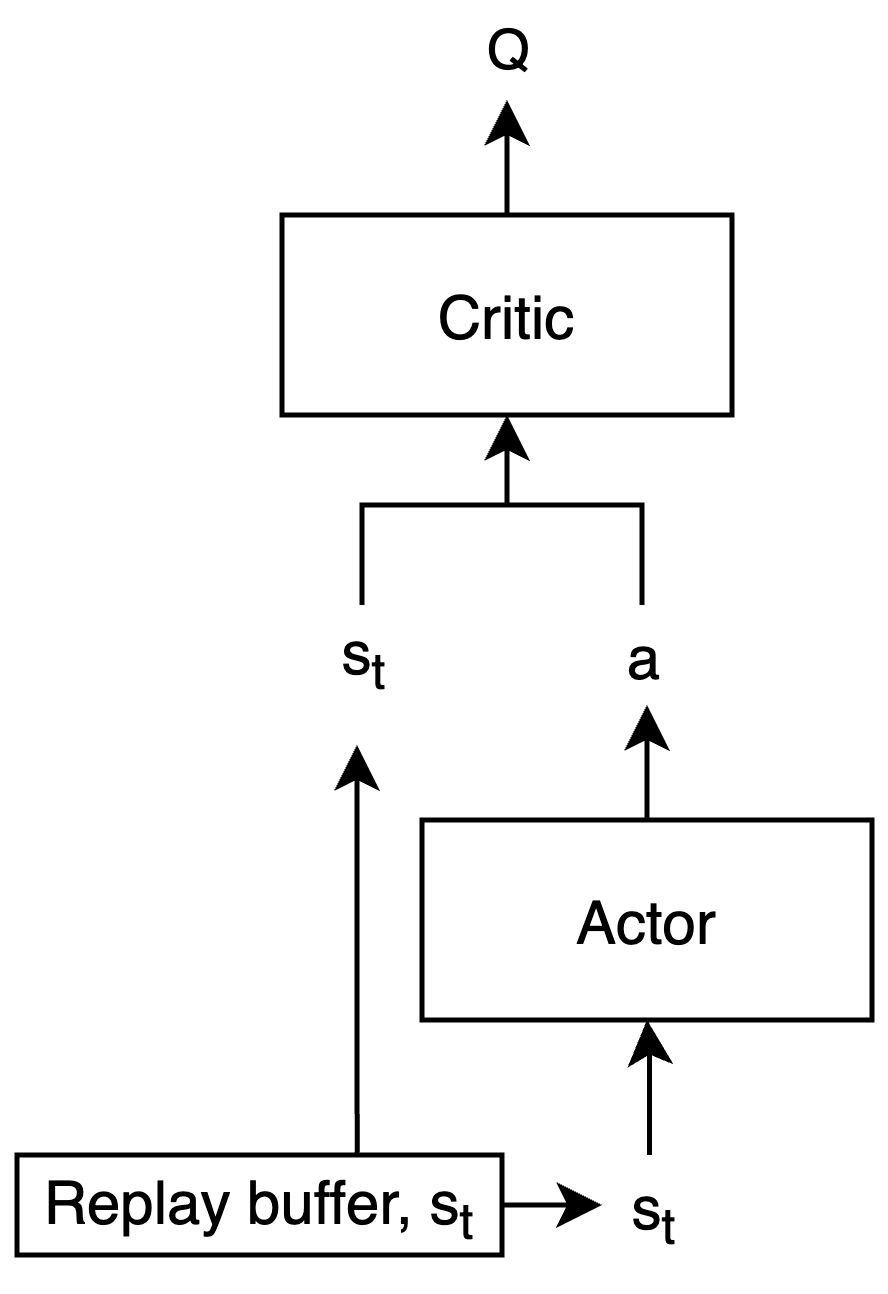
\includegraphics[width=\textwidth]{figures/3_/3_4_training_actor.png}
        \caption{Training the actor network}
        \label{fig:3_4_actor}
    \end{subfigure}
    \hfill
    \begin{subfigure}[b]{0.6\textwidth}
        \centering
        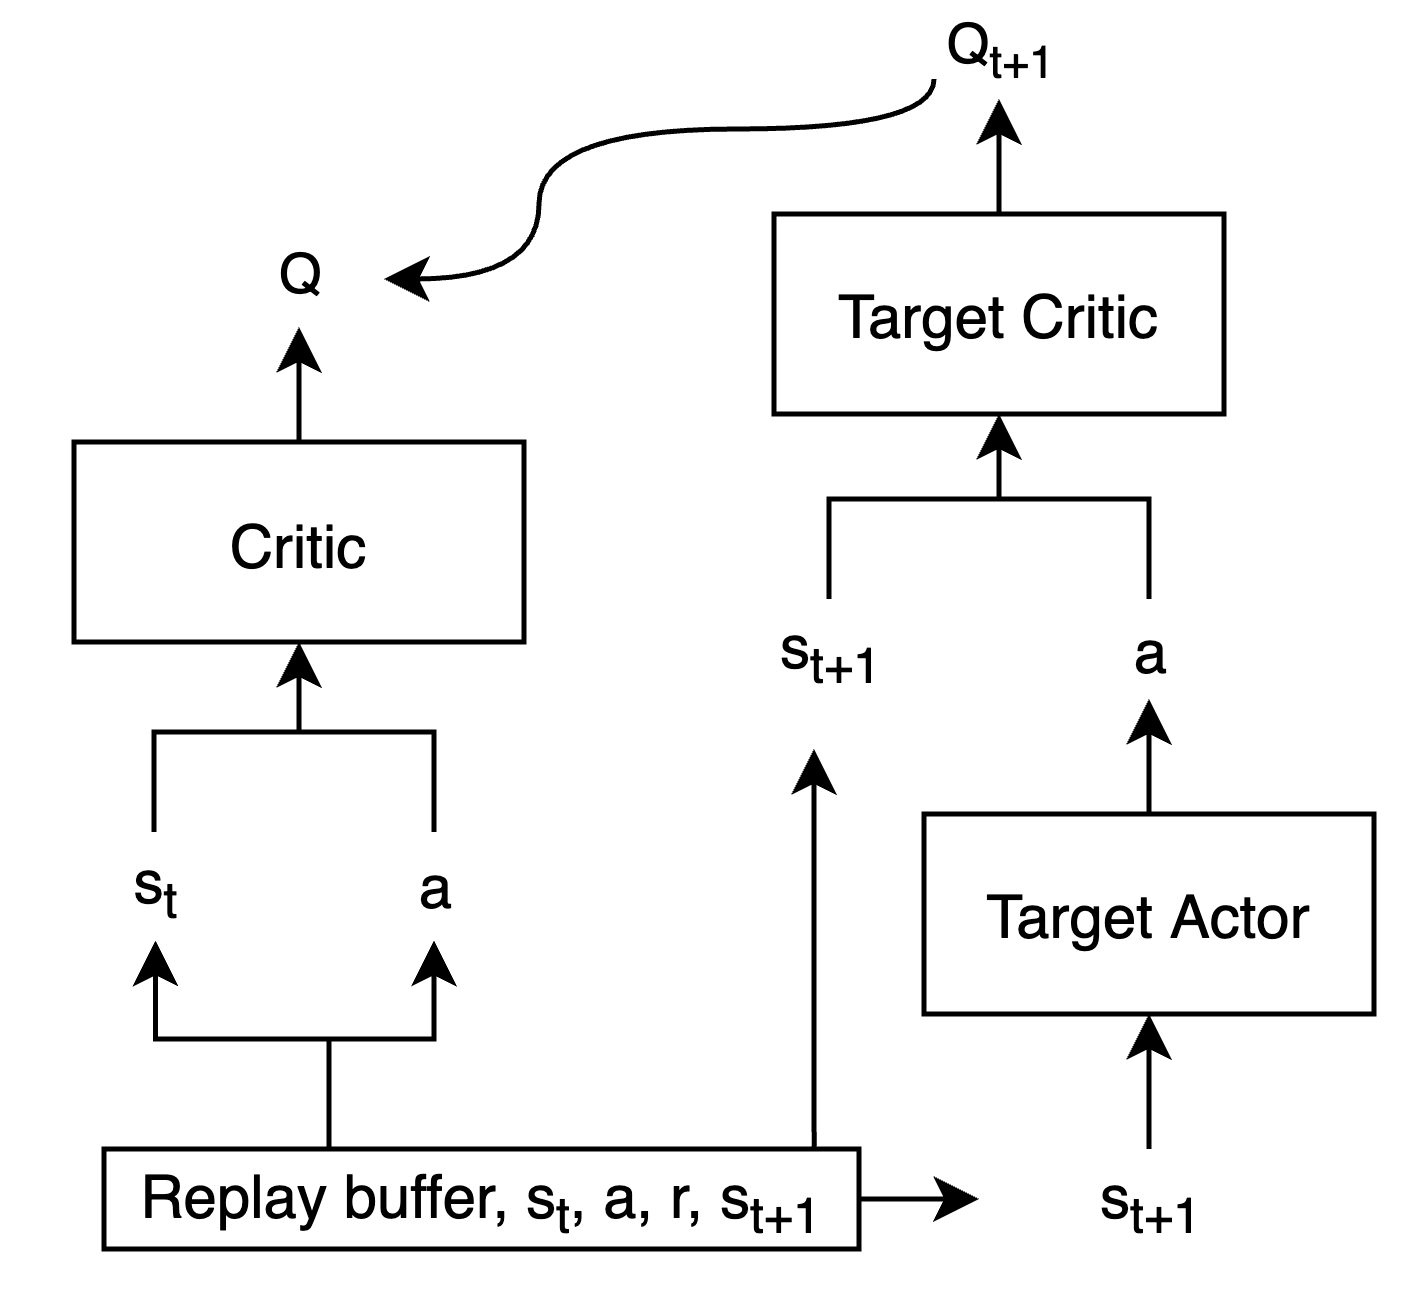
\includegraphics[width=\textwidth]{figures/3_/3_4_training_critic.png}
        \caption{Training the critic network}
        \label{fig:3_4_critic}
    \end{subfigure}
    \hfill
    \caption{An overview of how the actor and critic networks are updated in DDPG.}
    \label{fig:3_4_training}
\end{figure}
With a bit of understanding of the theory behind DDPG, it is insightful to have a more conceptual view over how DDPG is structured. From Figure \ref{fig:3_4_training}, we see that the actor network is updated as \eqref{3_4_actorGrad}, where the actor objective function $J(\btQ)$, which is $Q\,(S_t,\, \mu(S_t|\btmu)\,|\, \btQ)$, is backpropagated through the critic network and to the weights of the actor network. Similarly, we see that to obtain the prediction and the target of the loss in \eqref{3_4_NewcriticLoss}, we  sample the experience from the replay buffer, get our prediction term though our critic network, and get our target term through the target networks. Hence, we can calculate the MSE loss and backpropagate it to the critic network weights. Formally, backpropagation here simply refers to the method of calculating the gradient of the objective function or loss, with respect to the individual parameter weights of the network. Though informally, ``backpropagate it'' means to first find the gradient of the loss, w.r.t. the parameter weights, and then update the weights through gradient descent using the respective gradients.

\subsection{Summary}

DQN \cite{DQN} was able to solve Atari-based games from directly taking pixels as low-level observations as the state space. It was able to do this by adapting Q-learning \cite{watkins1992QLearning} with a NN as a parametrisation for the action-value function $Q$, along with the other innovations mentioned above. The universal function approximating ability of NNs allowed it to, in some sense, ``capture the features of the high dimensional observation space'', which allowed it to find an appropriate value estimate for each state with much fewer parameters than would otherwise be needed. So, by taking an image as input, the Q-network would have as output the value estimates for each possible action $a\in\mathcal{A}$ \cite{DQN}. The downside of this appears for problems that have high dimensional action spaces, as the size of output layer scales linearly with the number of actions.

DDPG follows the same idea as DQNs, but can in addition solve reinforcement learning problems with continuous (high-dimensional) observation and action spaces. 
This was achieved by using an actor-critic structure along with a NN parametrisation for the deterministic policy $\mu(s)$ and the action-value function $Q(s,a)$, where the additional actor gives DDPG the ability to learn how to output actions $a$, in the continuous action space, $\mathcal{A}$. Likewise, the critic $\Qt$, is able to take in this action $a$ along with an observation $s$, where both belong to continuous spaces, to output an appropriate action-value estimate. Then, to complete the cycle of the actor-critic structure, this action-value estimate can be used to train the actor network, as the gradient of the deterministic policy is simply the expected gradient of the action value function as shown in \eqref{3_4_actorGrad}. By being able to optimise this actor network to maximise its objective function, DDPG has thus the potential to obtain a policy capable of finding optimal actions in every state. 

Lastly, since DDPG is a model-free algorithm, it has the ability to perform well across learning tasks as it does not require any domain knowledge or transition dynamics, which follows from using \textit{Q}-learning to update the critic, as explained in Section \ref{sec:2_6_modelFreeContinuous}. This was also complemented by the fact that the DDPG uses \textit{batch normalisation}, so to generalise inputs into the actor and critic.
So with these characteristics, DDPG seems like a natural choice to use for the guidance task of this project.


\section{Proximal Policy Optimisation}
\label{sec:PPO}

In light of the advancements within reinforcement learning for robotics, a new family of methods was developed to curb the problem of instability and divergence when training agents using NNs. These are called \textit{trust-region} based policy optimisation methods, stemming from TRPO \cite{TRPO}.
PPO \cite{PPO} is heavily inspired by this, where the overarching idea is that in order to maintain stability in training, the new, updated policy should be within a specific \textit{trust-region} of the old policy, hence the name proximal policy.
As for its other characteristics, PPO is a also a model-free, on-policy and actor-critic method. In addition, it parametrises a stochastic policy $\pi(a\,|\,s)$ (unlike DDPG) and uses a uniquely defined objective function to optimise this.

\subsection{Advantage and some notation}
Earlier, we defined the policy gradient in \eqref{3_3_actorGrad}. This can be implemented in practice as:
\begin{equation}
    \widehat{\nbt J_t(\bt)} = \hatE \left[ 
    \frac{\nbt \pibt}{\pibt} \: \hatA (s, a) 
    \right] \label{3_5_actorGrad}
\end{equation}
where $\hatE$ represents the empirical average over a finite batch of samples of actions $a$ and states $s$. Also, we introduce a colloquial term $\hat{A}$, called the \textit{advantage} function $A : \mathcal{S} \times \mathcal{A} \rightarrow \mathbb{R}$, that represents how well an action did compared to some \textit{baseline} estimate:
\begin{equation}
    \hat{A}\,(s ,a) = \underbrace{Q\, (\,s,\, a\,)}_{\text{discounted return}} - \quad \underbrace{V_{\bt}\,(\,s\,)}_{\text{estimate}} \label{3_5_advantage}
\end{equation}
The baseline in this case is the parametrised value function $V_{\bt}$. Note that the first term shows the rewards that was actually received, while the second is an estimate of what we expected to receive in that state -- the critic. Hence, the advantage gives a picture of whether the agent performed better or worse than expected. 

We also introduce a slightly different notation here, where the subscript denotes the parameters to which the functions are parametrised with. Strictly speaking, the value functions should be taking in the random variables $S_t$ and $A_t$, but we assume the shorthand notation of $V_{\bt} (s) = V_{\bt} (S_t \,|\, S_t = s)$ for simplicity. This is also meant to prevent confusion with the advantage term $\hat{A}\,(s,a)$.

\subsection{PPO-Clip}
\label{subsec:PPO-clip}

PPO ensures that the new policy is close to the old one by using one of two tricks: clipping or an adaptive Kullback-Leibler (KL) divergence penalty term. Primarily, the one that is used is the \textit{clipped surrogate objective} version of PPO, which is also used in this project. In this version, the authors prevent large charges to the policy parametrisation by basically flattening the policy objective function to a certain maximum value. To visualise this, we can look at the novel objective function used.

PPO takes the surrogate objective function used by TRPO (whose gradient is equivalent to \eqref{3_5_actorGrad}):
\begin{equation}
    J_t(\bt) = \hatE \left[ 
    \frac{\pibt}{\pibtold} \: \hatA (s, a) 
    \right]
    = \hatE \left[ 
    r_t(\bt) \: \hatA (s, a) 
    \right]
\end{equation}
and clips it by a maximum value bounded by a hyperparameter $\epsilon$ to obtain the \textit{actor objective function}:
\begin{equation}
    J_t^{CLIP}(\bt) = \hatE \left[ \min\,(
    r_t(\bt) \: \hatA (s, a), \, \text{clip}\, ( r_t(\bt), 1-\epsilon, 1+\epsilon) \, \hatA(s,a)
    \right]
    \label{3_5_clippedObjective}
\end{equation}
This clipping aims to remove the incentive from deviating more than $\epsilon$ away from the old policy \cite{PPO} and can be visualised in Figure \ref{fig:3_5_clippedLoss}. Also, the ratio $r_t(\bt) = \frac{\pibt}{\pibtold}$ can be understood as the change in probability of selecting actions compared to the old policy, $\pibtold$, such that $r_t(\bt_{\text{old}}) = 1$.
\begin{figure}[htb]
    \centering
    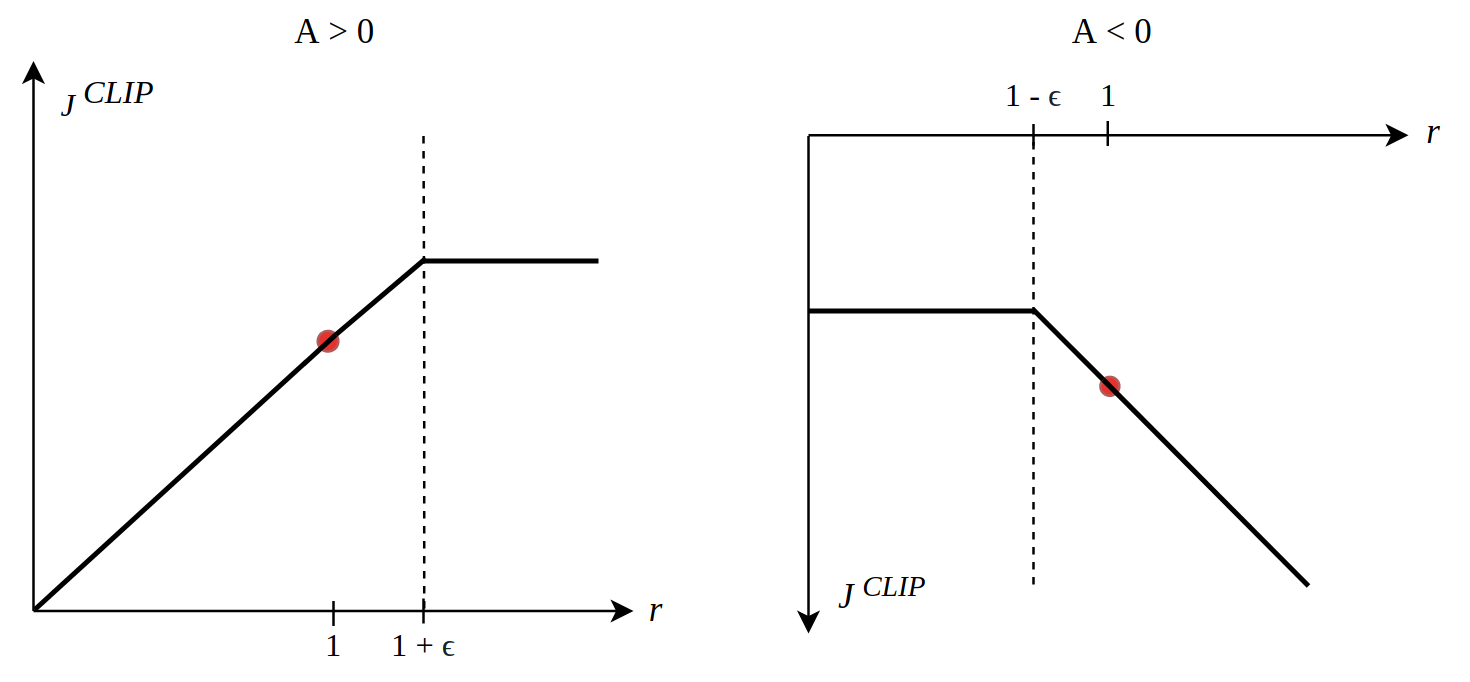
\includegraphics[width=0.8\textwidth]{figures/3_/3_5_clippedLoss.png}
    \caption{Visualising the clipped surrogate objective function for positive and negative advantages $A$. The figure is recreated from the original paper \cite{PPO}.}
    \label{fig:3_5_clippedLoss}
\end{figure}

The way to understand the clipped surrogate objective is to first remember that we are performing gradient ascent in the objective function, w.r.t. the policy parameters $\bt$. This means that we essentially choose the direction in which $r_t(\bt)$ should move in \eqref{3_5_clippedObjective} and Figure \ref{fig:3_5_clippedLoss}. When the agent performs better than expected, i.e. the advantage is positive, we wish to increase the probability of doing those actions again, which is equivalent to increasing $r_t(\bt)$. So, we adjust the parameters $\bt$ such that probability ratio $r_t(\bt)$ moves to the right. However, since we are taking the minimum and the objective is clipped at $1+\epsilon$, there is no added benefit of increasing $r_t(\bt)$ beyond this clipped point. Similarly, when the agent performs worse than expected, i.e. the advantage is negative, we wish to lower the probability of those actions happening again, which is equivalent to reducing the probability ratio $r_t(\bt)$. Again, since we clip the value at $1-\epsilon$ and the objective function is taking the minimum, there is no benefit of decreasing $r_t(\bt)$ beyond the clipped point. Therefore, by aiming to maximise the performance objective in \eqref{3_5_clippedObjective} by gradient ascent, the authors manage to prevent the new policy from deviating too far from the old one, as seen by $r_t(\bt)$ being discouraged to move beyond $[1-\epsilon, 1+\epsilon]$. 


\subsection{Actor-Critic Structure}
\label{subsec:3_ppo_actorCritic}
With the key idea from PPO presented, we can delve into the actor-critic structure of PPO. As shown above, the policy gradient is based on the advantage term $\hatA$. As a result, PPO uses a parametrisation of the value function $V(s)$ as a critic, so to produce an estimate for the advantage $\hatA$ in \eqref{3_5_advantage}.
Similarly to before \eqref{3_3_VE}, the parametrised value function can be optimised by minimising the mean-squared-error $\overline{VE}$:
\begin{equation}
    J_t^{VF}(\bt) = \E_t \Big[(V_{\bt_t}(s) - V_t^{\text{targ}})^2\Big] \label{3_5_criticLoss}
\end{equation}
where the target value function $V_t^{\text{targ}}$ that was implemented in the code of \cite{PPO} is defined as:
\begin{equation}
    V_t^{\text{targ}} = R_t + \gamma V_{\bt_t}(s')
\end{equation}
Lastly, there is an entropy term $S[\pi_{\bt}](s)$ that is also added to the objective function, which serves as an exploration term. 

So combined, the overall objective function for PPO with the actor objective function in \eqref{3_5_clippedObjective}, critic loss in \eqref{3_5_criticLoss} and entropy term, is:
\begin{equation}
    J_t^{CLIP+VF+S}(\bt) = \hatE \Big[
    J_t^{CLIP}(\bt) + c_1 J_t^{VF}(\bt) + c_2 S[\pi_{\bt}](s)
    \Big],   \label{3_5_objectiveFull}
\end{equation}
where $c_1$ and $c_2$ are coefficients. PPO also assumes that some automatic differentiation software is used, such that the software is able to keep track of how each objective function is computed in order to backpropagate the gradients appropriately. This also allows PPO to simply combine the objective functions like above.

Note that in the PPO implementation, the parameters $\bt$ characterise the whole actor-critic model, though ``under the hood'' they are indeed two different NNs that receive their own gradients. However, they have done this generalisation in the case where parameter-sharing is desired, where the ``bottom'' hidden layers are the same and the network heads are different. Moreover, since the actor is parametrising a stochastic policy, the head of the actor network outputs the parameters of the policy distribution, which for continuous cases is a Gaussian distribution.

Furthermore, one of the things to keep in mind is that PPO is also an on-policy algorithm. This means that when the agent is sampling experiences, these samples are gathered under its current policy $\pibt$. Hence, in its actor-critic implementation, a sample \textit{trajectory} of $T$ timesteps is first collected under a policy $\pibt$, before updates are made to the actor and critic parameters $\bt$. This means after $T$ timesteps, we have also received the rewards for each timestep and can compute the advantage estimates $\hatA$ for every timestep $t = 1, 2, ..., T$.
Then, when we are optimising the performance objective, we have the opportunity to define how many epochs $K$ was in that trajectory of size $T$, which means that we can specify how many gradient updates to do using the same batch of experiences. After the updates are completed, we discard this trajectory of experiences and begin sampling a new one, to ensure that the new experiences occur under the new policy $\pi_{\bt}$. 
\begin{figure}[ht]
    \centering
    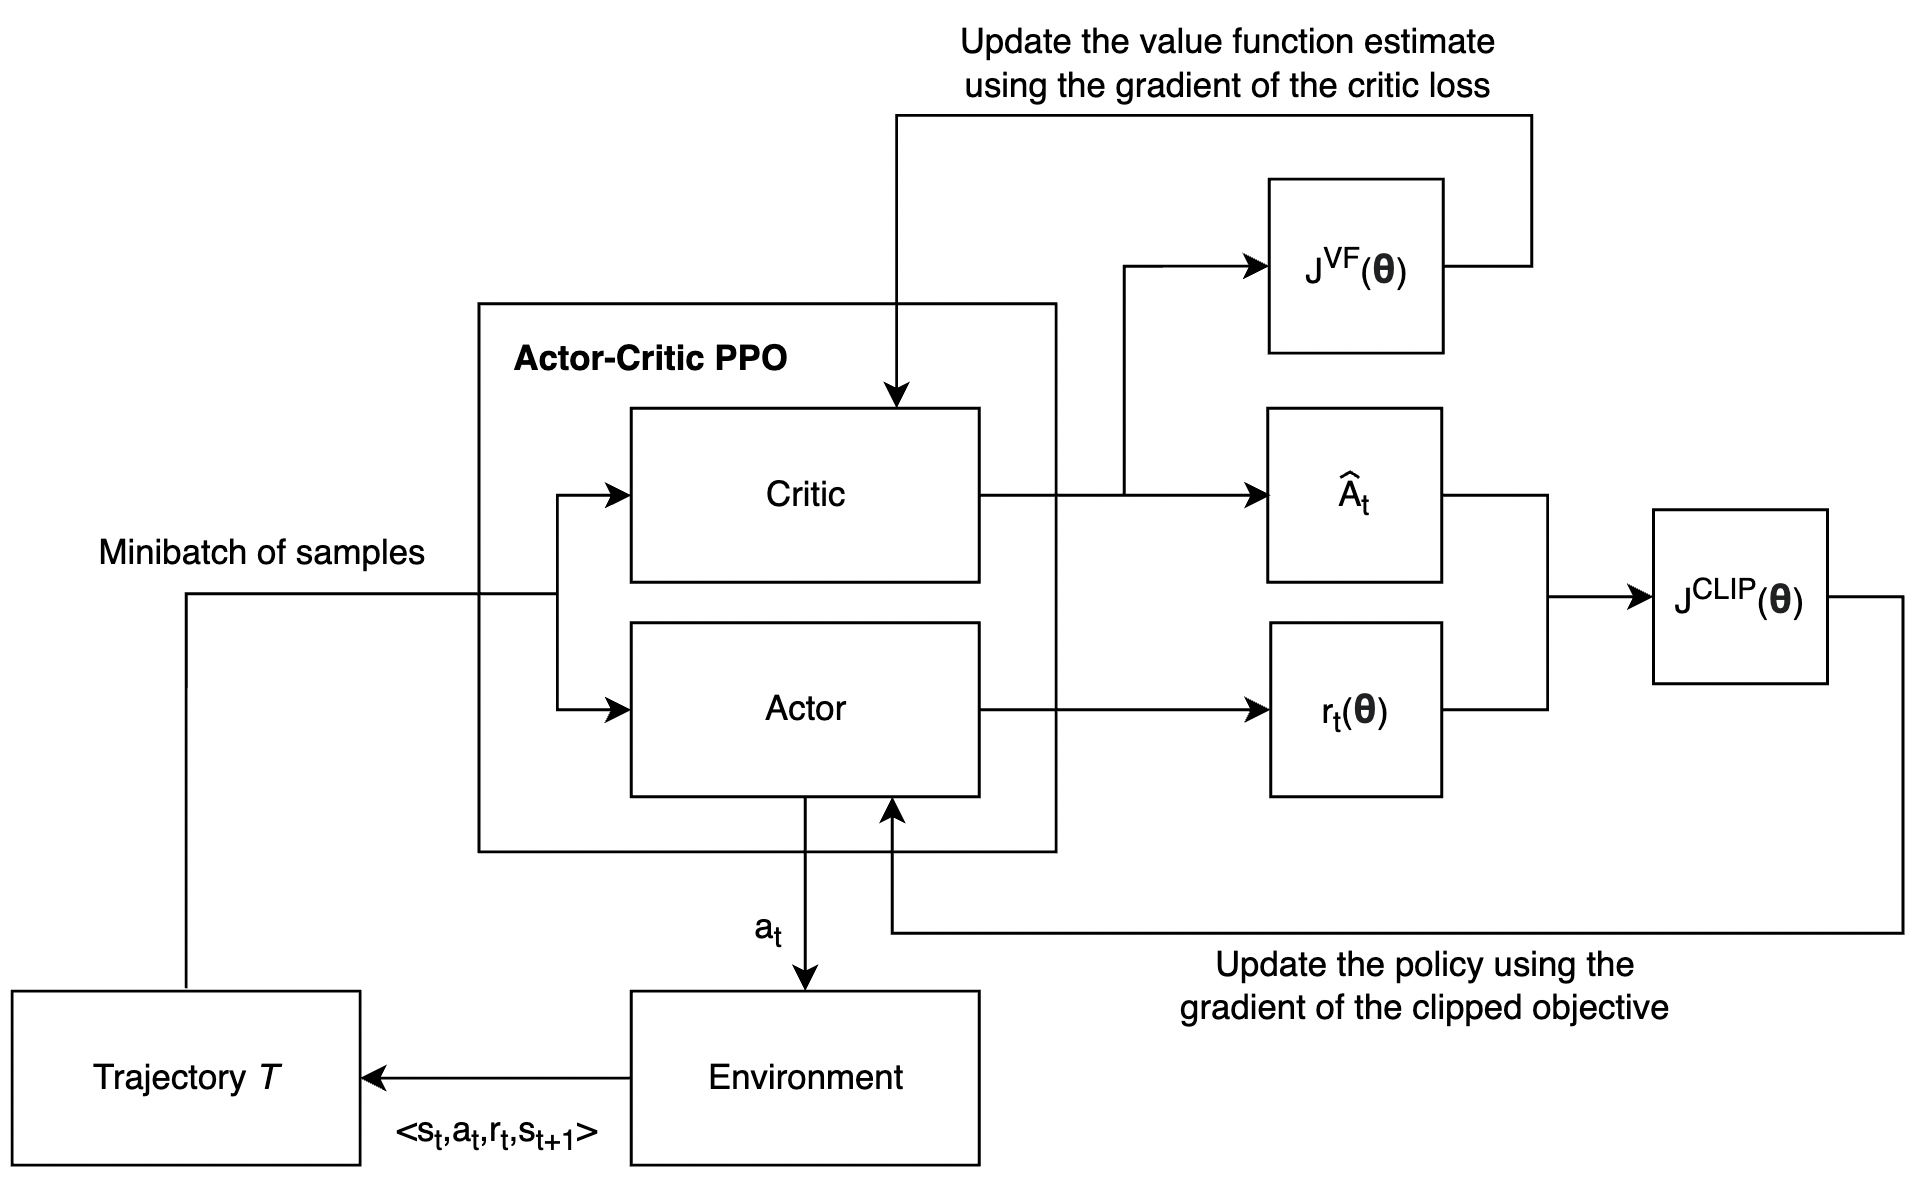
\includegraphics[width=0.95\textwidth]{figures/3_/3_5_ppoOverview.png}
    \caption{An overview of how the actor and critic networks are updated in PPO. Once the loss terms are calculated, the gradients $\nabla J_t^{CLIP}(\bt)$ and  $\nabla J_t^{VF}(\bt)$ are used to update the actor and critic respectively.}
    \label{fig:3_5_ppoTraining}
\end{figure}
Conceptually, we can view the whole update process in Figure \ref{fig:3_5_ppoTraining}. Here, we first see that a trajectory is sampled based on the current policy given by the actor, before the loss terms are calculated. Finally, the gradient of the objective function w.r.t. to the actor and critic weights is used to update the actor and critic networks.

\subsection{Summary}
PPO is able to solve a vast variety of continuous reinforcement learning problems by being a model-free, actor-critic method and using NNs as function approximators. It is also an on-policy method, meaning the sampled trajectory of experiences are collected under its current policy $\pibt$. The algorithm is able to achieve state-of-the-art performances through its adaptation of the trust-region based method, TRPO, where the idea is to take the largest possible step in the right direction, but while ensuring that the new policies, after an update, stay close (or are \textit{proximal}) to the old one. This in turn, as stated in TRPO \cite{TRPO}, should guarantee a monotonic improvement of the policy.

In terms of implementation, it is relatively simple compared to its counterpart, TRPO. It uses a clipped surrogate objective to define its proximal policy aim, rather than a hard constraint that requires second-order methods to optimise. Also, as it assumes we are using an automatic differentiation software, we can combine the objective functions for both the policy and the value function parametrisations, where the software is able to keep track of how to compute the gradients (perform backpropagation) for the respective parameters.

Also, since it is on-policy like TRPO, it retains its supposedly high data-efficiency and reliable performance. This is particularly significant for problems with high-dimensional state and action spaces, since the agent can focus on exploring actions along its current policy instead of obtaining needless gradients from actions in states that are very uncommon. This is also a reason why it is more data-efficient, as it is able to converge to an optimal behaviour faster.

However, since PPO is on-policy, the overall degree of exploration is based largely on its stochastic policy $\pibt$, with the exception of the entropy term. However, as discussed in the end of section \ref{sec:3_3_actor-critic}, this means that the agent may suffer from a lack of exploration if its policy does not incorporate some degree of randomness. Yet, by the nature of optimisation, PPO will progressively increase probabilities of doing ``good'' actions and decrease probabilities of doing ``bad'' ones, based on its estimate of advantage and value function. This means that over time, the agent will exploit the environment more, irrespective of how accurate its estimate of the policy and value function is, and could become trapped in a local optima.

\chapter{Method}
\label{chap:method}

\section{Problem formulation}
\begin{comment}

Problem formulation, - state, action, what is our goal.
then with dynamics of quadrotor. 
After have PD controller under this.
Basic RL methods for this project
what use RL for in this project
Implementation
Experimental setup
\end{comment}

The task of this project is to evaluate the performance of DDPG and PPO as guidance systems in the context of quadrotor waypoint navigation.
Guidance in this case can be defined as “the process for guiding the path of an object towards a given point, which in general may be moving” \cite{shneydor1998Guidance} or ``a basic methodology concerned with the transient motion behavior associated with the achievement of motion control objectives'' \cite{Fossen2021}. As such, we can define the reinforcement learning objective as \textit{deciding the motion of a quadrotor through desired acceleration, such that it is able to reach a desired end position in 3-dimensional space.}

In a reinforcement learning context, the learning task thus becomes to discover an optimal policy that chooses an  action $A_t \in \mathcal{A}$ when in a state $S_t \in \mathcal{S}$, so that our state $S_t$ converges to some goal state as $t \rightarrow T$, where $T$ represents the end timestep of an episode. Our state and action is defined as:
\begin{equation}
    S_t = 
    \begin{bmatrix}
    \p_t^\top & \v_t^\top% x,y,z, u,v,w 
    \end{bmatrix} ^ \top, \qquad
    A_t = 
    \begin{bmatrix}
    \a_t
    \end{bmatrix}
    \label{4_1_stateActionsSpace}
\end{equation}
where $\p$, $\v \in \mathbb{R}^3$ denote the generalised position and velocity of the quadrotor with respect to the goal frame, $\{\text{goal}\}$, while and $\a$ denotes the acceleration of the quadrotor with respect to the body-fixed frame, $\{\text{b}\}$:
\begin{equation}
    \p_t^\text{goal} = \begin{bmatrix}
    x_t & y_t & z_t
    \end{bmatrix}^\top, \quad
    \v_t^\text{goal} = \begin{bmatrix}
    u_t & v_t & w_t
    \end{bmatrix}^\top, \quad
    \a_t^\text{b} = \begin{bmatrix}
    \Dot{u_t} & \Dot{v_t} & \Dot{w_t}
    \end{bmatrix}^\top
\end{equation}
Furthermore, the goal frame is stationary and represents an approximate inertial frame. The desired goal state is then chosen to be the origin of the goal frame, represented by the point $\p^\text{goal}_g = [0,0,0]^\top$.
From this, we see that the problem of waypoint navigation essentially becomes a task of setpoint regulation, where we wish to regulate our quadrotor position, $\p_t^\text{goal}$ to \textbf{0}.

As the reinforcement learning agents are responsible solely for the guidance of the quadrotor, we assume that there exists an underlying basic control system that is able to allocate the control inputs so as to produce the desired acceleration.
So, in the following section we will discuss how these accelerations are interpreted in the control system, before moving on to how we are able to implement the algorithms in practice and how exactly we will evaluate the DDPG and PPO algorithms.


\section{Dynamics of a Quadrotor}
\label{sec:4_dynamics}
In this section, we aim to cover the dynamics of the quadrotor through its rigid-body equations of motions, before moving on to the relationship between desired accelerations and generated forces in the feedback control system. Finally, we conclude with a description of the control allocation, showing how output torques from the control system is distributed to the individual rotors.

\subsection{Rigid-body Dynamics}
\label{sec:4_2_dynamics}
As the overall task of the reinforcement learning agent is to decide the motion of the quadrotor through acceleration, a natural first step is to understand how motion is achieved through the quadrotor rigid-body equations of motion.

To simplify notation, we define a right-hand inertial frame \{\textit{n}\} (e.g. the goal frame), and use \{\textit{b}\} to represent the the body-fixed frame as in the previous section. From \cite{MultirotorAerialVehicles} and using notation from \cite{Fossen2021}, we can then express the dynamics of the quadrotor as:
\begin{align}
    \Dot{\p}^n_{nb} &= \v^n_{nb} \\
    m \Dot{\v}^n_{nb} &= m\boldsymbol{g}^n + \boldsymbol{R} (\boldsymbol{\Theta}_{nb}) \, \boldsymbol{f}^b \label{4_1_transKinetics} \\ 
    \Dot{\boldsymbol{\Theta}}_{nb} &= \boldsymbol{\Theta}_{nb} \boldsymbol{\omega}^b_{nb_\times} \\
    \boldsymbol{I}^b_b\Dot{\boldsymbol{\omega}}^b &= - \boldsymbol{\omega}^b_{nb} \times \boldsymbol{I}^b_b\boldsymbol{\omega}^b_{nb} + \boldsymbol{\tau}^b  \label{4_1_rotKinetics}
\end{align}
\begin{table}[h]
    \centering
    \begin{tabular}{ll}
        $\boldsymbol{p^n_{nb}} \in \R^3$        & position of the quadrotor body-frame $\{b\}$ w.r.t. to $\{n\}$, expressed in $\{n\}$ \vspace{0.8mm} \\
        
        $\boldsymbol{v^n_{nb}} \in \R^3$        & velocity of the quadrotor body-frame $\{b\}$ w.r.t. $\{n\}$ expressed in $\{n\}$ \vspace{0.8mm} \\
        
        $m \in \R$                              & mass of the quadrotor \vspace{0.8mm} \\
        
        $\boldsymbol{g}^n \in \R^3$             &  gravitational acceleration $[0, 0, -g]^\top$, where \textit{g} = 9.81  ms$^{-2}$\vspace{0.8mm} \\
        
        $\boldsymbol{R} \in SO(3)$              & Euler angle rotation matrix from \{\textit{b}\} to \{\textit{n}\}, with argument $\boldsymbol{\Theta}_{nb}$ \vspace{0.8mm} \\
        
        $\boldsymbol{\Theta}_{nb} \in \R^3$     & orientation of the body-fixed frame \{\textit{b}\} w.r.t. \{\textit{n}\}, expressed with roll, \\ &pitch, yaw angles $[\phi, \theta,\psi]$ \vspace{0.8mm} \\
        
        $\boldsymbol{\omega}^b_{nb} \in \R^3$   & angular velocity of the quadrotor  body-frame $\{b\}$ w.r.t. $\{n\}$, expressed in $\{n\}$ \vspace{0.8mm} \\ 
        
        $\boldsymbol{\omega}^b_{nb_\times} \in \R^{3\times3}$ & skew-symmetric representation of $\boldsymbol{\omega}_{nb}$ \vspace{0.8mm} \\
        
        $\boldsymbol{I}^b_b \in \mathbb{R}^{3\times3}$ & inertia dyadic of the quadrotor body-fixed frame \{\textit{b}\}, expressed in \{\textit{b}\} \vspace{0.8mm} \\
        
        $\boldsymbol{f}^b \in \R^3$             & external forces applied to the quadrotor body frame $\{b\}$, expressed in \{\textit{b}\} \vspace{0.8mm} \\
        
        $\boldsymbol{\tau}^b \in \R^3$          & external moments applied to the quadrotor body frame $\{b\}$, expressed in \{\textit{b}\}
    \end{tabular}
    \caption{Notation used in the quadrotor rigid-body equations of motion.}
    \label{table:parameters}
\end{table}

Note that the subscripts $\{n\}$ and \{\textit{b}\} for $\Dot{\p}^n_{nb}$ and $\Dot{\v}^n_{nb}$ simply emphasise that the position and velocities are the movements of the body frame \{\textit{b}\} with respect to the inertia frame $\{n\}$, expressed in $\{n\}$, following from \cite{Fossen2021}. This is in contrast to Equation \eqref{4_1_stateActionsSpace}, where we denote $\Dot{\p}^n_t$ and $\Dot{\v}^n_t$ to show that these positions and velocities change with time.
The coordinate frames, along with the alignment of the body-fixed frame on the quadrotor can be seen in Figure \ref{fig:4_1_quadrotorBody}.
\begin{figure}[hbt]
    \centering
    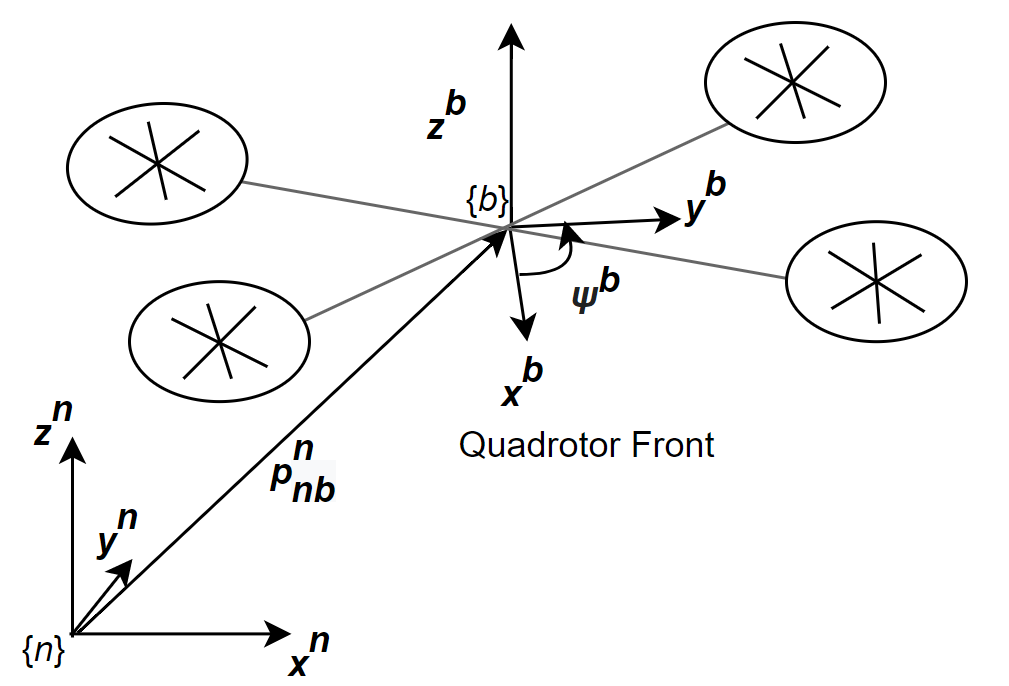
\includegraphics[width=0.7\textwidth]{figures/4_/4_2_quadrotorBody.png}
    \caption{An illustration of the relevant quadrotor coordinate frames. We have an inertial frame \{\textit{n}\} and a body frame \{\textit{b}\}.}
    \label{fig:4_1_quadrotorBody}
\end{figure}

Looking at equations of motion, we see a system with six degrees of freedom: three translational and three rotational. 
However, for a quadrotor, this means that we have an underactuated system. To illustrate this, the rotors have an arm that extends from the body-frame origin to the centers of each rotor. Since, these arms span the $\x^b\y^b$-plane and all of them produce a perpendicular thrust upwards along $\z^b$, we can mentally visualise that the quadrotor is able to produce torques to directly influence our roll $\phi$ and pitch $\theta$ angles, as well as a total force along $\z^b$. However, if our quadrotor body-frame \{$b$\} is aligned with the inertia frame \{$n$\}, all rotors produce a thrust parallel to $\z^n$ such that we cannot directly produce a vector thrust that spans the $\x^n\y^n$-plane, and hence our system is underactuated in these degrees of freedom. 

\begin{comment}
Formally, this is shown as \cite{Fossen2021}:
\begin{equation}
    \begin{bmatrix}
    \boldsymbol{f}^b \\
    \boldsymbol{\tau}^b
    \end{bmatrix}
    = \begin{bmatrix}
    \boldsymbol{f}^b \\
    \boldsymbol{r}^b_{tb} \times \boldsymbol{f}^b
    \end{bmatrix}
    = \begin{bmatrix}
    F_x \\
    F_y \\
    F_z \\
    l_y F_z - l_z F_y \\
    l_z F_z - l_x F_z \\
    l_x F_z - l_y F_x
    \end{bmatrix}
    \label{4_1_forceToThrust}
\end{equation}
where $\boldsymbol{r}^b_{tb} = [l_x, l_y, l_z]$ is the vector of lever arms from $\{b\}$ to the rotor centers, and $\boldsymbol{f}^b = [F_x, F_y, F_z]$ being the thrust vector decomposed in $\{b\}$ as before.
From this, we note that all degrees of freedom apart from 1 and 2 are non-zero, as $F_x$ and $F_y$ are zero. 
--In the hovering case, F_z is centered around the origin so all arms are 0. This means that only DOF 3 is non-zero so example could be confusing. 16/12
\end{comment}

So, to get be able to generate surge and sway velocities $u$ and $v$, the quadrotor has to exploit the system dynamics. Simply put, in order to accelerate along the $\x^n$ and $\y^n$ axes, the quadrotor can rotate its body-frame such that the overall thrust (along $\z^b$) points forward or sideways when decomposed $\{n\}$. This is shown in Equation \eqref{4_1_transKinetics}, where we see that accelerations $\Dot{\v}^n_{nb}$ in the inertial frame are proportional to the rotated force vector, $\boldsymbol{R} (\boldsymbol{\Theta}_{nb})\, \boldsymbol{f}^b$. For the sake of completeness, we can write this explicitly:
\begin{equation}
    \boldsymbol{R} (\boldsymbol{\Theta}_{nb}) = \begin{bmatrix}
    c\psi c\theta & -s\psi c\phi + c\psi s\theta s\phi & s\psi s\phi + c\psi s\theta c\phi \\
    s\psi c\theta & c\psi c\phi + s\psi s\theta s\phi & -c\psi s\phi + s\psi s\theta c\phi \\
    -s\theta &  c\theta s\phi & c\theta c\phi 
    \end{bmatrix}
\end{equation}
where, $c$ and $s$ refer to shorthand notations for sin and cos. Thus, if we denote $\boldsymbol{f}^b$ as $[0,0,F_z]^\top$, we can express accelerations $\dot u$ along $\x^n$ (roll $\phi$, yaw $\psi$ small), and $\dot v$ along $\y^n$ (pitch $\theta$, yaw $\psi$ small) as:
\begin{align}
    \dot u &= \frac{F_z}{m} \sin{\theta} \label{4_2_udot} \\
    \dot v &= - \frac{F_z}{m} \sin{\phi} \label{4_2_vdot}
\end{align}
From this, it is clear to see that to accelerate forward along $\x^b$, we have to command a positive rotation in pitch $\theta$, while to accelerate left along $\y^b$, we have to command a negative rotation in roll $\phi$. 

\subsection{Control Allocation}
With the overall relationship between forces and rotor thrust established, we can include a brief note on how the rotor thrusts relate to angular velocities.
As already hinted, the total thrust $T_\Sigma$ of a quadrotor can be represented as the sum of individual thrusts from each rotor:
\begin{equation}
    T_\Sigma = \sum^N_{i=1} |T_i| = c_T \sum^N_{i=1} \Bar{\omega}_i^2 \label{4_2_totalThrust}
\end{equation}
where,
\begin{equation}
    T_i = c_T \Bar{\omega}_i^2 = C_T \rho A_{r_i} r_i^2 \Bar{\omega}_i^2
\end{equation}
Here, $\Bar{\omega}_i$ is the angular velocity of rotor $i$ and $c_T$ is a product of some constant parameters: $C_T$ being the thrust coefficient, $\rho$ the density of air, $A_{r_i}$ the rotor disk area and $r_i$ the radius of rotor $i$. So, as mentioned before, by the geometry of the quadrotor we can express the force vector $\boldsymbol{f}^b$, as the overall thrust upwards along $\z^b$:
\begin{equation}
    \boldsymbol{f^b} = T_\Sigma \cdot \z^b + \Delta
\end{equation}
where $\Delta$ represents unmodelled aerodynamic forces when the rotor is not stationary \cite{MultirotorAerialVehicles}. 

Next, we can define the reaction torque acting on the quadrotor body, i.e. the rotational force experienced around $\z^b$, as:
\begin{equation}
    Q_i = c_Q \Bar{\omega}_i^2
\end{equation}
where $c_Q$ is a product of some constants similar to $c_T$ \cite{MultirotorAerialVehicles}. Quadrotors are designed such that every other rotor spins the opposite direction such that the sum of reaction torques are 0. The first rotor, $i=0$ (following from $\x^b$ going around $\z^b$) spins in an anti-clockwise positive rotation around $\z^b$, while the next spins clockwise and so on.

Lastly, as we are interested in commanding $\dot u$ and $\dot v$ accelerations through roll and pitch angles, we will have to consider the how torques around $\x^b$ and $\y^b$ are related to the rotor angular velocities $\Bar{\omega}_i$. This moment is given by the standard equation of a thrust $T_i$ multiplied by a lever arm $d_i$. Since the body-frame axes $\x^b,\y^b$ do not align with the airframe rotor-arm, we take the projection of these arms onto the  $\x^b,\y^b$ axes, where the angles between the axes and rotor-arms are $\pm$45$\degree$.

Knowing this, we can combine with \eqref{4_2_totalThrust}, and define $\boldsymbol{\tau} = \boldsymbol{B} \boldsymbol{\Bar{\omega}}$ such as:
\begin{equation}
    \begin{bmatrix}
        T_\Sigma \\ \boldsymbol{\tau}^b
    \end{bmatrix}
    = \begin{bmatrix}
        T_\Sigma \\ \tau_1 \\ \tau_2 \\ \tau_3
    \end{bmatrix}
    = \underbrace{
        \begin{bmatrix} 
            c_T & c_T & c_T & c_T \\ 
            d\frac{\sqrt{2}}{2} & d\frac{\sqrt{2}}{2} & -d\frac{\sqrt{2}}{2} & -d\frac{\sqrt{2}}{2} \\ 
            -d\frac{\sqrt{2}}{2} & d\frac{\sqrt{2}}{2} & d\frac{\sqrt{2}}{2} & -d\frac{\sqrt{2}}{2} \\ 
            -c_Q & c_Q & -c_Q & c_Q 
        \end{bmatrix}
    }_{\boldsymbol{B}}
    \begin{bmatrix}
    \Bar{\omega}_1^2 \\
    \Bar{\omega}_2^2 \\
    \Bar{\omega}_3^2 \\
    \Bar{\omega}_4^2 \\
    \end{bmatrix}
    \label{4_2_controlAllocation}
\end{equation}
From this, we can find the angular velocities $\boldsymbol{\Bar{\omega}}$, for a desired set of torques and thrust $\boldsymbol{\tau}$, by taking the inverse of the control allocation matrix $\boldsymbol{B}$ and solving the inverse equation $\boldsymbol{\Bar{\omega}} = \boldsymbol{B}^{-1} \boldsymbol{\tau}$.  


\section{Role of Reinforcement Learning}

Now the quadrotor dynamics is understood, we can look into how reinforcement learning will be used specifically. As mentioned, our action space in \eqref{4_1_stateActionsSpace} is the acceleration vector $\a^b_t$ expressed in the body frame, $\{b\}$. Essentially, this is indirectly achieved by commanding a roll $\phi$ and pitch $\theta$ angle, as shown in \eqref{4_2_udot}, \eqref{4_2_vdot}. The relationship made between the desired acceleration and the roll and pitch angles is done in the basic control layer -- the PD controller -- which then uses the rotational kinetics in \eqref{4_1_rotKinetics} and the control allocation in \eqref{4_2_controlAllocation}, to produce the correct rotor angular velocities.

Conventionally, this means that our reinforcement learning agent represents an optimal control layer, or optimal controller, that serves as a guidance system that determines the optimal next-states in the waypoint navigation task. This makes sense as the reinforcement learning problem can be expressed as an optimisation problem, when considering large state-action spaces as mentioned in Section \ref{sec:2_6_modelFreeContinuous}. 
\begin{figure}[ht]
    \centering
    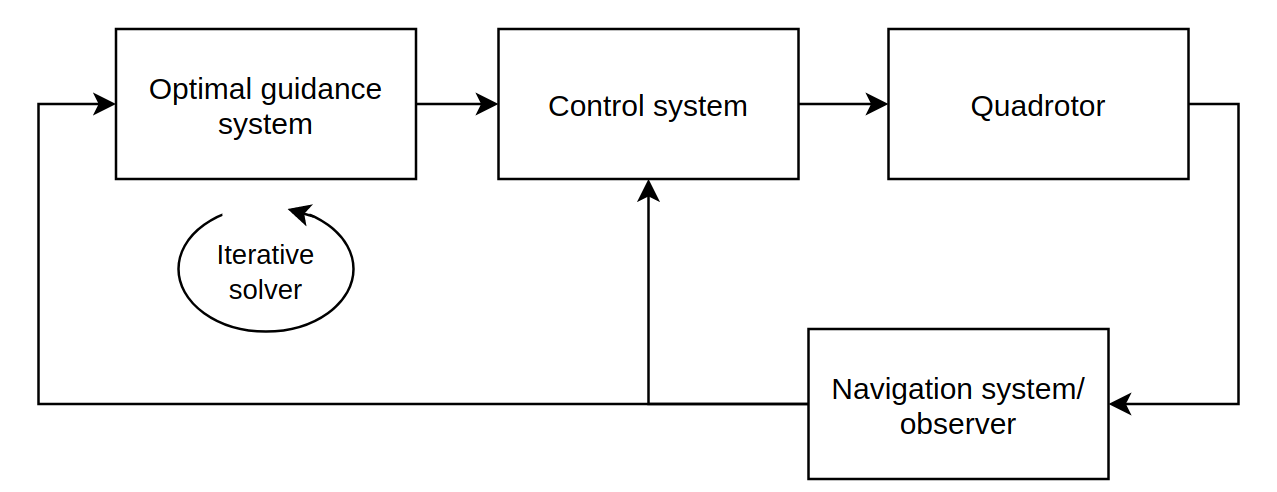
\includegraphics[width=0.8\textwidth]{figures/4_/4_1_Guidance.png}
    \caption{Traditional optimal trajectory generation using an iterative solver to an optimisation problem. Recreated from \cite{Fossen2021}.}
    \label{fig:4_3_Guidance}
\end{figure}
\begin{figure}[ht]
    \centering
    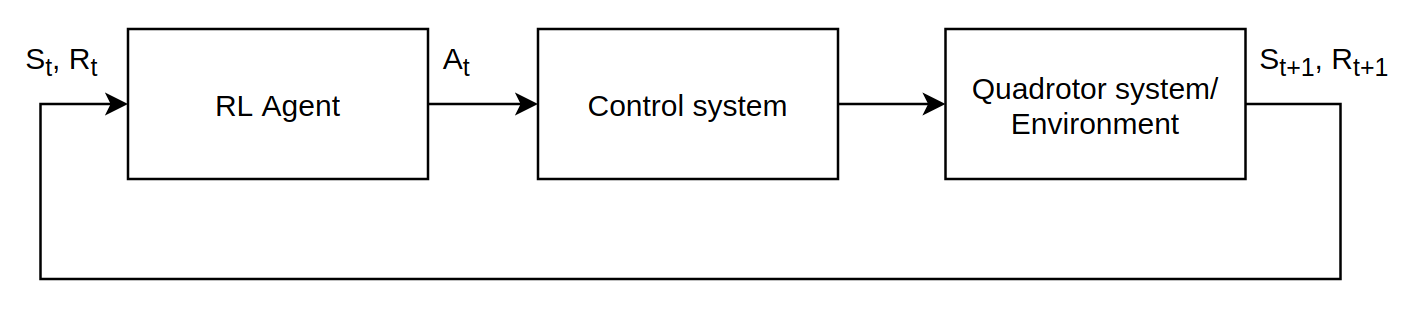
\includegraphics[width=0.9\textwidth]{figures/4_/4_1_RLGuidance.png}
    \caption{Using the reinforcement learning agents, DDPG and PPO, as optimal guidance systems that send accelerations (roll, pitch and height references) to the control system.}
    \label{fig:4_3_RLGuidance}
\end{figure}

Figure \ref{fig:4_3_Guidance} shows the classic setup of a guidance, navigation and control system, where the optimal trajectory is can be generated through a minimisation of a specific cost function, such as in quadratic programming (QP). Moving on, we see that the role of our DDPG and PPO algorithms will be to undertake the guidance system, such that our overall system transforms to Figure \ref{fig:4_3_RLGuidance}.

It is also not uncommon to use reinforcement learning agents to replace both guidance and control systems, such that the agents have to learn the mapping from their states $S_t$ to individual rotor thrusts $T_i$. This is for example done in \cite{ControlofQuadrotorRL} and \cite{song2021droneRacing}, where they have achieved excellent results. Otherwise, in \cite{PPOQuadrotor}, a step further was taken as states were mapped directly to rotor angular velocities. Nonetheless, we do not follow these approaches, but choose rather to utilise the underlying PD-controller. This makes our state and action spaces most alike \cite{RodriguezRamos2019ADR}, though ours is extended to three dimensional space.

The benefit of having a ``high'' abstraction output is that the learning task becomes more simplified as there are less physical relationships that needs to be learned. Instead, a PD controller can be used to leverage the underlying dynamics as we have good models for these. The downside however, is that through commanded accelerations we assume that the roll and pitch angles represent their desired values: $\phi = \phi_d$ and $\theta = \theta_d$. This entails that there must be a significant bandwidth separation between the reinforcement learning agent ``action frequency'' and the closed-loop control system bandwidth, so that this expectation is realistic. However, this is a possible limitation in the performance of the reinforcement learning agent as it cannot react as quickly to disturbances.

\section{Implementation}
In this section, we will look into how we can compare the DDPG and PPO algorithms from a practical perspective. To do this, we will look into how guidance and control of a quadrotor can be done through simulation, using a physics-based simulator called Gazebo \cite{Gazebo}.
Specifically, we will look into the different modules that are a part of the Gazebo framework, starting first with our quadrotor, then how this can be simulated, and finally how the algorithms are integrated into this system. Lastly, we will see how these modules are integrated into one complete system using the Robot Operating System (ROS).

The quadrotor used during this project is a model of the resilient micro-flyer (RMF), which is a collision-tolerant quadrotor well suited for navigation in a confined environment. The quadrotor can be visualised in Figure \ref{fig:4_1_rmf} below.
\begin{figure}[hbt]
    \centering
    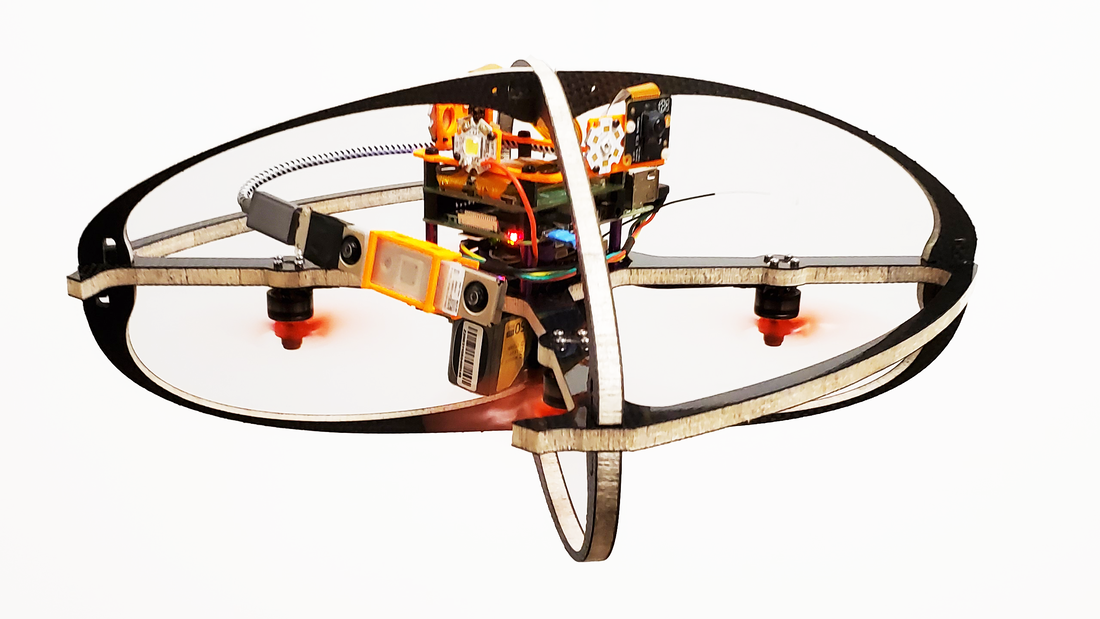
\includegraphics[width=0.5\textwidth]{figures/4_/rf-side-view-free-flight_orig.png}
    \caption{An image of an actual RMF, taken from \href{https://www.autonomousrobotslab.com/}{Autonomous Robots Lab}}
    \label{fig:4_1_rmf}
\end{figure}


\subsection{Gazebo}

The Gazebo \cite{Gazebo} physics-based simulation framework serves as a more realistic alternative compared to other simpler reinforcement learning environments, such as OpenAI Gym or Atari-based games. It allows its users to create models of their own robotic system, with custom sensors and actuators added, where it is then able to determine the dynamical response for this system given some external or control forces. This makes it an ideal choice for researchers looking to develop and test their algorithms, without requiring or risking a real robotic system.

To be able to simulate the RMF quadrotor seen in Figure \ref{fig:4_1_rmf}, we use a combination of a micro aerial vehicle (MAV) simulator, namely the \textit{RotorS} extension \cite{RotorS_Furrer2016}, together with some RMF Unified Robotic Description Format (URDF) files, to yield an RMF simulator.
The RotorS extension is a quadrotor simulator that the contains a variety of elements, such as an IMU, generic odometry sensor, visual-inertial sensor, autopilot, along with some quadrotor models \cite{RotorS_Furrer2016}.
The URDF files contains information about the RMF specific sensors, shape, weight, etc., describing all elements of the RMF.
Thus, by creating a workspace that includes these extensions, we then achieve a RMF simulator that is able to run fast and accurate simulations of the RMF quadrotor, risk-free.

But before we are able to command the quadrotor through RotorS, we need a way to do reinforcement learning with this system. If we recall from section \ref{chap:background_RL}, we essentially need an MDP environment for which the agent can perform actions in. As such, we used a wrapper for RotorS that served as both an environment and a method to communicate with the simulator. 
This wrapper allowed us to emulate a typical OpenAI gym environment, which then made it possible to use OpenAI's baseline implementations of DDPG and PPO \cite{baselines}.

So finally, we have a system where the agent, the DDPG or PPO algorithms, is able to interact with the RMF quadrotor environment through a RotorS wrapper, which further communicates the agent's decisions via messages to the simulator.
\begin{figure}[htb]
    \centering
    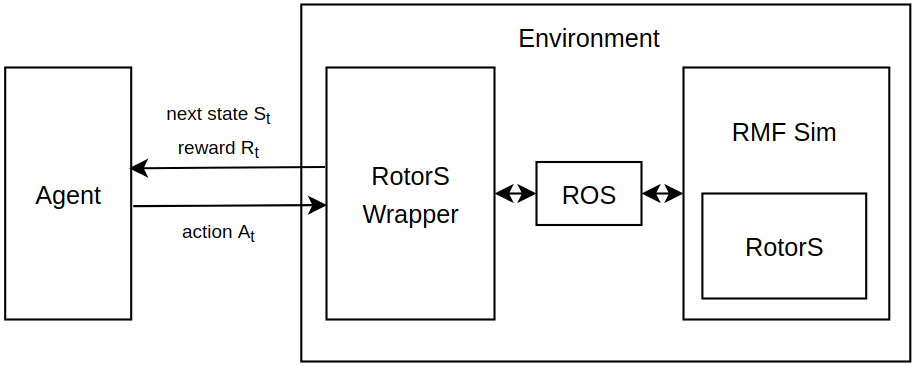
\includegraphics[width=0.85\textwidth]{figures/4_/4_1_simFramew.png}
    \caption{A diagram showing the overall simulation framework of our system, where different modules communicate via ROS.}
    \label{fig:4_1_simFramework}
\end{figure}


\subsection{ROS}
With the different components of the framework listed, what remains is the method of communication between these. The Robot Operating System (ROS) serves this purpose, being a middleware for robotics software \cite{ROS}. It is essentially a form of standardised communication, where different \textit{nodes} can communicate with each other, sending \textit{messages} via \textit{topics}. In this case, a node is simply an executable file that listens to or sends messages, by \textit{subscribing} and \textit{publishing} to a topic, respectively. A node can also offer a service, which will simply execute some function. 

ROS standardises the way that message passing occurs by using strictly typed data structures as messages which allows the type and content of a message to be easily identified. Similarly, topics are like message channels which allow us to quickly identify which nodes communicate with each other. These topics also allow new nodes to obtain messages it finds interesting by subscribing to those topics, without having to make any changes on the publisher side.

So, for this project, ROS is used as a way to integrate RotorS with the RMF module, but also as a method for the agent to communicate with the RMF Simulator, as seen in Figure \ref{fig:4_1_simFramework}.
In our case, the agent is directly able to communicate with the RotorS wrapper as they both exist in the same ROS package. 
The RotorS wrapper then serves as an environment interface, which receives odometry messages from, and sends thrust messages to, the RMF simulator.



\section{Experimental Setup}
\label{sec:4_5_experimentalSetup}

In this section, we go through the different design choices of the experiment, beginning with the reward function, before moving on the how the network is structured and how training is set up. Then, in Section \ref{sec:4_Experiment}, we will move on to the actual experiment of changing the \textit{hyperparameters} of the network and evaluating the effect this has on the performance of the DDPG and PPO algorithms.

\subsection{Reward Function}
\label{subsec:4_5_rewardFunction}

The reward function is one of the most important design tools within reinforcement learning. Through the choice of reward structure, one can indirectly manipulate the learned agent behaviour to match the behaviour we hope to observe during testing. Though conversely, having such a delicate tool may be a burden in disguise. The complex behaviour that an agent learns is based directly on the idea of maximising the total reward, by means of exploiting the environment, but also the reward function. Hence, any unmet expectations in the agent performance can often be the consequence of a poorly designed reward function.

For the purpose of waypoint navigation, we can construct a reward function that minimises the distance between the goal and the quadrotor, while  also maintaining a reasonable speed. We can add an additional goal reward to this function, which signals that the agent has been successful in reaching its goal.
The reward structure chosen is a quadratic reward function, inspired by the QP-problem formulation in optimal control. The reward function then resembles a cost function, penalising position, velocity and acceleration, with a goal reward $G$:
\begin{equation}
    R \, (S_t, A_t) = - S_t^\top \boldsymbol{Q} S_t -  A_t^\top \boldsymbol{R}  A_t  + G(S_t)
    \label{4_rewardFunction}
\end{equation}
Our states $S_t$ and actions $A_t$ are defined as in \eqref{4_1_stateActionsSpace} and the $\boldsymbol{Q}$ and $\boldsymbol{R}$ matrices represent the weighting for each element of the state and action. Explicitly, the reward can be written as:
\begin{equation}
R \, (\p_t, \v_t, \a_t) = - 
    \begin{bmatrix}
    x_t, y_t, z_t, 
    u_t, v_t, w_t
    \end{bmatrix}^\top
    \boldsymbol{Q}
    \begin{bmatrix}
    x_t\\
    y_t\\
    z_t\\
    u_t\\
    v_t\\
    w_t
    \end{bmatrix}
    -
    \begin{bmatrix}
    \Dot{u_t}, \Dot{v_t}, \Dot{w_t}
    \end{bmatrix}^\top
    \boldsymbol{R}
    \begin{bmatrix}
    \Dot{u_t}\\
    \Dot{v_t}\\
    \Dot{w_t}
    \end{bmatrix}
    + G(S_t)
\end{equation}
where,
\begin{equation}
    \boldsymbol{Q} = \frac{1}{250}
    \begin{bmatrix}
    0.6 & 0 & 0 & 0 & 0 & 0 \\
    0 & 0.6 & 0 & 0 & 0 & 0 \\
    0 & 0 & 1.0 & 0 & 0 & 0 \\
    0 & 0 & 0 & 0.03 & 0 & 0 \\
    0 & 0 & 0 & 0 & 0.03 & 0 \\
    0 & 0 & 0 & 0 & 0 & 0.05 
    \end{bmatrix}, \quad
    \boldsymbol{R} = \frac{1}{250}
    \begin{bmatrix}
    0.001 & 0 & 0 \\
    0 & 0.001 & 0 \\
    0 & 0 & 0.001
    \end{bmatrix}
    \label{4_QR_rewardWeights}
\end{equation}
and,
\begin{equation}
    G\,(S_t) =
    \begin{cases} 
      1 & \text{if} \,\, || \p_t || < 0.25 \,\, \text{and}\,\, || \v_t || < 0.3 \\
      0 & \text{otherwise}
    \end{cases}
    \label{4_goal_condition}
\end{equation}
Based on this reward function, the agent should be primarily motivated to reduce its position relative to the goal, but also with low speeds and without the use of excessive acceleration.
The goal reward serves the purpose to speed up the learning process, where it offers additional positive feedback so that the agent will know to repeat its actions. Further, we specify that the goal, $G(S_t)$, is reached if the quadrotor is able to stay within a goal radius of 0.25m with a total velocity of less than 0.3ms$^{-1}$. 

The weighting matrices $\boldsymbol{Q}$ and $\boldsymbol{R}$ describes the ``cost'' of each element, such that larger values correlate to more prioritised states and more expensive actions.
We can also note that the $z$ term is weighted more than the $x$ and $y$ terms in $\boldsymbol{Q}$. This choice is physically motivated by the fact that a quadrotor is more easily (directly) able to control its height rather than its lateral position, as shown in Section \ref{sec:4_2_dynamics}. Also, when considering that lateral accelerations require a change in the roll and pitch angles, this can result in unwanted changes to the quadrotor height. So, by having a more prioritised $z$ term, we wish that commanding the $\dot u$, $\dot v$ accelerations does not affect the height, $z$.

Another important consideration for the weighting matrices is that they should reflect the dynamics of the system. From \cite{song2021droneRacing}, we see that the inertial matrix for a quadrotor can be represented with a diagonal matrix $\boldsymbol{J} = [0.003, 0.003, 0.005]$ kg m$^2$, which is also provides a good justification for our chosen reward function.


\subsection{Network Architecture}
\label{sec:4_5_networkArchitecture}

In this section, we will look into the NN structure used for DDPG and PPO, and how these models are optimised. Recall from Chapter \ref{chap:3_Optimisation} that we can use NNs as function approximators that parametrise the policy $\pi$ and action-value function $Q$ (or value function $V$) in actor-critic algorithms.

\subsubsection{Network Types}
The most commonly used NN model is a fully-connected neural network (NN), which is also (ambiguously) referred to as a \textit{multi-layer perceptron} (MLP) in the reinforcement learning community. These models are the most conventional type of network, where each neuron in one layer is connected to every other neuron in the next layer.
There are also other model types that have been utilised, such as convolutional NNs (CNNs) in \cite{DQN}, or recurrent NNs (RNNs) like in \cite{Chen2016DRQN} that builds on \cite{DQN}. Generally, if we are dealing with structured data a CNN is most appropriate, while for data with a temporal relationship an RNN is beneficial. This being said, if our states hold the Markov property -- in contrast to partially observed MDPs (POMDPs) -- standard NNs are more than suitable as all the information in the previous states can be deduced from the current state.

\subsubsection{Network Choice}
So, in this project, we will be utilising fully-connected NNs to parametrise the policy and value functions. For DDPG, both networks have two hidden layers, where the width is a design parameter for this project, as described in Section \ref{sec:4_Experiment}. The Actor-Critic structure for DDPG is shown in Figure \ref{fig:4_3_networkArchitecture}. Note that for the DDPG algorithms, we have also target networks for both the actor and critic network with identical size, such that we have a total of four networks.
\begin{figure}[htb]
    \centering
        \begin{subfigure}[b]{.49\textwidth}
        \centering
        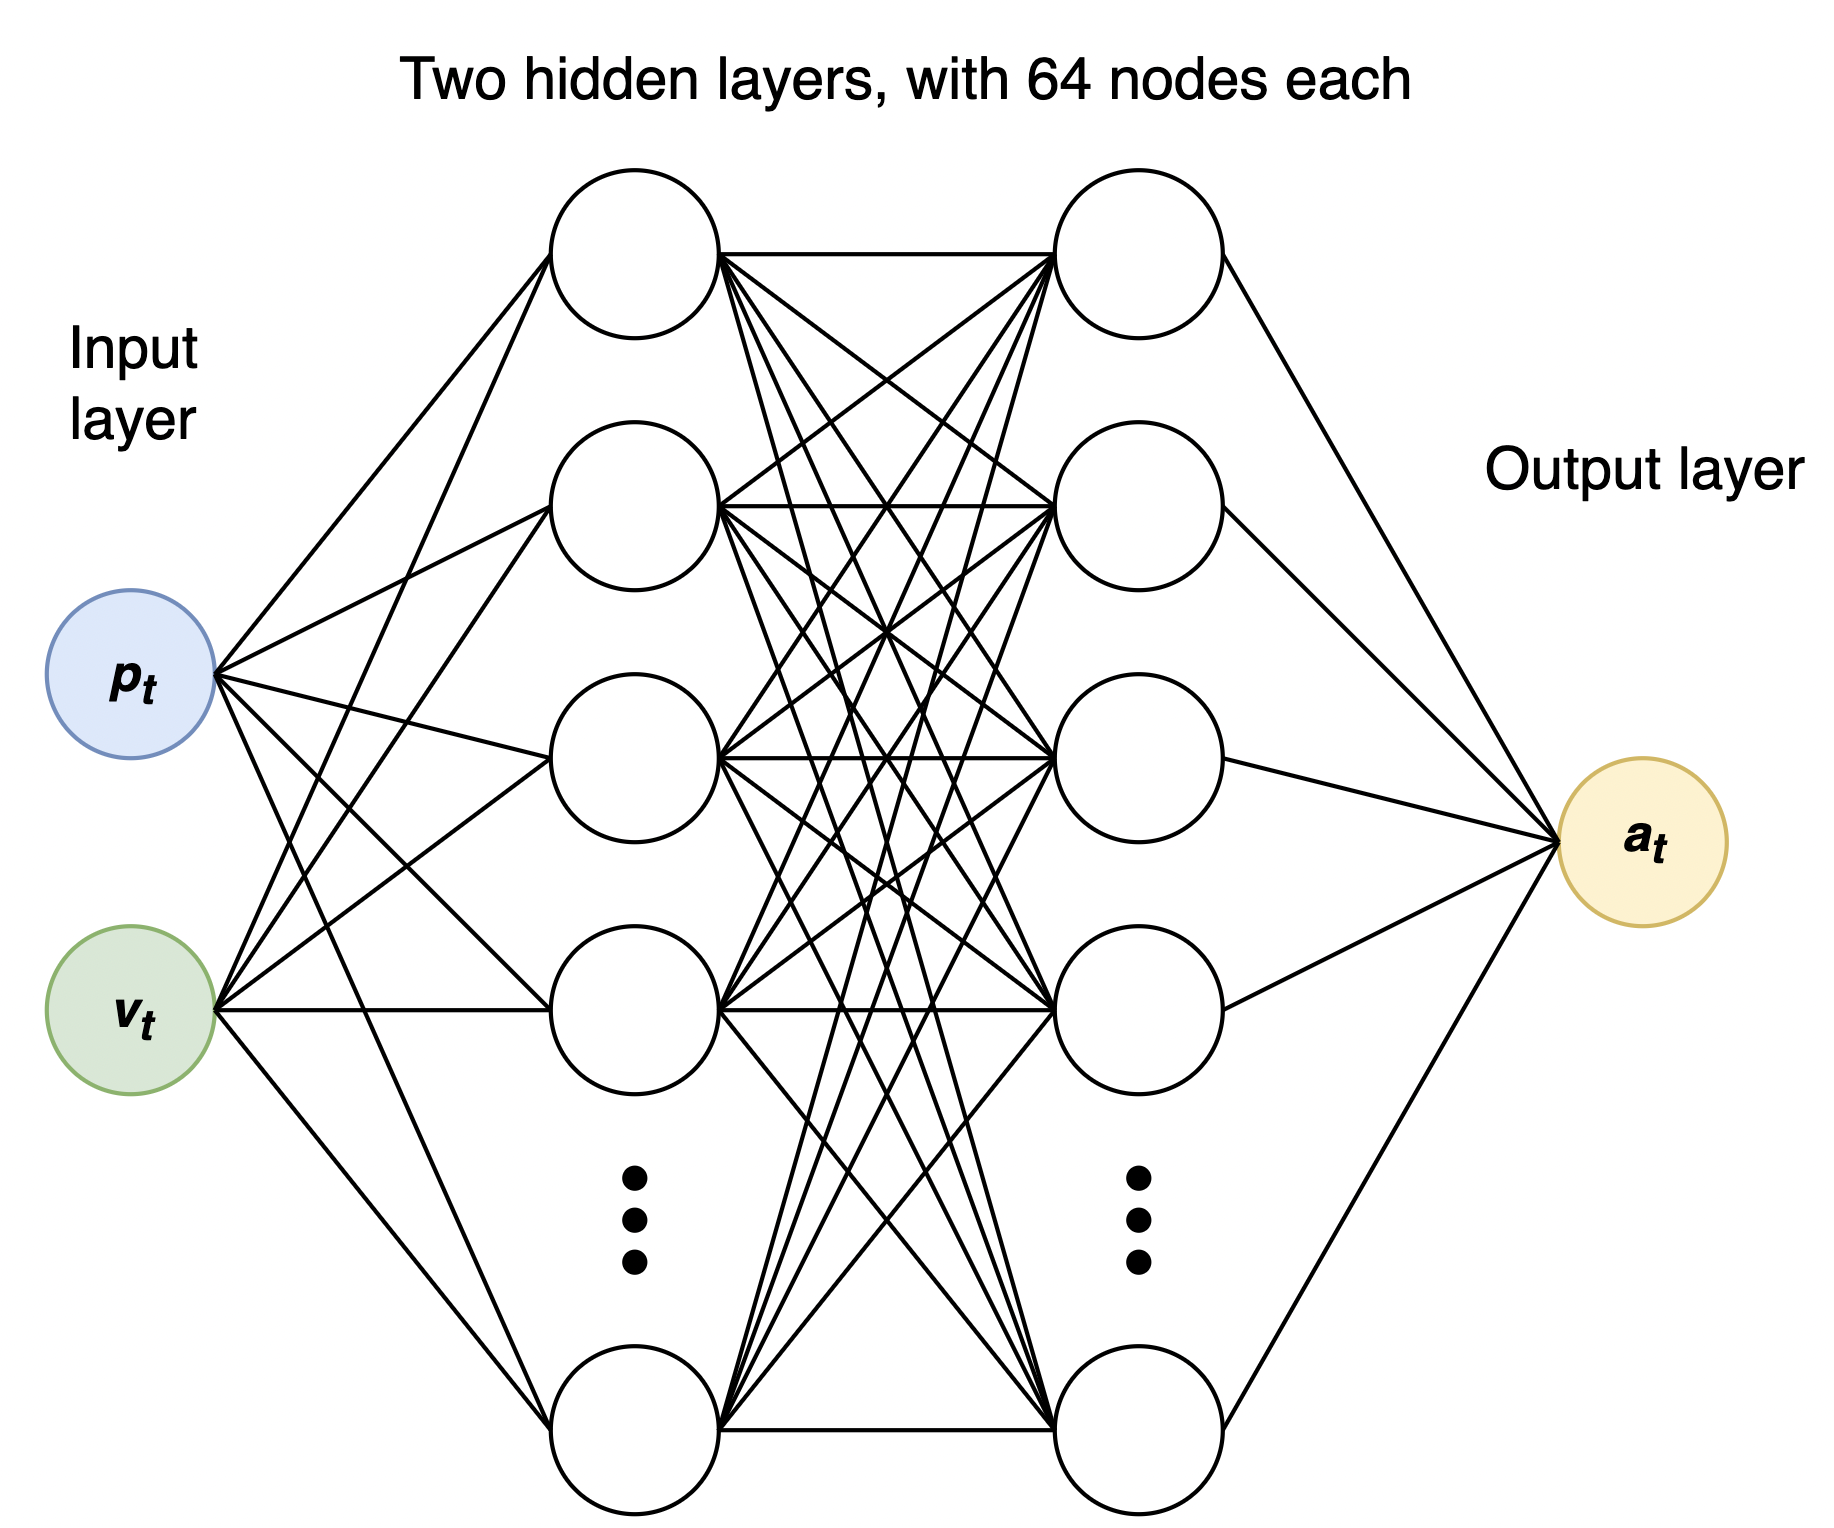
\includegraphics[width=.95\textwidth]{figures/4_/4_5_actor.drawio-labelled.png}
        \caption{Actor model with weights $\btmu$. The actor takes an input state $s \in \mathbb{R}^6$ comprising of a \textcolor[HTML]{004CD9}{position} $\p_t$ \textcolor[HTML]{009900}{velocity} $\v_t$ vector, to output an \textcolor[HTML]{D6C415}{acceleration} $\a_t  \in \mathbb{R}^3$ as action $a = \pi(s | \btmu)$.}
        \label{fig:4_3_actor}
    \end{subfigure}
    \hfill
    \begin{subfigure}[b]{0.49\textwidth}
        \centering
        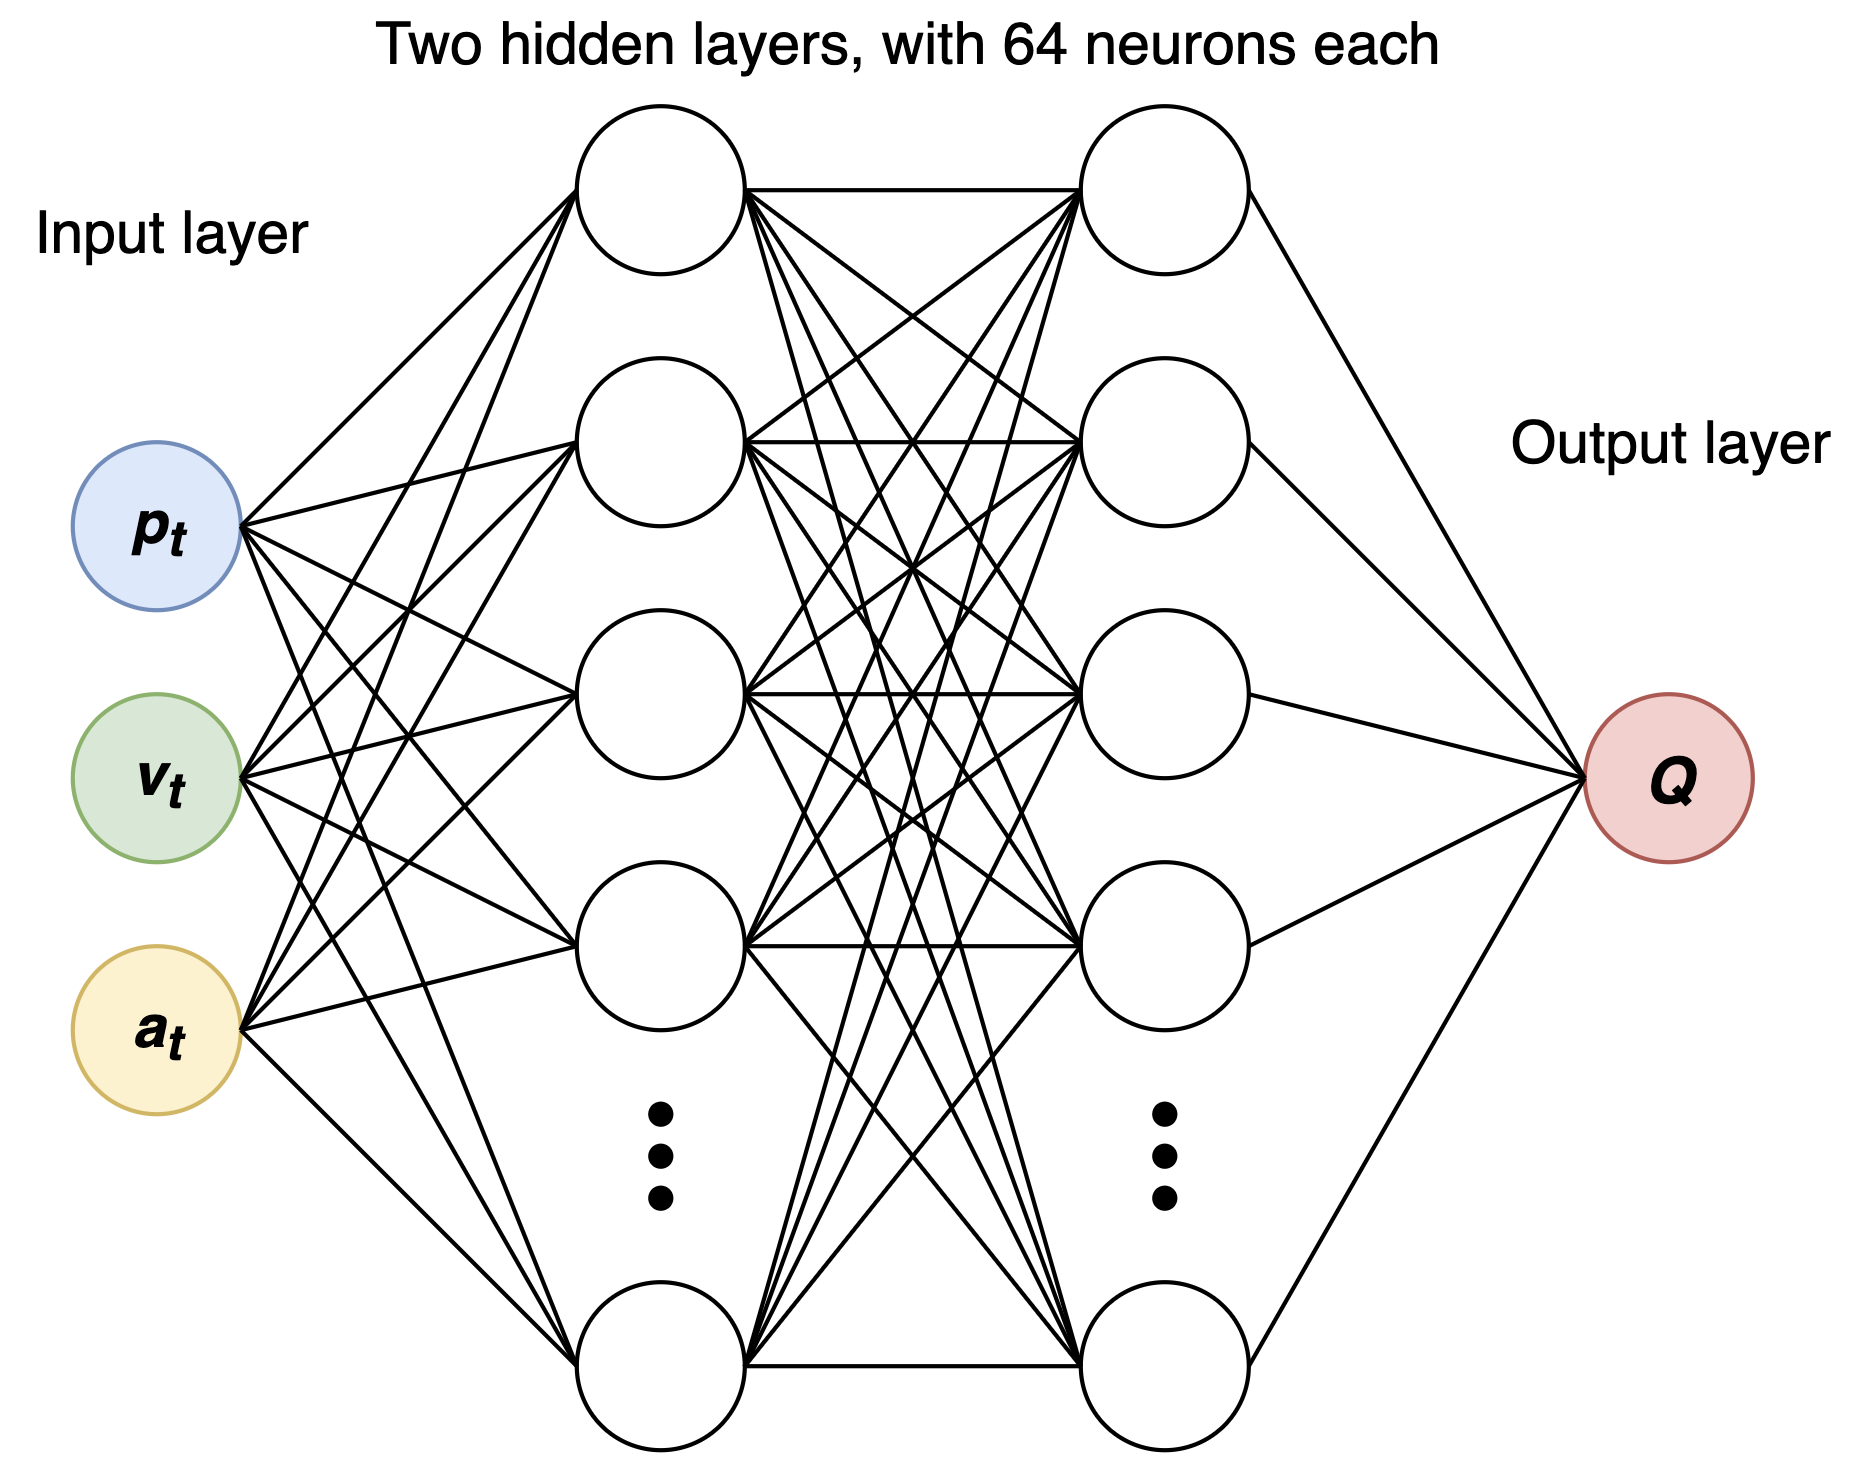
\includegraphics[width=.95\textwidth]{figures/4_/4_5_critic.drawio.png}
        \caption{Critic model with weights $\btQ$. The critic takes the concatenated state-action pair $[\p_t, \v_t, \a_t] \in \mathbb{R}^9$ as input, and yields the \textcolor[HTML]{CC262A}{estimated return} $Q(s,a | \btQ) \in \mathbb{R}$ for that pair, under some policy $\pi$.}
        \label{fig:4_3_critic}
    \end{subfigure}
    \hfill
    \caption{An overview of the actor and critic network architecture for DDPG.}
    \label{fig:4_3_networkArchitecture}
\end{figure}
\begin{figure}[hbt]
    \centering
        \begin{subfigure}[b]{.55\textwidth}
        \centering
        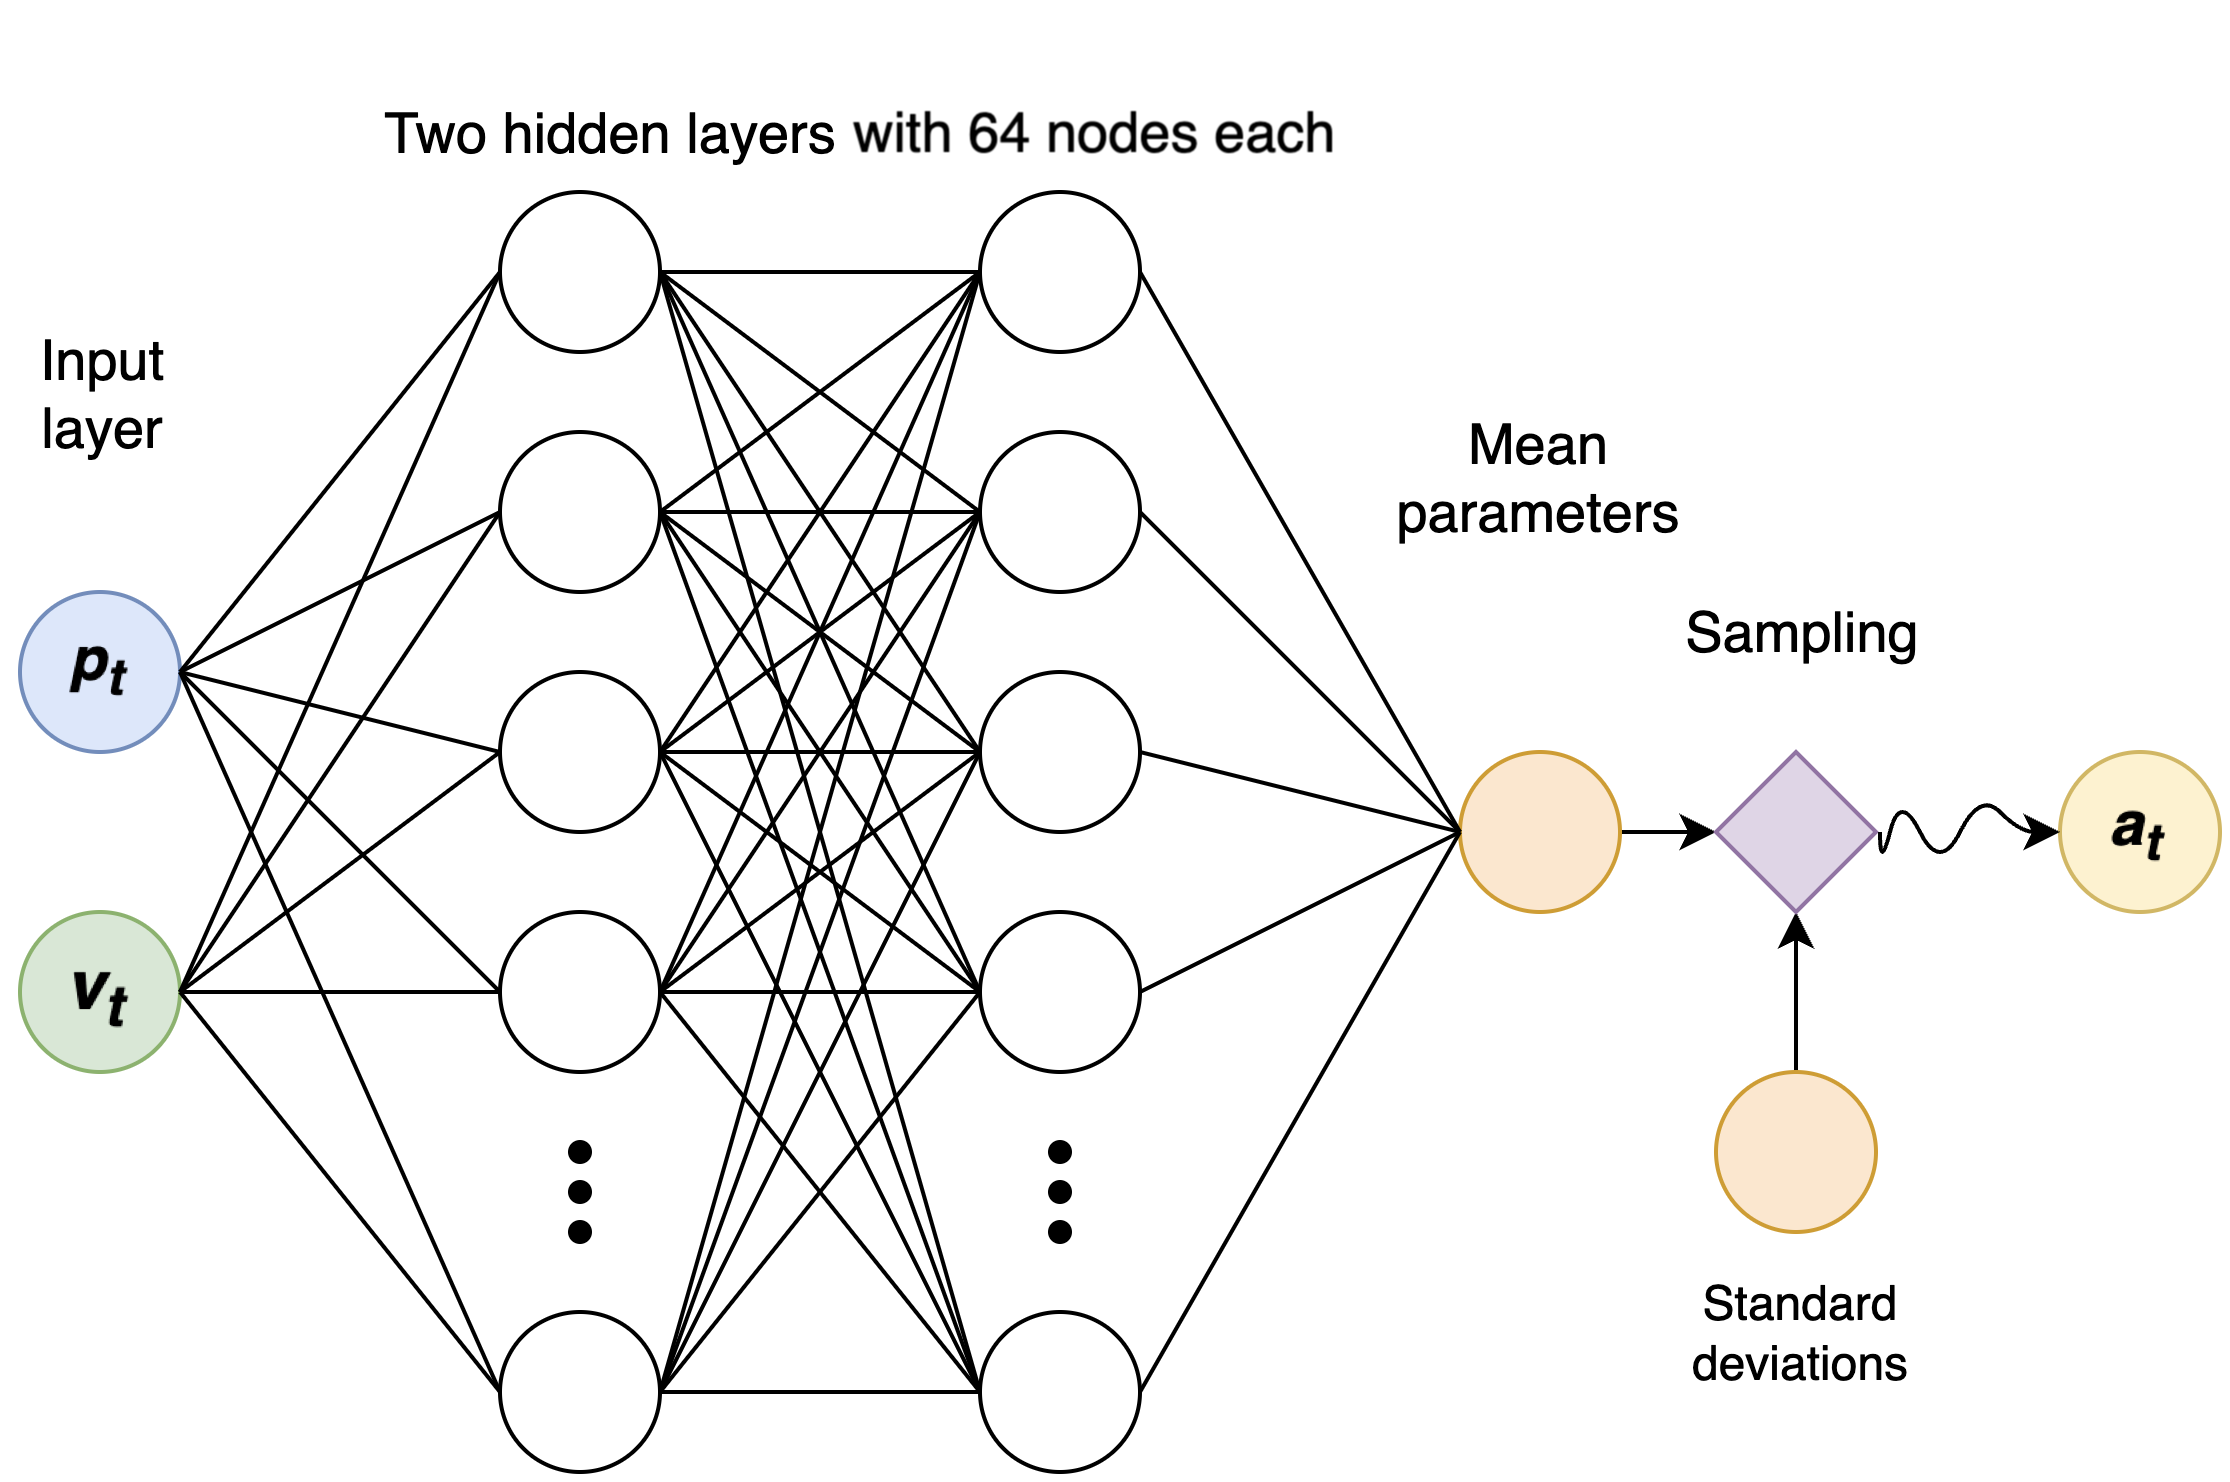
\includegraphics[width=.95\textwidth]{figures/4_/4_5_actor_ppo.drawio.png}
        \caption{Actor model with weights $\bt$, parametrising a stochastic policy $\pibt$. The actor takes an input state $s \in \mathbb{R}^6$ comprising of a \textcolor[HTML]{004CD9}{position} $\p_t$ \textcolor[HTML]{009900}{velocity} $\v_t$ vector, to output Gaussian distribution \textcolor[HTML]{DA8A67}{parameters} $\in \mathbb{R}^{3\times2}$, from which the \textcolor[HTML]{D6C415}{action} $\a_t \in \R^3$ is sampled.}
        \label{fig:4_5_PPOactor}
    \end{subfigure}
    \hfill
    \begin{subfigure}[b]{0.44\textwidth}
        \centering
        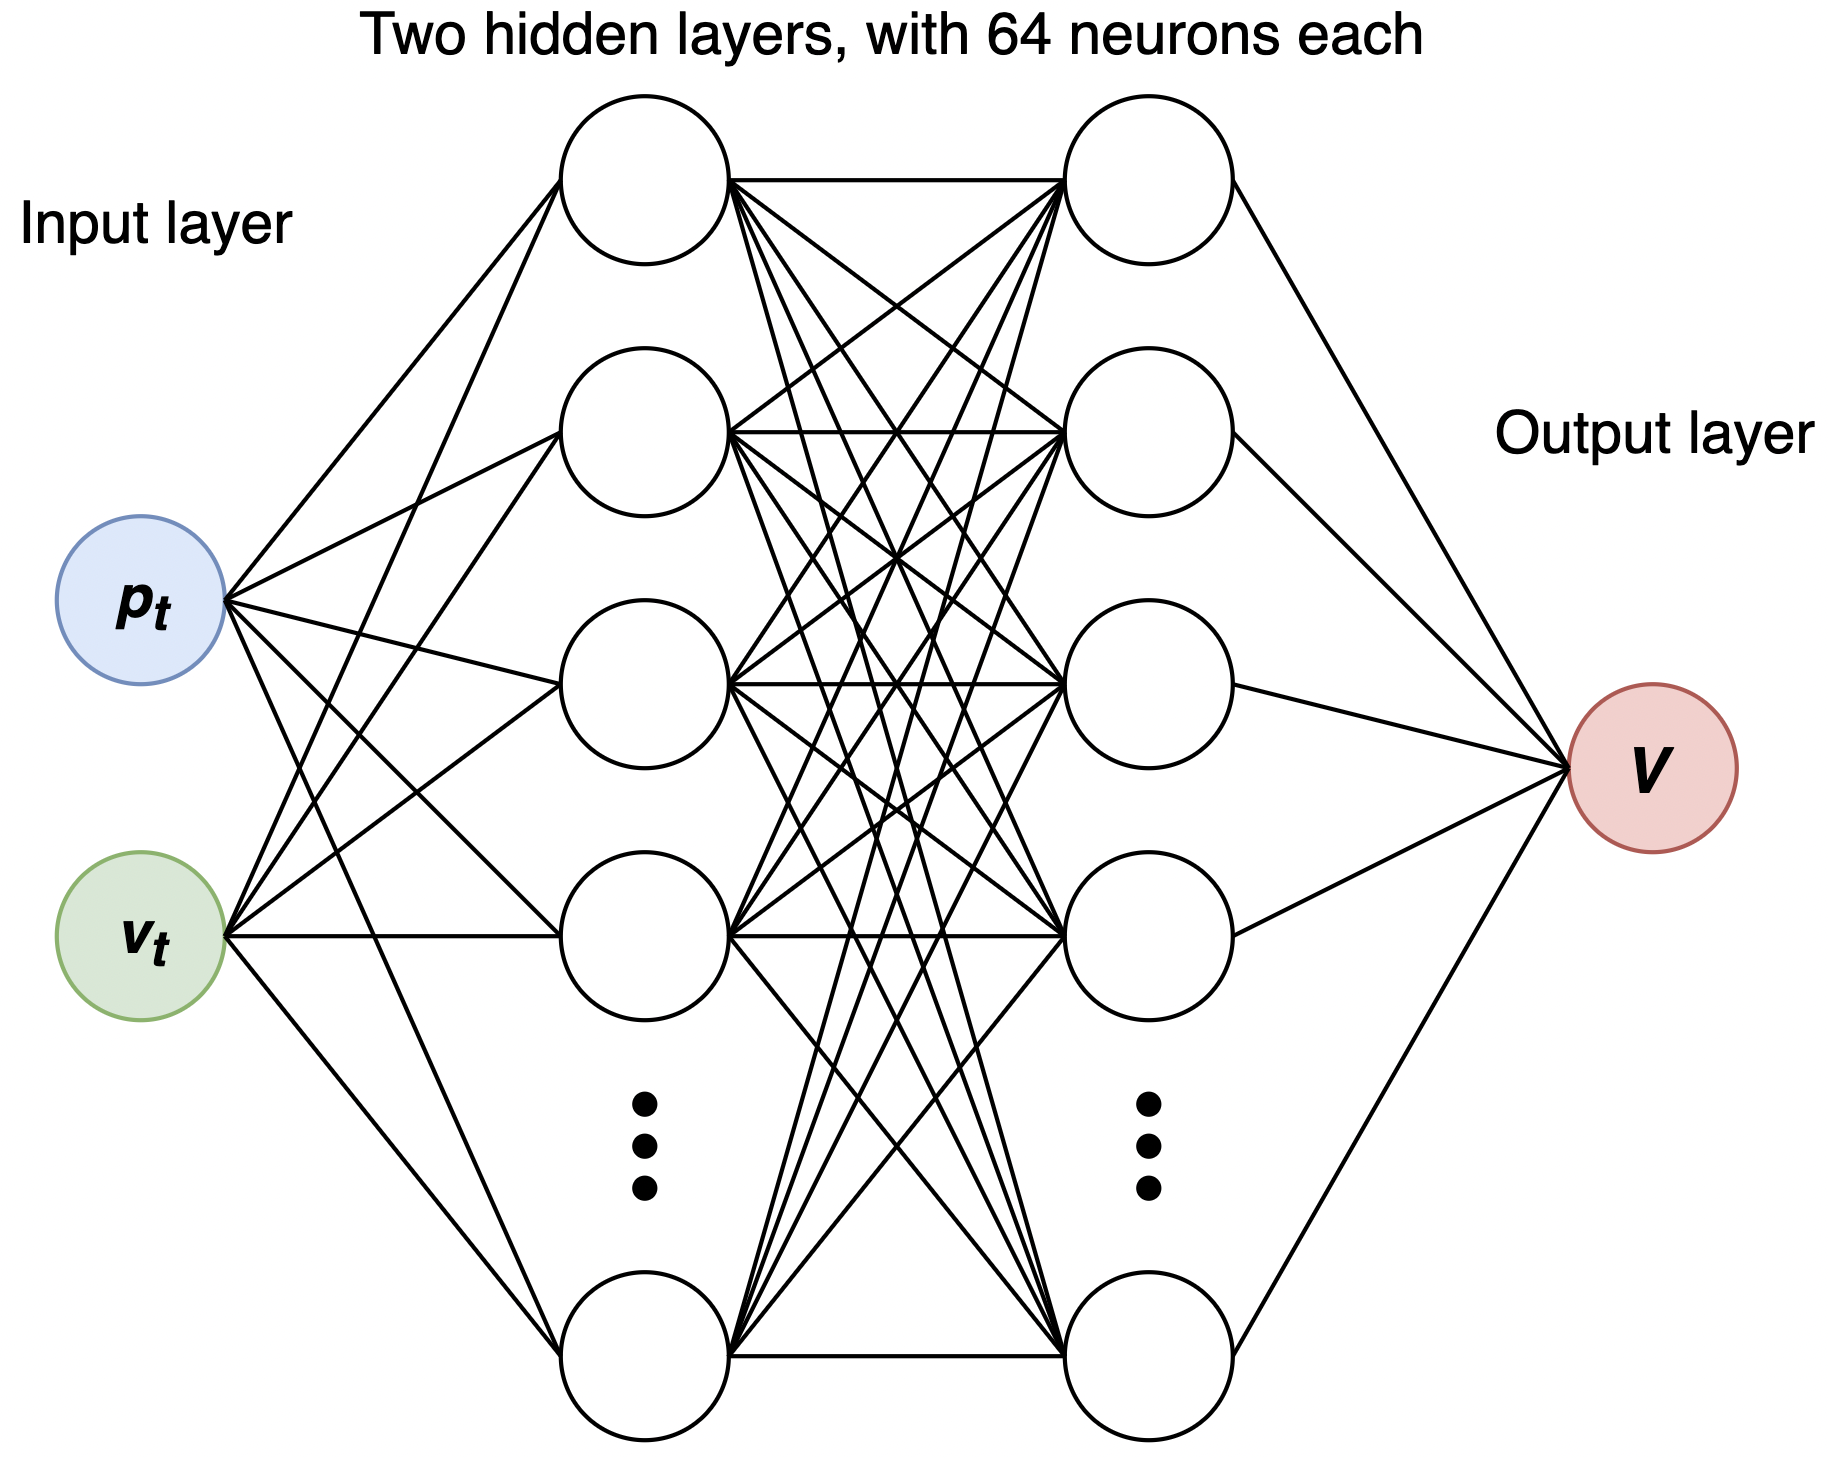
\includegraphics[width=.95\textwidth]{figures/4_/4_5_critic_ppo.drawio.png}
        \caption{Critic model also with weights $\bt$. The critic takes the state $[\p_t, \v_t] \in \mathbb{R}^6$ as input, to yield the \textcolor[HTML]{CC262A}{estimated return} $\Vbt \in \mathbb{R}$ for that state, under some policy $\pi$.}
        \label{fig:4_3_PPOcritic}
    \end{subfigure}
    \hfill
    \caption{An overview of the actor and critic network architecture for PPO.}
    \label{fig:4_3_PPOnetworkArchitecture}
\end{figure}

For PPO, the actor-critic structure is similar with two hidden layers, with 64 neurons in width. The actor differs slightly as we use a parametrised stochastic policy $\pibt$, such that the actions taken by the agent are sampled from the actor generated Gaussian distribution.
PPO also parametrises the value function $\Vbt$ for the critic, so that the critic network only takes in a state $s$ as input. 
The Actor-Critic structure for PPO is shown in Figure \ref{fig:4_3_PPOnetworkArchitecture}.

The choice of 64 neurons in each hidden layer of the network was primarily decided from results of previous projects at NTNU and seems to be supported by the literature \cite{ControlofQuadrotorRL, PPOQuadrotor, PPO}. Otherwise, other possible choices would be to double the width to 128 neurons, such as in \cite{song2021droneRacing}, or to use 200 and 100 neurons for the two hidden layers as in \cite{DDPG, RodriguezRamos2019ADR}. Otherwise, \cite{TRPO} uses fewer neurons with 30 or 20 in each layer depending on the task, with good results.

\subsubsection{Activation Functions}
As mentioned in Section \ref{subsec:DDPG_Innovations}, we need nonlinear activation functions to realise the generalisation potential of NNs. Therefore, we use a \textit{ReLU} activation function for each hidden layer, and \textit{tanh} activation function for the output layer. Further, the reason behind the use of tanh is that we wish use bound our acceleration $\a_t$ and Gaussian parameters outputs to a range $[-1,1]$. The reason why ReLU is used in the hidden layers, rather than the classic tanh in MLP implementations, is just a matter of preference in our opinion. 


\subsection{Training Setup}
\label{sec:4_5_trainingSetup}

With the network architecture decided, a critical phase of the method is how to train or optimise the NN model. As we are using the DDPG and PPO algorithms, the \textit{objective functions} or \textit{loss functions} for the actor-critic networks are already predetermined. We will instead focus on how to practical aspect of gathering experiences and data used for optimisation.

\subsubsection{Initialisation}
At the start of each run, the quadrotor is initiated at a random height between 8m and 10m, such that $S_0 = [0,0,z_0,0,0,0], \,\, z_0 \in [8, 10]$. For the goal position, we choose that $r = 3 * \sqrt[3]{c}$, where $c \sim [0,1]$. If the resulting goal position is less than 0.25m, we add 0.5m. Thus, we obtain a final radius of $r \in [0.25, 3.0]$ though the cube-root ensures that $r$ is much more likely near $3$.
From here, we set a timer such that the quadrotor has $3r$ seconds to reach the goal, or else the episode terminates. If the goal is reached, this is also regarded terminal state and the quadrotor and goal positions are reset. For reference, the timer allows roughly $120 \sim 180$ timesteps before timeout, depending on $r$.

\subsubsection{Gathering Experience}
An experience, in our case, is given by the set $\{S_t, A_t, R_t, S_{t+1} \}$ as mentioned in Section \ref{subsec:DDPG_Innovations}. For every timestep $t = 0,1,...T$, the quadrotor takes an action following its actor policy, lands in a new state, receives a reward, etc., and the accumulated experiences are then stored for later use. For DDPG, the experience is stored into a replay buffer $R$, while for PPO it is kept temporarily as a trajectory $T$. In the case of a terminal state, the quadrotor is reset but experience gathering continues normally. During training, noise is also added to the chosen actions in DDPG to assist with exploration, as discussed in Section \ref{subsec:3_4_DDPGactorCritic}.

\subsubsection{Gradient Updates}
To train a NN, gradient updates are usually made in \textit{batches} at the end of an \textit{epoch}. In this case, batches explicitly refers to collection of experiences of the quadrotor, randomly sampled from the replay buffer $R$ or trajectory $T$. 
When these gradient updates occur, or when the end of an epoch is, is a characteristic of the algorithm in question. 

For DDPG, epochs are less well-defined as updates are made after every timestep as seen in the pseudocode, Appendix \ref{app:algs_DDPG}. In practice, we follow the implementation from \cite{baselines}, where updates are made after every episode (cycle) instead. At the end of each episode, the gradients are calculated using batches are sampled uniformly over the replay buffer.
For PPO, a series of gradient updates are made after a trajectory has been sampled from the environment. We have defined this to be the end of an epoch, where $K$ gradient updates are made using minibatches created from this trajectory. This follows very closely from the PPO pseudocode in Algorithm \ref{alg:PPO_actorCriticStyle}, Appendix \ref{app:algs_PPO}.


\section{Experiment}
\label{sec:4_Experiment}

In this project, the approach for comparison between the DDPG and PPO algorithms will be through \textit{hyperparameter} testing. Through these tests, we aim to achieve a general understanding of the learning process behind these algorithms and their characteristics. Further, as we gain some understanding, we aim to learn how to tune these hyperparameters in order to obtain the best-performing agent. 

The experiment will be separated into two parts: first training, then testing. The idea is that models will be trained using a large combination of hyperparameters, such that we can select some of the decent performing models and analyse the effects of the different hyperparameters. In this phase, the primary criteria of evaluation will be on the highest \textit{average return} gained, along with the the number of training steps it requires.

Once a good set of trained models are selected for DDPG and PPO, we will then test them on a fixed waypoint navigation task with a constant waypoint.
This allows every model to be tested fairly and we can then compared the average reward per episode and the root-mean-squared error (RMSE) for each model. 

Finally, for the models with the best test results, we do an additional robustness test on the same fixed navigation task where the weight of the RMF quadrotor is altered by $\pm 10\%$. 


\subsection{Hyperparameters}
\label{subsec:4_6_hyperparameters}
As previously mentioned, the DDPG algorithm has been tested to an adequate degree in past projects here at NTNU. Therefore, we wish to compare the previously used models from master projects at NTNU with the baseline implementation in the original paper \cite{DDPG}. 
As a result, the DDPG hyperparameters that we will focus on are the:
\begin{itemize}
    \item Number of neurons in each hidden layer of the actor and critic networks -- i.e. the \textbf{network size},
    \item Actor and critic network \textbf{learning rates} $\boldsymbol{\alpha}$,
    \item \textbf{Size} of the \textbf{replay buffer} $R$.
\end{itemize}
This is not an exhaustive hyperparameter test, but we do focus on the most important aspects of the DDPG: the use of networks, the speed versus stability in learning, and the introduction of a replay buffer. Therefore, the results, albeit short, will be interesting nonetheless and can hopefully provide some insight into these hyperparameters.

Next, as the implementation of PPO was done alongside this project, there was a lot more uncertainty in what the ranges of these hyperparameters could be and how significant each of their effects were. Coupled with such a broad range of hyperparameters, there was a lot more room to explore what worked well and what did not. 
Therefore, we started by testing the original implementation of \cite{PPO}, and continued to experiment quite freely in the hyperparameter space.
The hyperparameters of interest are therefore:
\begin{itemize}
    \item \textbf{Size} of the \textbf{trajectory} $\boldsymbol{T}$,
    \item \textbf{Number of optimisation epochs} $\boldsymbol{K}$ per trajectory,
    \item \textbf{Number of minibatches }per trajectory, which determines the minibatch size $M$
    \item Actor and critic network \textbf{learning rates} $\boldsymbol{\alpha}$,
    \item \textbf{Coefficient} $\boldsymbol{c_1}$ of the value function loss term $J_t^{VF}(\bt)$,
    \item \textbf{Coefficient} $\boldsymbol{c_2}$ of the entropy term $S[\pi_{\bt}](s)$
\end{itemize}
As we can see, all the hyperparameters are algorithm hyperparameters specific to PPO. To get a quick refresher of these hyperparameters, one can refer to the pseudocode in Appendix \ref{alg:PPO_actorCriticStyle} and sections \ref{subsec:PPO-clip} and \ref{subsec:3_ppo_actorCritic}. 

So since we did not have a implementation for quadrotor guidance to compare it to and needed to infer all hyperparameters ourselves. As a result, as we will see in the the following chapters, the project therefore also puts more emphasis on testing the PPO algorithm.
\chapter{Results}
\label{chap:results}
\begin{comment}
Results
Some plots
Rewards - loss - RMSE

We choose some models, to reflect the \textbf{hyperparameters} choices (Magnus does reward). Use "best performance" regardless of number of runs and 

Summarise best results, based on hyperparameters and under what controls (reward, goal setting, rules idk) also vs. the baseline (paper or OpenAI release) implementation. 

Do this separately for DDPG and PPO, internal competition, then compare best of the two. 

Can we generalise results based on some hyperparameters? Can we come to conclusions on others? Don't over-complicate. 

3 robustness tests for PPO, 2 for DDPG
Results in excel,
\end{comment}

\section{Overview}

In this chapter, we will present the results for the DDPG and PPO algorithms. This will include a presentation of some of the selected models for each algorithm, where we look at the effect of hyperparameters in the training process and the overall performances during testing. Lastly, the best models are tested again with $\pm10\%$ mass to evaluate their robustness.

To visualise the results, we have the training graphs for each model. These include one for \textit{average return}, \textit{actor loss} and \textit{critic loss}. The average return will be our standard performance metric for the agent, while the loss analysing the loss curves will provide information about the actor-critic networks. We also provide the model training times, run on an Intel(R) Core(TM) i7-8700 CPU @ 3.20GHz processor.

For the fixed waypoint tests, a goal point is initialised at roughly $[1.84, 1.84, 1.5]$ meters away, or exactly at a point with $r=3$m with relative angles $\psi=45\degree$ and $\theta = -30\degree$. 
\begin{figure}[hbt]
    \centering
    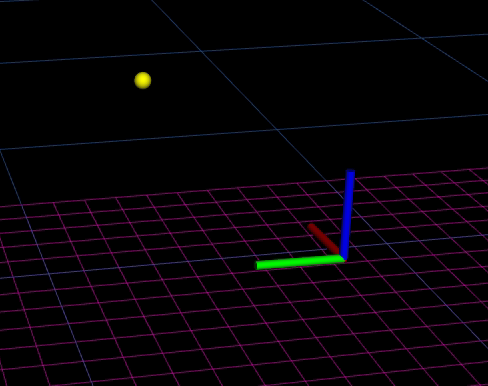
\includegraphics[scale=0.8]{figures/5_/5_waypoint.png}
    %\captionsetup{justification=centering}
    \caption{The goal seen with a yellow marker with $\p_0 = \approx [1.84, 1.84, 1.5]$.The quadrotor body frame is shown as \textcolor{red}{x}, \textcolor{green}{y}, \textcolor{blue}{z}.}
    \label{fig:5_waypoint}
\end{figure}
This is calculated through $x = r \sin{\theta}  \cos{\psi}, \,\,y = r \sin{\theta}  \sin{\psi}$ and $z = r \cos{\theta}$.

With this, each model will then attempt to fly to this goal marker 100 times and we compute the root-mean-squared cross-track error (RMSE) and average return per episode, averaged across all episodes. The cross-track error is calculated by finding the perpendicular distance to the quadrotor from a point on the shortest path (line) to the goal.
Additionally, for select scenarios we distinguish models further by plotting a typical run, such that we can see the quadrotor flight trajectories and can analyse its response.

\section{DDPG}
\label{sec:5_DDPG}

The DDPG models chosen for testing are shown in Table \ref{table:4_6_DDPG_hyperparameters}.
\begin{table}[hbt]
    \centering
    \begin{tabular}{||M{3.5cm}||M{3cm}|M{3cm}|M{2cm}||}
    \hline
    \centering
    Model & Network size & Learning rate, $\alpha$ & Buffer size \\ \hline\hline
    Previous NTNU & 64, 64       & 1e-5, 1e-5                           & 1e5            \\ \hline
    Original & 200, 100     & 1e-4, 1e-3                           & 1e6            \\ \hline
    Modified & 64, 64       & 1e-4, 1e-3                           & 1e5            \\ \hline
    \end{tabular}
    \caption{The different DDPG models tested, along with their hyperparameters. The size 200, 100 refers to the sizes of the first and second hidden layers, while the rate 1e-4, 1e-3 are the learning rates for the critic and actor respectively.}
    \label{table:4_6_DDPG_hyperparameters}
\end{table}
To explain the names, the ``Previous NTNU'' model is the model that was implemented in previous projects here at NTNU, while the ``Original'' one denotes the baseline implementation by \cite{DDPG}. In addition, the ``Modified'' model is chosen to illustrate a good combination of hyperparameters from the Previous NTNU and Original models.

\subsection{Training}
\label{sec:5_ddpg_training}
The training of these models are done as described in Section \ref{sec:4_5_trainingSetup}. For DDPG, we found that the models required a significant amount of training time to achieve a good performance.
\begin{table}[hbt]
    \centering
    \begin{tabular}{||M{3cm}|M{3cm}|M{4cm}||}
    \hline
    \centering
    Model & Epoch & Training time \\ \hline\hline
    NTNU     & 1452 & 18h 4m  \\ \hline
    Original & 1792 & 21h 25m \\ \hline
    Modified & 1500 & 17h 44m \\ \hline
    \end{tabular}
    \caption{The time used to train each of the DDPG models presented.}
     \label{table:5_trainingTime_DDPG}
\end{table}
We have selected the last epoch as the best epoch for each of these models, based from the training curves seen in Figure \ref{fig:5_training_DDPG}.
\begin{figure}[H]
     \centering
     \begin{subfigure}[b]{0.78\textwidth}
         \centering
         \captionsetup{justification=centering}
         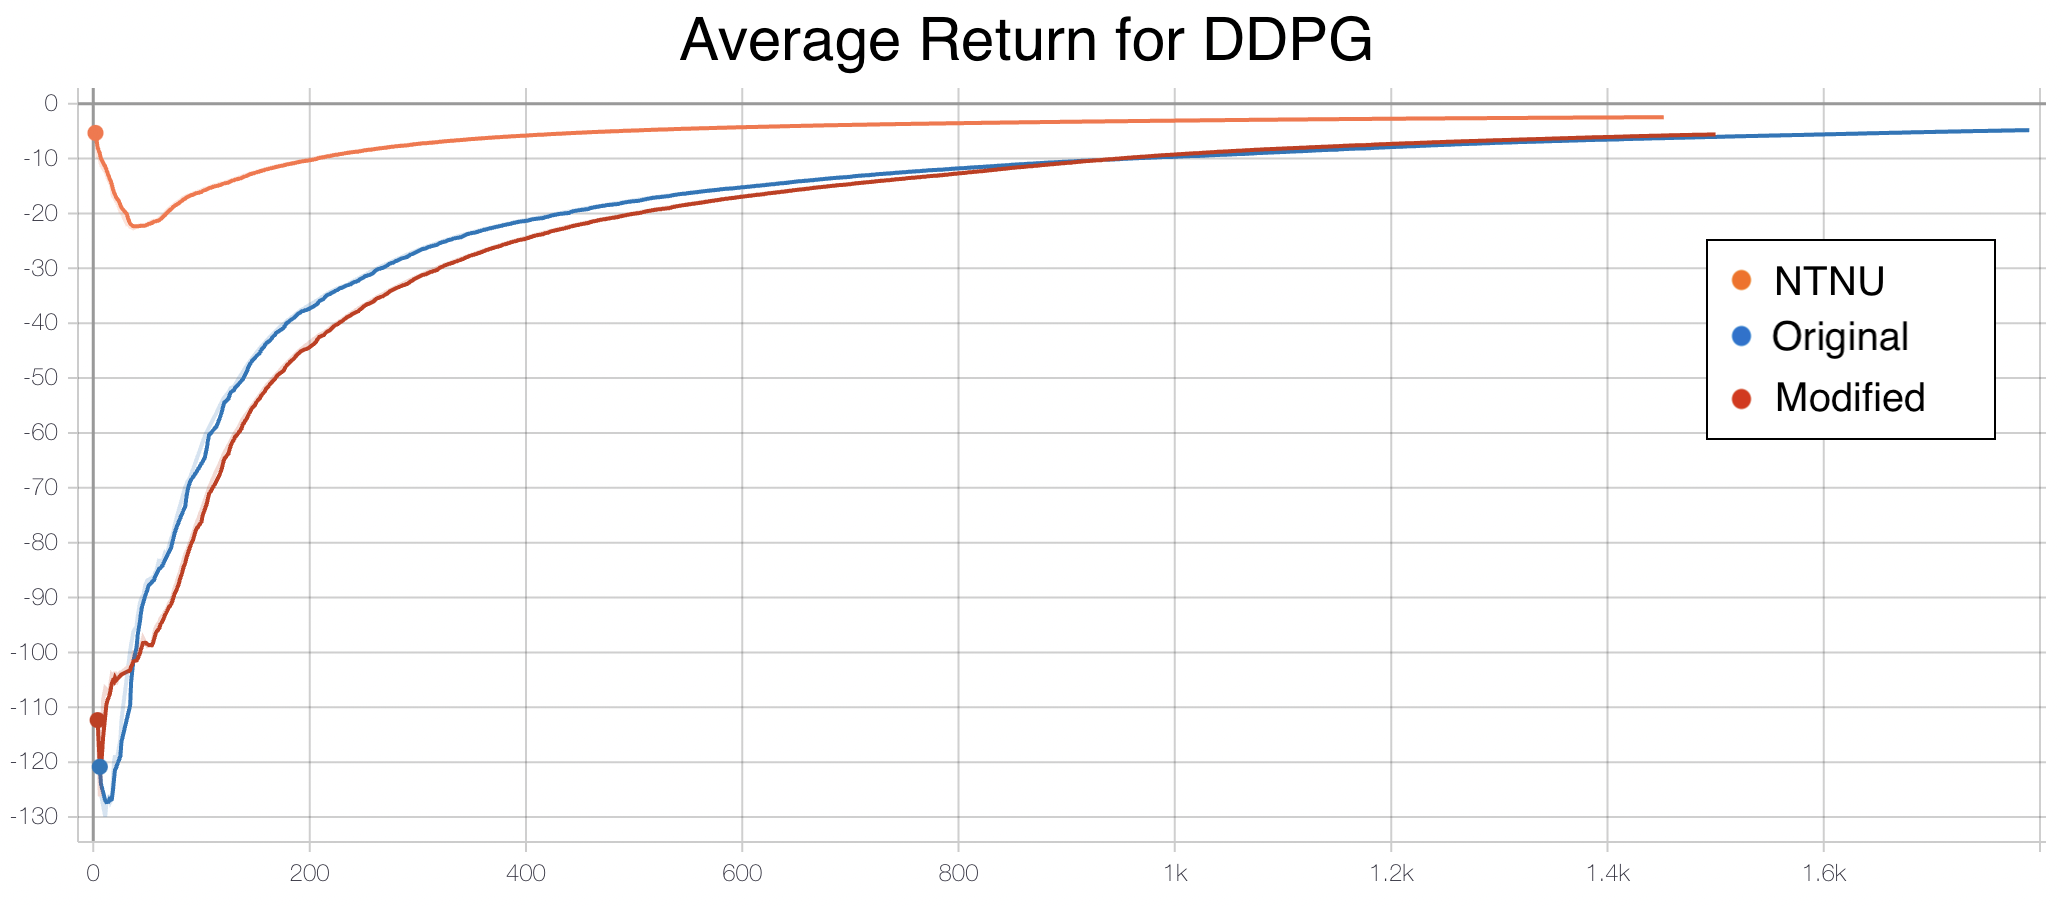
\includegraphics[width=\textwidth]{figures/5_/Training/ddpg_return.png}
         \caption{Average return for the three DDPG models, where the return is averaged across all previous episodes.}
         \label{fig:training_ddpgReturn}
     \end{subfigure} 
     \hfill \\[5mm]
     \begin{subfigure}[b]{0.78\textwidth}
         \centering
         \captionsetup{justification=centering}
         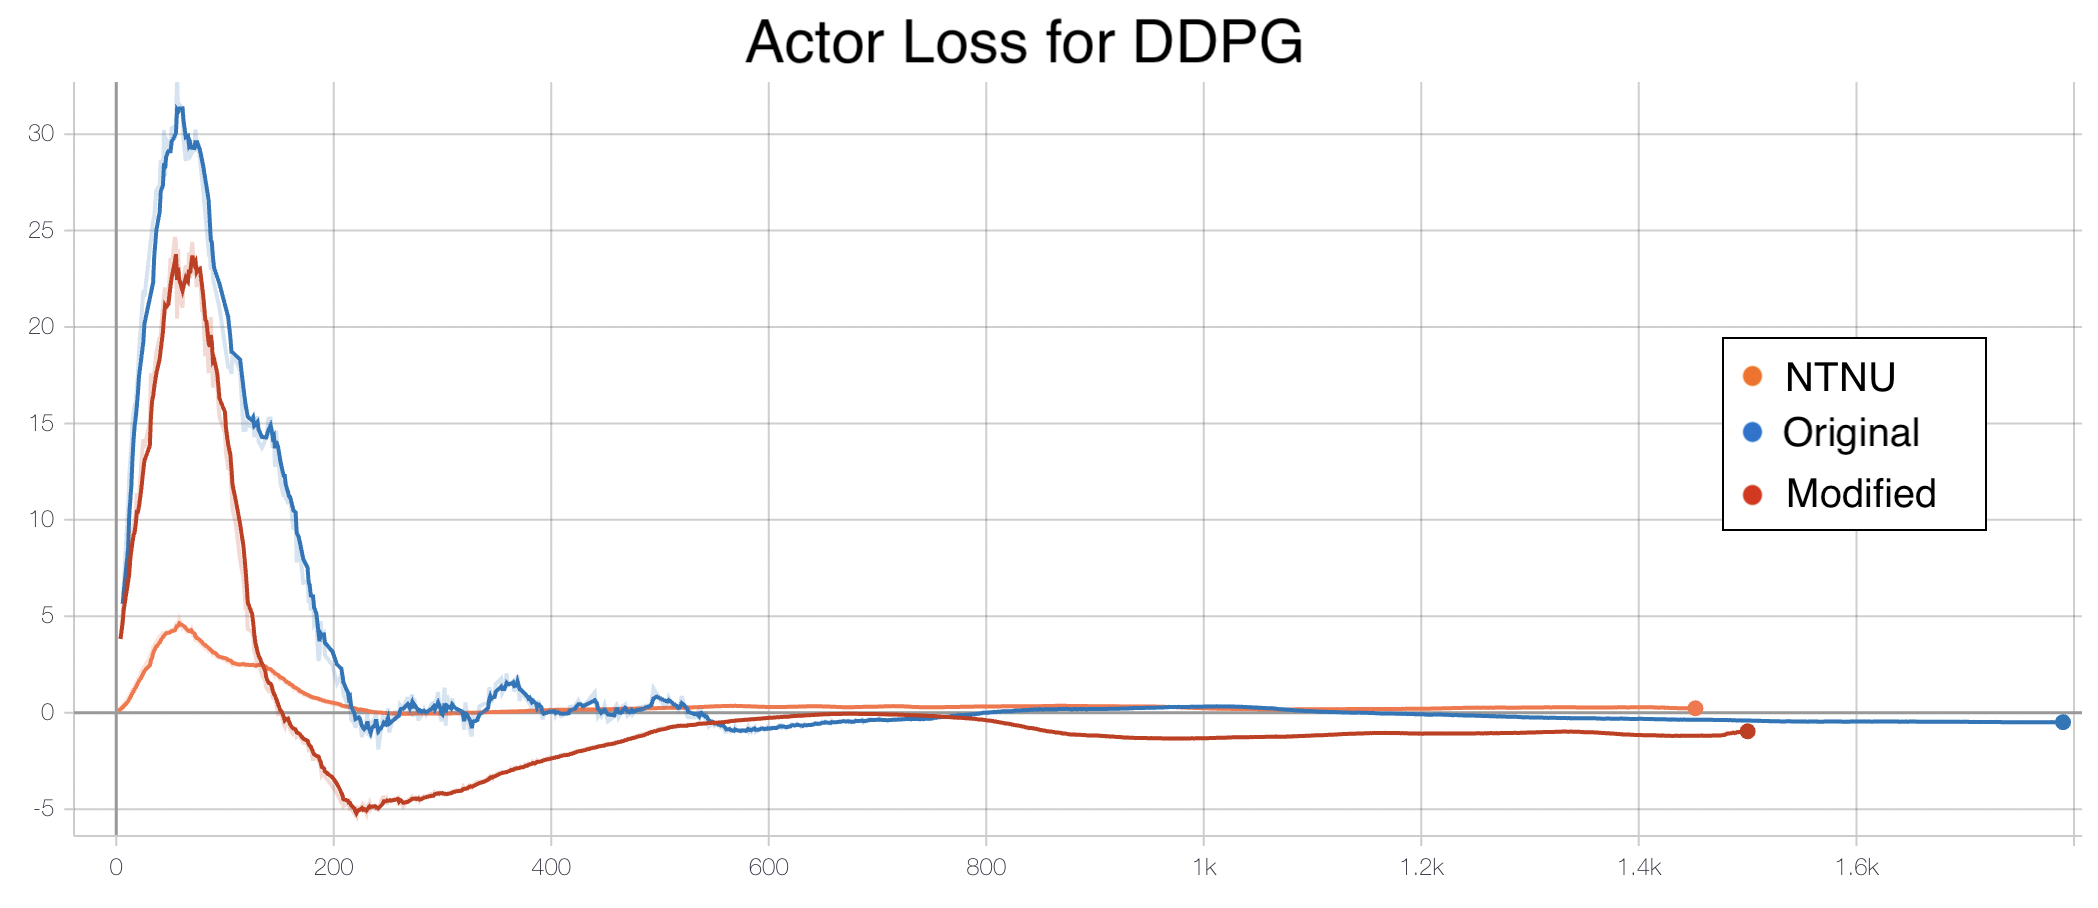
\includegraphics[width=\textwidth]{figures/5_/Training/ddpg_actorLoss.png}
         \caption{The actor loss of the DDPG models per epoch, given by the \textit{negative} of the actor objective function, $\Qt$, as seen in Equation \eqref{3_4_actorLoss}.}
         \label{fig:training_ddpgActorLoss}
     \end{subfigure}
     \hfill \\[5mm]
     \begin{subfigure}[b]{0.78\textwidth}
         \centering
         \captionsetup{justification=centering}
         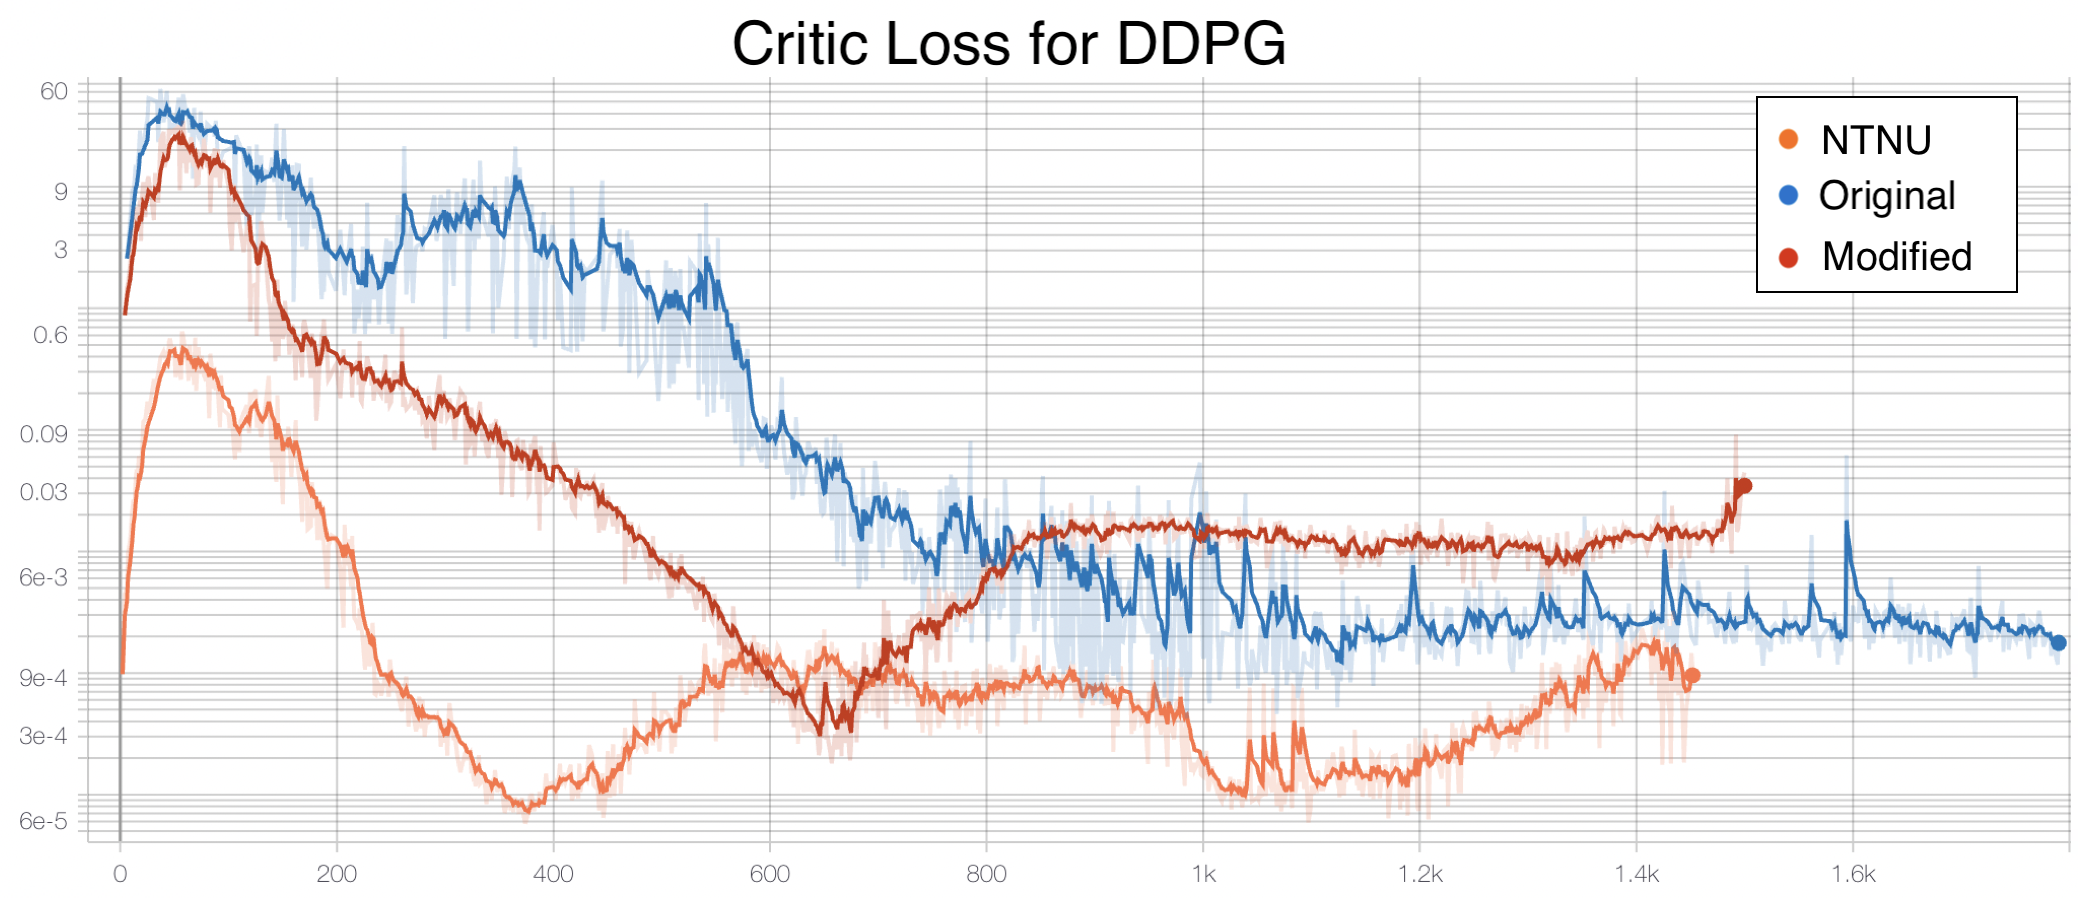
\includegraphics[width=\textwidth]{figures/5_/Training/ddpg_criticLoss.png}
         \caption{The critic loss of the DDPG models per epoch. The loss is the MSE of the estimated Q-value and the target Q-value, shown in Equation \eqref{3_4_criticLoss}. Note the log $y$-axis.}
         \label{fig:training_ddpgCriticLoss}
     \end{subfigure}
    \captionsetup{justification=centering}
    \caption{The training process for the three DDPG models. The $x$-axis shows the number of epochs the model is trained for where an epoch is 20 episodes.}
     \label{fig:5_training_DDPG}
\end{figure}
Looking at the Figure \ref{fig:5_training_DDPG}, we observe that the Previous NTNU model has the highest average return, with the Original and Modified models practically identical. For reference, at the end of their training, each model had an average return of -2.45, -4.80, -5.58 respectively.
We should also note that the average return curve is surprisingly smooth. This is because the average return is the mean return over all previous episodes and not the 20 episodes of that particular epoch. Arguably, this could be a design flaw in hindsight. So knowing this, the actual value of the average return for a certain epoch may be misleading of the agent's performance, and actually, it is not clear to see which model is performing best amongst the three. 

Therefore, we can instead look at the actor-critic loss curves. Beginning first with the actor loss in Figure \ref{fig:training_ddpgActorLoss}, we can see that by roughly 700 epochs all the values settle at 0. However, we then see that both the Modified and the Original loss curves converge to negative loss values, which initially might appear strange if we think about its definition (describing a negative error?).
Yet, since the actor loss is actually just the \textit{negative} of the estimated return $\Qt$, we should understand the actor loss as DDPG's method of predicting the actor performance. This makes sense since a high actor loss means very negative expected return and bad performance, while a low actor loss means high expected return which is a good performance. 

However, the $\Qt$ value is merely a prediction. To gauge its accuracy, we turn to the critic loss. Given by Equation \eqref{3_4_criticLoss}, the critic loss is the MSE of the target Q-value and its current prediction, corresponding to the prediction error $\overline{VE}$ in Section \ref{sec:3_3_actor-critic}. 
So, as the critic loss approaches 0, the target critic and critic networks essentially are in agreement throughout the episode, which only happens if DDPG does well to predict its Q-value for each state of the episode. So, this is means that a \textit{low critic loss} is an indication of consistently \textit{accurate critic Q-value} predictions.
From Figure \ref{fig:training_ddpgCriticLoss}, we see that all critic losses approach 0 relatively quickly, such that by epoch 750 all losses are below 0.01.
From epoch 800 onwards, the losses flatten, which shows low rates of learning and is a good indication that we can trust the Q-values. 

This means that by reading the actor loss again, we see that from epoch 1000, the best model is in fact the Modified model, which predicts the highest (negative) average return for each epoch. Then the Original model follows second, which has a higher estimated return compared the Previous NTNU model, seen at epoch 1500.
As for the hyperparameters, we can attribute the difference in training largely to the significantly larger learning rates, which transforms the worst model, the Previous NTNU one, into the best model in roughly the same amount of training epochs. We also note that having a larger network size and buffer size does not improve training in this example, though this is not conclusive.

\subsection{Testing}
\label{sec:5_ddpg_tests}
Now that we analysed the training data of these models, we can now test these models and see if the test data concurs with our analysis. The results for our three models on the fixed goal task is given in Table \ref{table:5_DDPG_tests}.
\begin{table}[hbt]
    \centering
    \begin{tabular}{||M{2cm}||M{2.5cm}|M{3.5cm}|M{2.5cm}||}
    \hline
    Model & Goal Rate & Average Return & Average RMSE \\\hline\hline
    NTNU     & 0      & -6.539     & 0.170    \\\hline
    Original & 96      & -0.040     & 0.042    \\\hline
    Modified & 98      & -0.704     & 0.029 \\\hline
    \end{tabular}
    \caption{The test results for the DDPG models, averaged over 100 episodes.}
    \label{table:5_DDPG_tests}
\end{table}

From this table, we observe that the Modified model reached the goal most often at 98\% success, followed by the Original at 96\%. We also note that the Previous NTNU model was not able to reach the goal at all at its point in training. We also see from the Modified model is consistently taking the shortest path to goal among the three models, seen through the low RMSE. 

Very unexpectedly, however, we observe that the average return for the Modified model is much less than the Original model, contradicting the results of the goal rate and average RMSE. To know for sure, we can take a look at the last test run for both models in Figure \ref{fig:5_testing_DDPG}.
\begin{figure}[H]
     \centering
     \begin{subfigure}[b]{0.51\textwidth}
         \centering
         \captionsetup{justification=centering}
         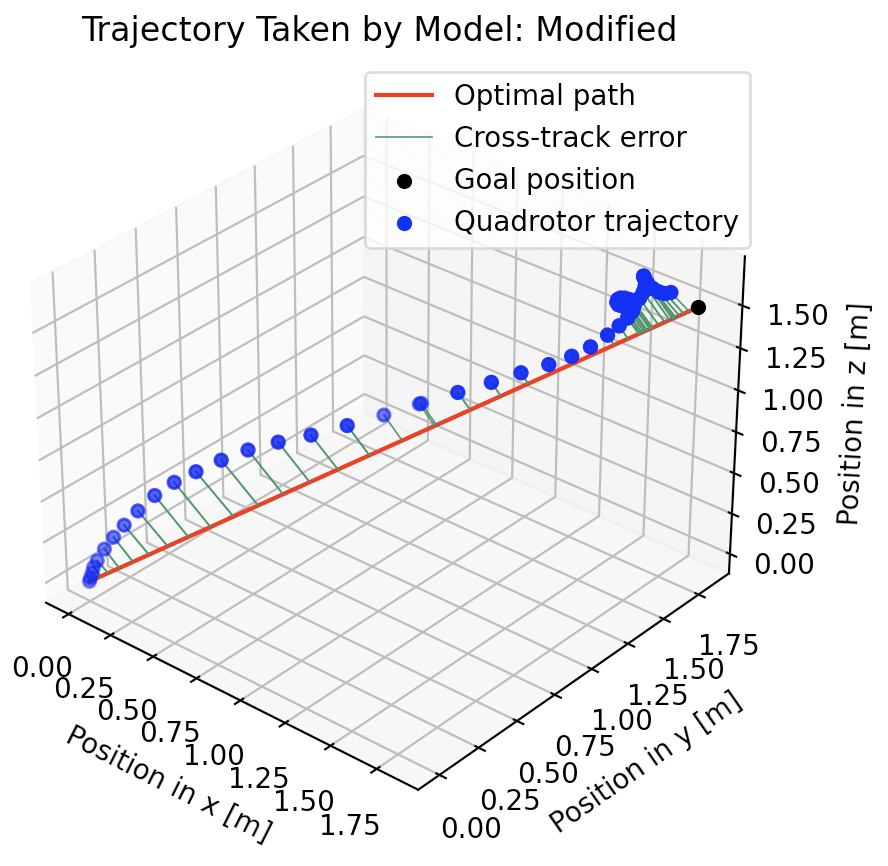
\includegraphics[width=\textwidth]{figures/5_/Testing/ddpg_test_modified1.png}
         \caption{The trajectory of the quadrotor with the Modified model compared to the shortest path.}
         \label{fig:testing_ddpgModified1}
     \end{subfigure} 
     \hfill 
     \begin{subfigure}[b]{0.48\textwidth}
         \centering
         \captionsetup{justification=centering}
         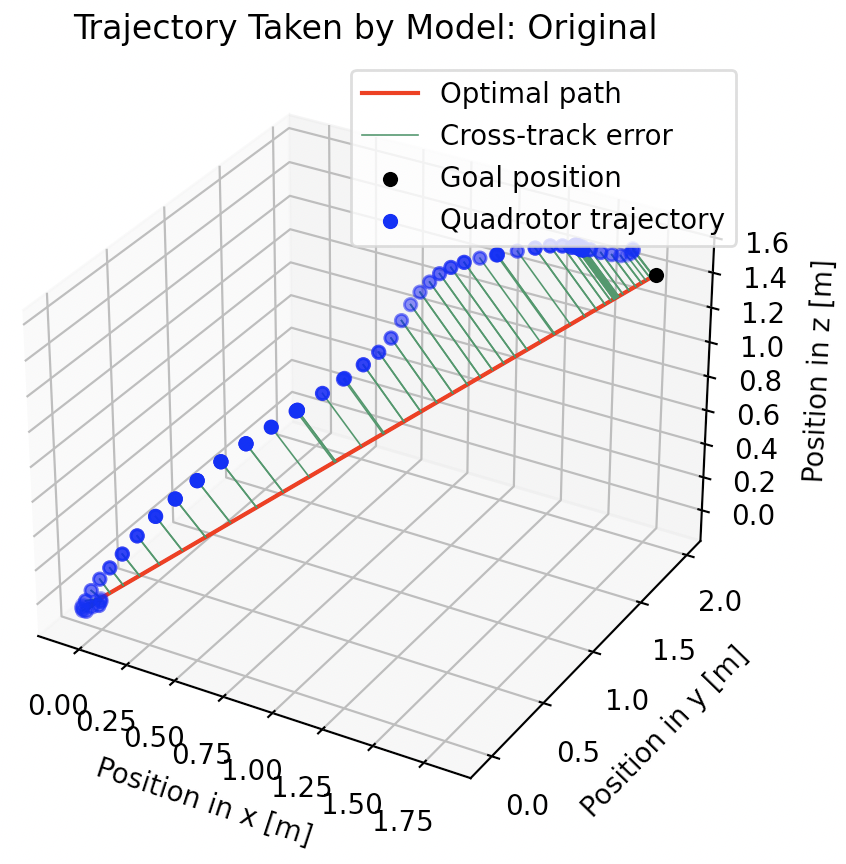
\includegraphics[width=\textwidth]{figures/5_/Testing/ddpg_test_original1.png}
         \caption{The trajectory of the quadrotor with the Original model compared to the shortest path.}
         \label{fig:testing_ddpgOriginal1}
     \end{subfigure} 
     \hfill \\[10mm]
     \begin{subfigure}[b]{0.49\textwidth}
         \centering
         \captionsetup{justification=centering}
         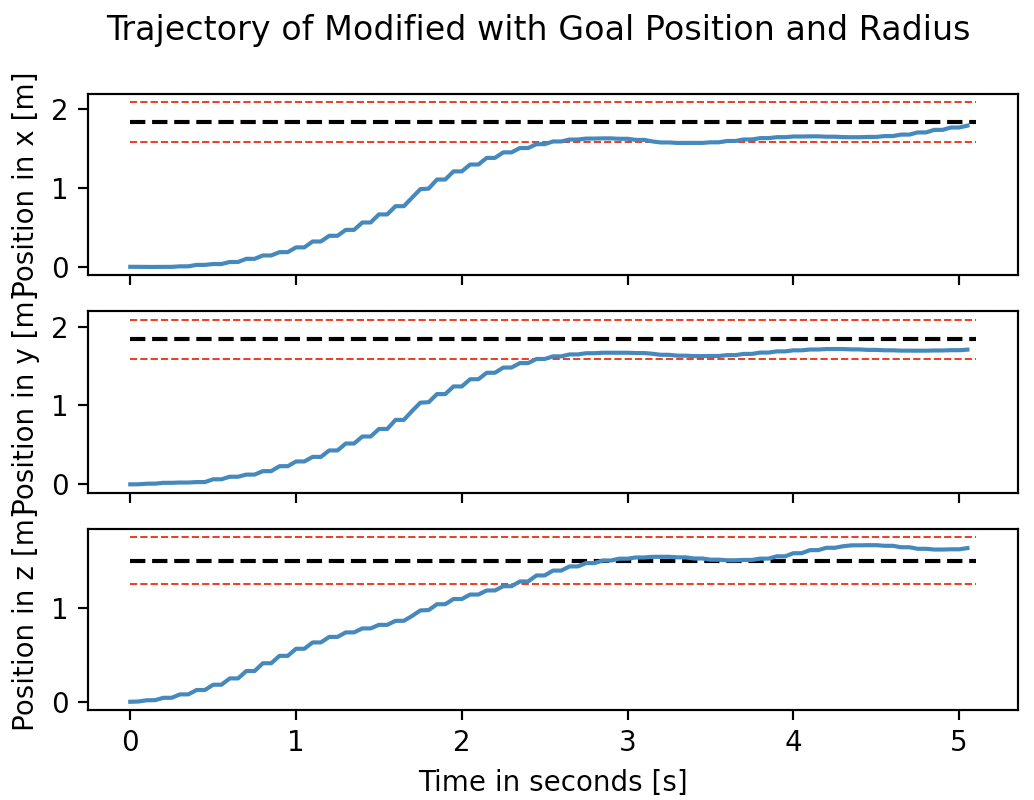
\includegraphics[width=\textwidth]{figures/5_/Testing/ddpg_test_modified2.png}
         \caption{The trajectory of the quadrotor with the Modified model compared to the goal position, decomposed in $x$, $y$, $z$.}
         \label{fig:testing_ddpgModified2}
     \end{subfigure} 
     \hfill 
     \begin{subfigure}[b]{0.49\textwidth}
         \centering
         \captionsetup{justification=centering}
         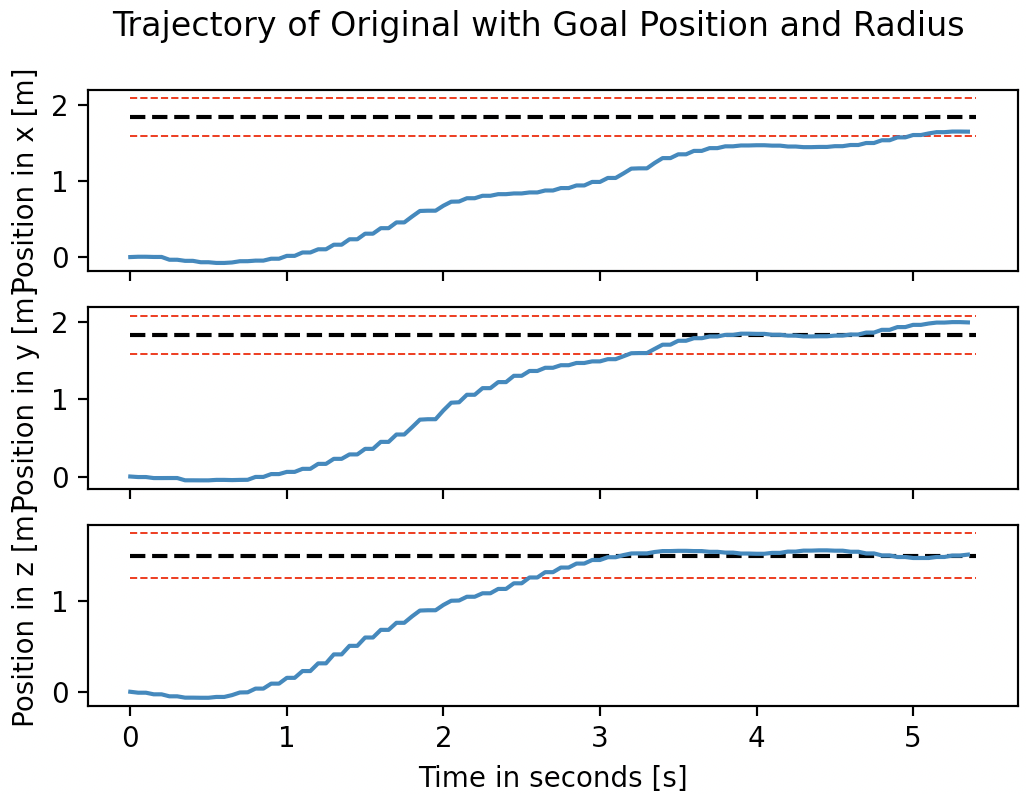
\includegraphics[width=\textwidth]{figures/5_/Testing/ddpg_test_original2.png}
         \caption{The trajectory of the quadrotor with the Original model compared to the goal position, decomposed in $x$, $y$, $z$.}
         \label{fig:testing_ddpgOriginal2}
     \end{subfigure} 
    \captionsetup{justification=centering}
    \caption{Test run no. 100 for the Modified and Original DDPG models.}
     \label{fig:5_testing_DDPG}
\end{figure}
From Figures \ref{fig:testing_ddpgModified1} and \ref{fig:testing_ddpgOriginal1}, it is clear that the Modified model performs best, with the smallest cross-track error over the whole episode and matching the result given in Table \ref{table:5_DDPG_tests}. This result is further highlighted in subplots (c) and (d), where the Modified run is significantly outperforms the Original in the $x$-axis, with similar performance in $y$ and $z$. We see also that the quadrotor is within the goal region at about 3 seconds in the Modified model, while it takes about 5 seconds to reach the same goal region for the Original model. The reason that the episode does not terminate earlier for the Modified model, is probably due to its more aggressive response. In (a), the we can see that the spacing is marginally wider than that in (b), showing a greater speed. We can therefore guess that the overall speed $||\v_t|| > 0.3$, such that we do not satisfy our goal condition in \eqref{4_goal_condition}. In contrast, when the Original controller reaches the goal region, the episode terminates instantly, which tells us that a gentle approach is made towards the goal. 

Nonetheless, the higher $\v_t$ is not significant enough to cause such a difference in the average return. Instead, our guess is that the average return for the Modified model in \ref{table:5_DDPG_tests} is actually an error. To take a closer look at this, both models were checked to see which episodes did not result in a goal. Interestingly, episode 7 was disastrous for the Modified model, seen in the table below:
\begin{table}[H]
    \centering
    \begin{tabular}{||c||c|c||}
    \hline
    \multicolumn{3}{||c||}{Episode Data for Test Runs no. 7 and 51} \\
    \hline\hline
        Episode Total squared-error & 5799.8317 & 286.0620 \\ 
        Episode steps & 181 & 181  \\
        Episode RMSE & 0.4208 & 0.0934\\
        Episode Return & -88.259 & -8.367 \\
    \hline
    \end{tabular}
    \caption{Failed test runs no. 7 and 51 for the Modified DDPG model. Note the large episode RMSE and return, compared to that in Table \ref{table:5_DDPG_tests}.}
    \label{tab:5_DDPG_errorTestRun}
\end{table}
Test run no. 7 was a significant anomaly in the test data, even when compared to run 51. Therefore in my opinion, it is more insightful and beneficial to neglect these in the comparison. So, by taking into consideration only the test runs that resulted in a reaching the goal state, we obtain Table \ref{table:5_DDPG_adjustedtests}.
\begin{table}[hbt]
    \centering
    \begin{tabular}{||M{2cm}||M{2.5cm}|M{2.5cm}|M{2.5cm}||}
    \hline
    Model & Goal Rate & Average Return & Average RMSE \\\hline\hline
    NTNU     & 0      & -6.539     & 0.170 \\\hline
    Original & 100    & 0.183      & 0.037   \\\hline
    Modified & 100    & 0.267      & 0.025
     \\\hline
    \end{tabular}
    \caption{The adjusted test results for the DDPG models, where 4.}
    \label{table:5_DDPG_adjustedtests}
\end{table}
From this table, we see that the adjusted test results are now all in agreement with each other, and we obtain an average return which reflects the goal bonus of +1 much more clearly.


\subsubsection{Robustness Test with $\pm10\%$ Mass}
\label{sec:5_ddpg_robustnessTests}
The last result that we have is the robustness test results for when the quadrotor mass is altered by a factor 0.1. With our simulated RMF weighing 500g, this was an additional or removed 50g. For this test, only the Original and Modified models were tested. The results are shown in Table \ref{table:5_DDPG_robustnesstests}.
\begin{table}[hbt]
    \centering
    \begin{tabular}{||M{2.3cm}||M{2.5cm}|M{2.5cm}|M{2.5cm}||}
    \hline
    Model & Goal Rate & Average Return & Average RMSE \\\hline\hline
         \textbf{+10\% Mass} &           &            &          \\\hline
Original & 0      & -1.414     & 0.039    \\\hline
Modified & 7      & -1.019     & 0.025   \\\hline\hline
         \textbf{-10\% Mass} &           &            &          \\\hline
Original & 0      & -65.841    & 0.595    \\\hline
Modified & 0      & -63.652    & 0.318  \\\hline
    \end{tabular}
    \caption{The robustness test results for the DDPG models, averaged over 100 episodes.}
    \label{table:5_DDPG_robustnesstests}
\end{table}
\begin{figure}[H]
     \centering
     \begin{subfigure}[b]{0.51\textwidth}
         \centering
         \captionsetup{justification=centering}
         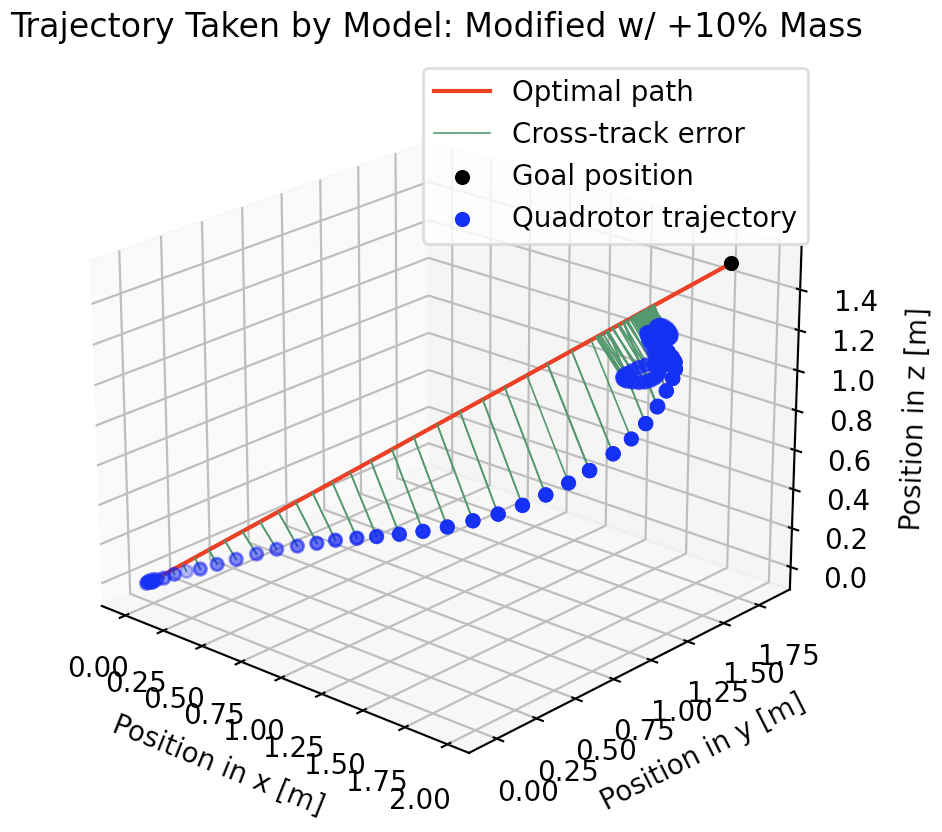
\includegraphics[width=\textwidth]{figures/5_/Testing/ddpg_test_robust+10-1.png}
         \caption{The trajectory of the quadrotor with +10\% mass, under guidance of Modified.}
         \label{fig:ddpg_test_robust+10-1}
     \end{subfigure} 
     \hfill 
     \begin{subfigure}[b]{0.48\textwidth}
         \centering
         \captionsetup{justification=centering}
         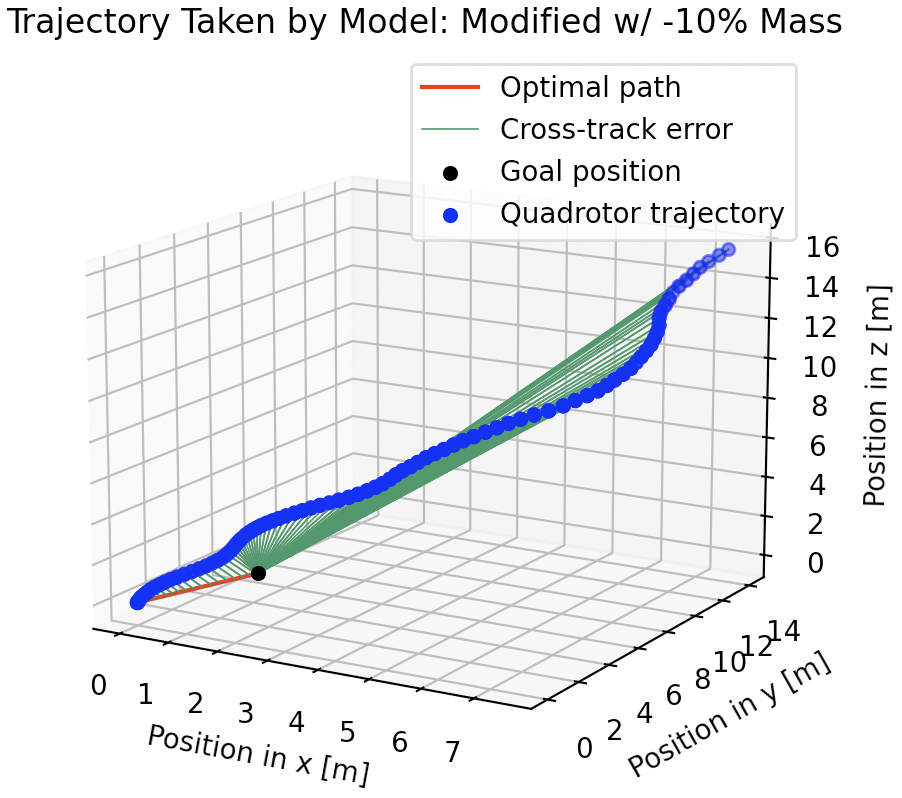
\includegraphics[width=\textwidth]{figures/5_/Testing/ddpg_test_robust-10-1.png}
         \caption{The trajectory of the quadrotor with -10\% mass, under guidance of Modified.}
         \label{fig:ddpg_test_robust-10-1}
     \end{subfigure} 
     \hfill \\[10mm]
     \begin{subfigure}[b]{0.49\textwidth}
         \centering
         \captionsetup{justification=centering}
         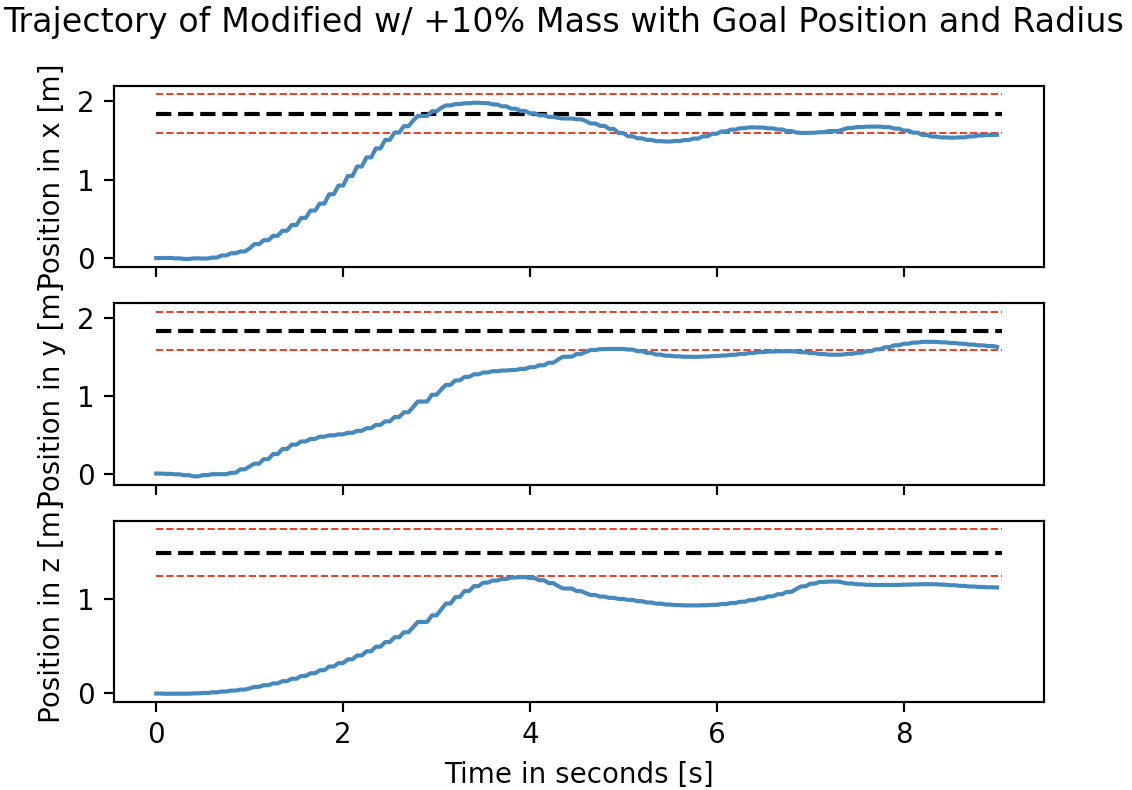
\includegraphics[width=\textwidth]{figures/5_/Testing/ddpg_test_robust+10-2.png}
         \caption{The trajectory of the quadrotor with +10\% mass, compared to the goal position, under guidance of the Modified model.}
         \label{fig:ddpg_test_robust+10-2}
     \end{subfigure} 
     \hfill 
     \begin{subfigure}[b]{0.49\textwidth}
         \centering
         \captionsetup{justification=centering}
         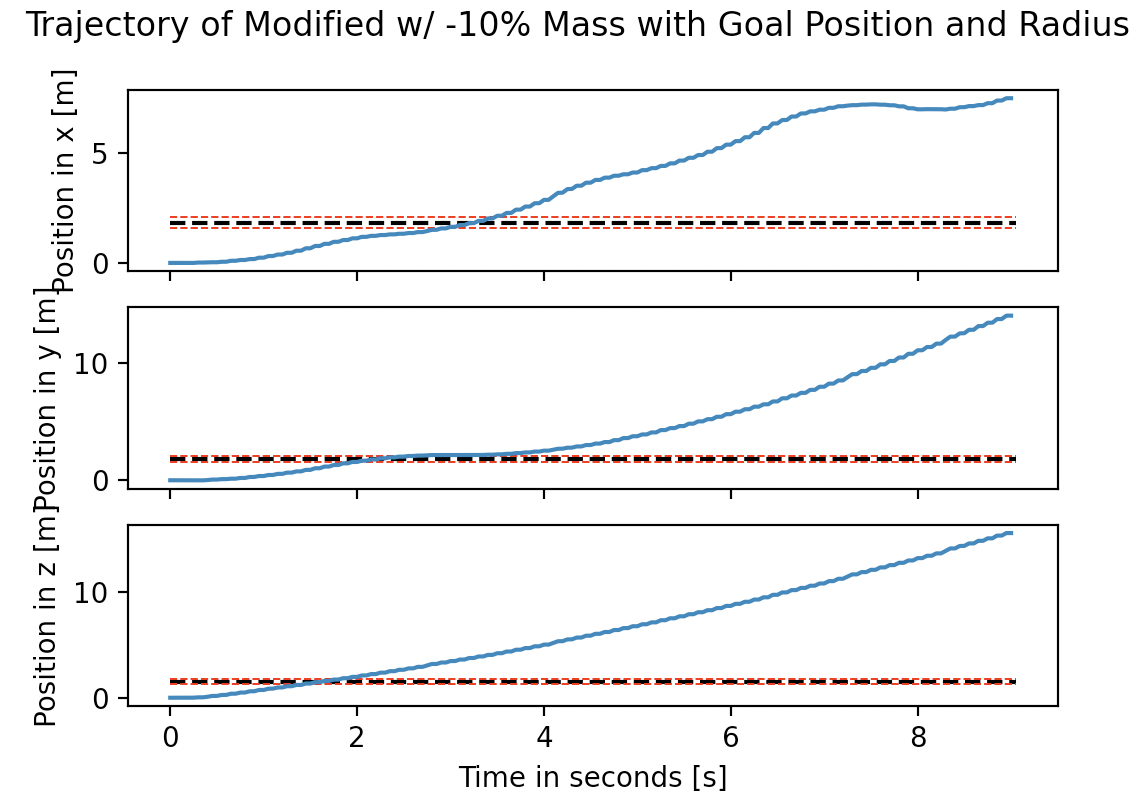
\includegraphics[width=\textwidth]{figures/5_/Testing/ddpg_test_robust-10-2.png}
         \caption{The trajectory of the quadrotor with -10\% mass, compared to the goal position, under guidance of the Modified model.}
         \label{fig:ddpg_test_robust-10-2}
     \end{subfigure} 
    \captionsetup{justification=centering}
    \caption{Test run no. 100 for the Modified and Original DDPG models.}
     \label{fig:ddpg_test_robust}
\end{figure}
From these results, we see that the performance of our DDPG models fall dramatically, with only the Modified model seldom being able to reach the goal in the +10\% mass case. We can also see that the performances in the -10\% mass case is severely impacted, compared to the +10\% case. To see why, we can take a look at Figure \ref{fig:ddpg_test_robust}.
From this figure, we observe two very contrasting behaviours. In the +10\% mass case, the quadrotor does decently to stay on track, settling quite nicely along $x$ and $y$ but struggles to match the goal position along the $z$-axis. In the -10\% mass case, the quadrotor overshoots the goal position by a large margin, basically flying off into the distance and unable to stop. From this, we see that the values in Table \ref{table:5_DDPG_robustnesstests} make sense.
Some considerations and possible explanations for why this happens will be made in Section \ref{sec:6_behaviour_robustnessTest_pm10}.


\section{PPO}
\label{sec:5_PPO}

As mentioned in Section \ref{sec:4_Experiment}, we majority of results are focused around PPO. The list of models are presented in Table \ref{table:5_PPO_hyperparameters}.
\begin{table}[hbt]
    \centering
    \resizebox{\textwidth}{!}{%
    \begin{tabular}{||M{0.7cm}|M{1.6cm}||M{1.8cm}|M{1.8cm}|M{1.7cm}|M{1.4cm}|M{1.4cm}|M{1.4cm}||}
    \hline
    ID & Model & Trajectory, T & Learning rate $\alpha$ & N. opt. epochs, K & N. minibatches & Ent. coef. $c_2$ & VF coef. $c_1$ \\ \hline\hline
    1  & 4-44$\alpha$ & 4000  & 2e-04 & 4  & 4 & 0    & 0.5 \\ \hline
    2  & 4-44       & 4000  & 3e-04 & 4  & 4 & 0    & 0.5 \\ \hline
    3  & 4-44E      & 4000  & 3e-04 & 4  & 4 & 0.01 & 0.5 \\ \hline
    4  & 4-84EV     & 4000  & 3e-04 & 8  & 4 & 0.01 & 1   \\ \hline
    5  & 8-44       & 8000  & 3e-04 & 4  & 4 & 0    & 0.5 \\ \hline
    6  & 8-84EV     & 8000  & 3e-04 & 8  & 4 & 0.01 & 1   \\ \hline
    7  & 8-88EV     & 8000  & 3e-04 & 8  & 8 & 0.01 & 1   \\ \hline
    8 & 8-154       & 8000  & 3e-04 & 15 & 4 & 0    & 0.5 \\ \hline
    9 & 8-154E      & 8000  & 3e-04 & 15 & 4 & 0.01 & 0.5 \\ \hline
    10 & 8-154EV    & 8000  & 3e-04 & 15 & 4 & 0.01 & 1   \\ \hline
    11 & 8-158EV    & 8000  & 3e-04 & 15 & 8 & 0.01 & 1   \\ \hline
    12 & 16-154     & 16000 & 3e-04 & 15 & 4 & 0    & 0.5 \\ \hline
    \end{tabular}%
    }
    \caption{The different PPO models tested, along with their hyperparameters.}
    \label{table:5_PPO_hyperparameters}
\end{table}
The model names here simply refer to its hyperparameters, where for example model 4, ``4-84EV'', has a batch size of 4000, makes 8 optimisations per trajectory, consist of 4 minibatches per trajectory, has an entropy coefficient of 0.01, and value function coefficient of 1.0. If a model does not contain E or V, the entropy and value function coefficients have the values of 0 and 0.5, as in the original implementation in \cite{baselines}. Also, the clipping term $\epsilon$ was chosen to be 0.1.

The choice of models in Table \ref{table:5_PPO_hyperparameters} was made so to be able to make a comparison between hyperparameters. These hyperparameters are initially inspired from the appendix in \cite{PPO}, with some modifications. There are quite a few combinations that did not make the list as over 80 models were tested for this project, with many of them experimental. Though, as a discussion, two of them will be briefly introduced in Section \ref{subsec:6_possible_improvements}.

Furthermore, every model tested here is trained from the same initialisation point to illustrate the effects of each hyperparameter more clearly. This was also decided because we managed to obtain a particularly impressive result from this initialisation point, which we wished to recreate.
Specifically, the initialisation point was a model 4-44 trained for 125 epochs, and the the impressive result was also a 4-44, which we will only look at at the end of this section.

\subsection{Training}
Training the models are done according to the description in Section \ref{sec:4_5_experimentalSetup}. The PPO models required significantly less time to train than its DDPG counterpart, though to reach questionable levels of performance. The epochs of best performance are varying for each of the models, handpicked from the training curves which we will see later.
The time taken to train each of the models to their peak are shown in Table \ref{table:5_PPO_trainingTime}. Note that every model is trained on top of a 4-44 model, trained to 125 epochs, which took 2 hours and 32 minutes.
\begin{table}[hbt]
    \centering
    \begin{tabular}{||M{1cm}|M{2cm}||M{2cm}|M{3cm}|M{3cm}||}
    \hline
    ID & Model & Peak Epoch & Training Time to Peak & Total Time \\ \hline\hline
    1  & 4-44$\alpha$ & 74 &   1h 25m &  3h 57m  \\\hline
    2  & 4-44       &   222 &  4h 16m &  6h 48m\\\hline
    3  & 4-44E      &   200 &  3h 51m &  6h 23m\\\hline
    4  & 4-84EV     &   114 &  2h 14m &  4h 46m\\\hline
    5  & 8-44       &   94 &   3h 36m &  6h 8m\\\hline
    6  & 8-84EV     &   155 &  6h 4m  &  8h 36m\\\hline
    7  & 8-88EV     &   131 &  5h 9m  &  7h 41m\\\hline
    8 & 8-154       &   104 &  3h 59m &  6h 31m\\\hline
    9 & 8-154E      &   110 &  4h 13m &  6h 45m\\\hline
    10 & 8-154EV    &   104 &  4m 1m  &  6m 33m\\\hline
    11 & 8-158EV    &   88 &   3h 26m &  5h 58m\\\hline
    12 & 16-154     &   113 &  8h 40m &  11h 12m\\\hline
    \end{tabular}
    \caption{The time used to train each of the PPO models presented. Since each model is initialised with a pre-trained 4-44 model, the total time compensates for the 2h 32m (125 epochs).}
     \label{table:5_PPO_trainingTime}
\end{table}
From the training times, we see quite a difference compared with the DDPG training times in Table \ref{table:5_PPO_trainingTime}, with the average training time being a third of that of DDPG.

When analysing the results for the training curves, we split the batch of models and only look at models relevant for each hyperparameter. Further, since the training plots are quite small and noisy, every data point is a smoothed with an exponential moving average with weight 0.9. We will also quickly see that the plots look very different compared to the ones for DDPG, though we will also come back to this later in the discussion. For now, the focus will be on the effect of the hyperparameters and the relative performance between the PPO models.

\subsubsection{Understanding The Actor-Critic Losses}
The actor and critic losses corresponds to the \textit{negative} clipped actor objective function $J_t^{CLIP}$ (in \cite{baselines}) and the MSE of the value function estimate and its bootstrapped target value -- the next-state reward and value estimate -- known as the prediction error $\overline{VE}$. These terms are found in Equation \eqref{3_5_objectiveFull}. 
Thus, the critic loss can be associated with PPO's ability to judge the value of its current state, similarly to in DDPG, where a high critic loss correlates to big discrepancies between value estimates in consecutive states, and a \textit{low critic loss} means that the value estimates in consecutive states are similar -- which happens if they are \textit{accurate}.

The actor objective function, $J_t^{CLIP}$, is positive if the advantage $\hat{A}_t$ is positive, which happens if the agent performs better than anticipated. The actor loss (the negative of  $J_t^{CLIP}$) is therefore negative if the agent performs better than anticipated and positive if the actor does worse than expected ($\hat{A}_t$ < 0). As for its magnitude, since $r_t(\bt)$ is clipped, the magnitude of the actor loss thus gives an estimate of how good or bad the actor did compared to its estimate, where then a \textit{large} positive actor loss means \textit{a lot} worse than expected. This follows from Equation \eqref{3_5_clippedObjective}, where $J_t^{CLIP}$ is proportional to $\hat{A}_t$, with $r_t(\theta) \in [1-\epsilon,\, 1+\epsilon]$ and $\epsilon = 0.1$. 


\subsubsection{Trajectory size}
So with interpretation of the plots clear, we can get underway with the results. The first hyperparameter to analyse is the length of the trajectory, $T$. For this, we compare models 4-44, 8-44, 8-154 and 16-154. 
\begin{figure}[hbt]
     \centering
     \begin{subfigure}[b]{0.32\textwidth}
         \centering
         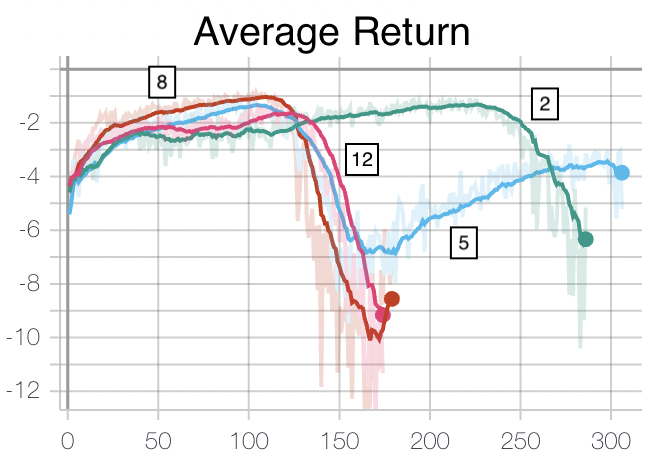
\includegraphics[width=\textwidth]{figures/5_/Training/ppo_trajectory_avgReturn.png}
         \caption{}
         \label{fig:5_training_ppo_trajectoryAvgReturn}
     \end{subfigure} 
     \hfill
     \begin{subfigure}[b]{0.32\textwidth}
         \centering
         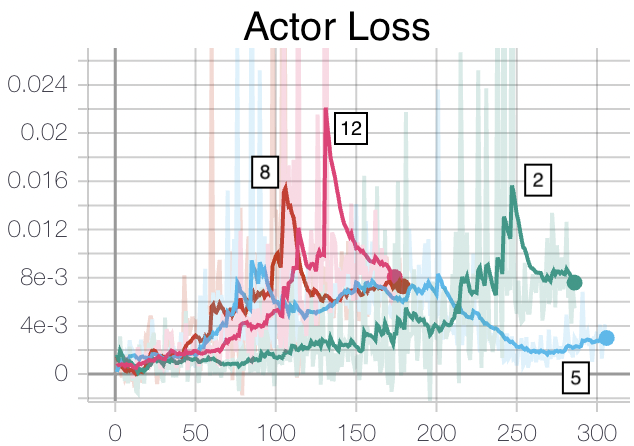
\includegraphics[width=\textwidth]{figures/5_/Training/ppo_trajectory_actorLoss.png}
         \caption{}
         \label{fig:5_training_ppo_trajectoryActorL}
     \end{subfigure}
     \hfill
     \begin{subfigure}[b]{0.32\textwidth}
         \centering
         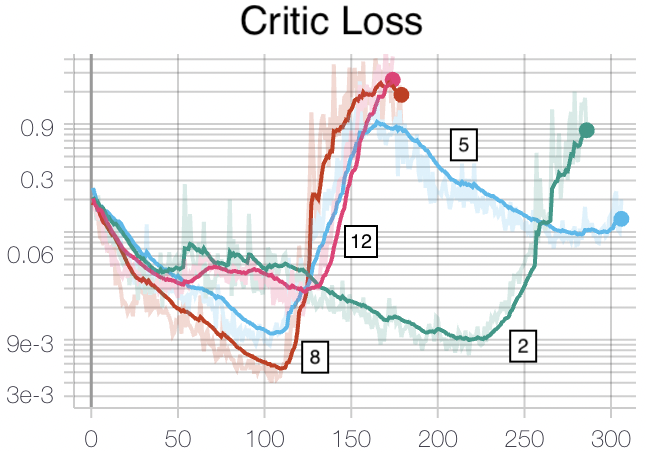
\includegraphics[width=\textwidth]{figures/5_/Training/ppo_trajectory_criticLoss.png}
         \caption{}
         \label{fig:5_training_ppo_trajectoryCriticL}
     \end{subfigure}
    \captionsetup{justification=centering}
    \caption{The effect of changing the length of the trajectory, $T$. There are two comparisons made, one between models 2: 4-44 and 5: 8-44, and the other between 8: 8-154 and 12: 16-154.}
     \label{fig:5_training_ppo_trajectory}
\end{figure}
From \cref{fig:5_training_ppo_trajectoryAvgReturn}, the effect of the trajectory length is varying. For models 2 and 5, we see that increasing the batch size from 4000 to 8000 does leads to faster training in terms of number of epochs, with both models reaching roughly the same average return at epochs 222 and 94. However, the ``speed'' is actually quite misleading, since one epoch requires double the number of experiences, such that the training times are also roughly the same. This can be confirmed through the training times in Table \ref{table:5_PPO_trainingTime} for models 2 and 5. Next, when the number of optimisation epochs are set to 15, we see that increasing the batch size further to 16000 from 8000 reduces performance, both in terms of peak average return, but also time required to train. 

We also see a correlation between the average return and critic loss, such that the agent gets better at predicting its value estimates at the same time it performs better in the environment too. It is unclear if there is some cause-effect at play between the two, but it makes sense that they are correlated since an agent performing well should be good at understanding the values of states and an agent who understands values of states will make good decisions.

For the actor loss, we can first observe that they are all positive. This means that the agent consistently finds its actions worse than expected, despite the critic getting better at estimate values of states and the average return increasing. Further, we also see spikes for each model which then are directly related to the sudden drop in average return. This means that when the average return drops, this is surprising to the agent as well and yields a large negative advantage. As the rate of change of return stabilises, then the actor loss reduces. Strangely however, there is a build up of actor loss \textit{before} each peak, which suggests that the agent thinks that is its performing increasingly worse than expected, despite that we can clearly see the average return increasing. This will be further explored in Section \ref{sec:6_underperformance_divergence_PPO}.

\subsubsection{Learning rate}
The next hyperparameter of interest is the learning rate, which has strong ties theoretical ties to the length of the trajectory (batch size) \cite{batchsizeInvariance,dontdecayLRIncreaseBatch,ImageNet1Hour}. The models compared are 4-44$\alpha$ and 4-44. 
\begin{figure}[hbt]
     \centering
     \begin{subfigure}[b]{0.32\textwidth}
         \centering
         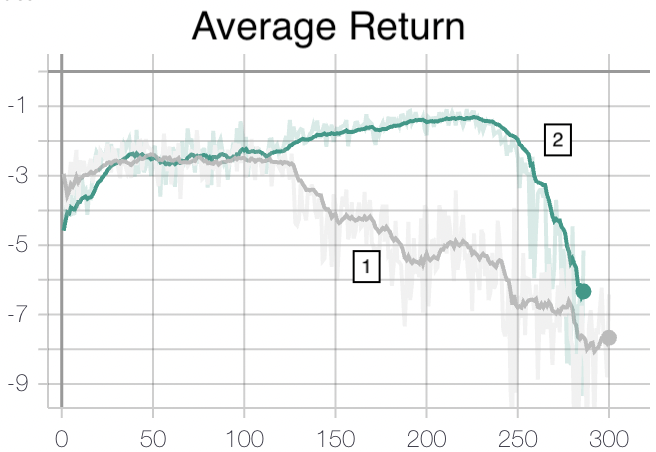
\includegraphics[width=\textwidth]{figures/5_/Training/ppo_learningRateAvgReturn.png}
         \caption{}
         \label{fig:5_training_ppo_learningRateAvgReturn}
     \end{subfigure} 
     \hfill
     \begin{subfigure}[b]{0.32\textwidth}
         \centering
         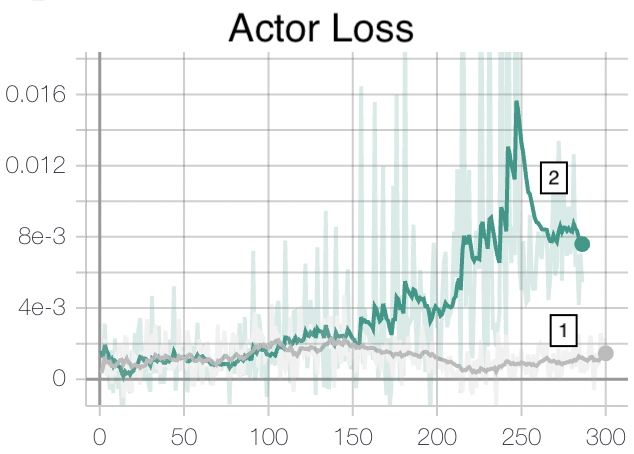
\includegraphics[width=\textwidth]{figures/5_/Training/ppo_learningRateActorL.png}
         \caption{}
         \label{fig:5_training_ppo_learningRateActorL}
     \end{subfigure}
     \hfill
     \begin{subfigure}[b]{0.32\textwidth}
         \centering
         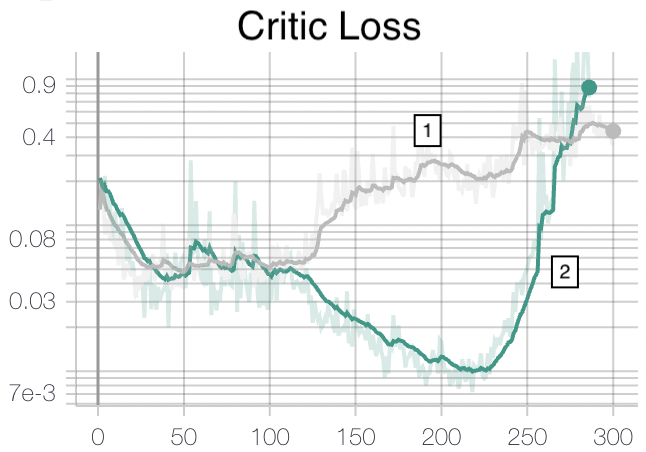
\includegraphics[width=\textwidth]{figures/5_/Training/ppo_learningRateCriticL.png}
         \caption{}
         \label{fig:5_training_ppo_learningRateCriticL}
     \end{subfigure}
    \captionsetup{justification=centering}
    \caption{The effect of changing the learning rate $\alpha$, seen through the comparison of models 1: 4-44$\alpha$ and 2: 4-44.}
     \label{fig:5_training_ppo_learningRate}
\end{figure}
From Figure \ref{fig:5_training_ppo_learningRate}, we see that reducing the learning rate from 3e-4 to 2e-4 leads to a lower performance on average, with no clear indication that model \one will improve beyond model 4-44, apart for when \two diverges. Interestingly, the actor loss is quite low with very minimal variance in consecutive epochs. This means that the agent does perform ``as expected'', though what this expectation is is a bit unclear given the high critic loss. This result is an example that reducing the learning rate in our implementation was not beneficial to performance, and so is the only comparison shown.


\subsubsection{Entropy Coefficient}
The entropy coefficient, in theory, should be related to the degree of exploration in seen in the agent. For on-policy methods, this is well-received and we hope to see the agents finding a better behaviour than in the previous plots. For this hyperparameter, we will comparing models, 4-44, 4-44E, 8-154 and 8-154E.
\begin{figure}[hbt]
     \centering
     \begin{subfigure}[b]{0.32\textwidth}
         \centering
         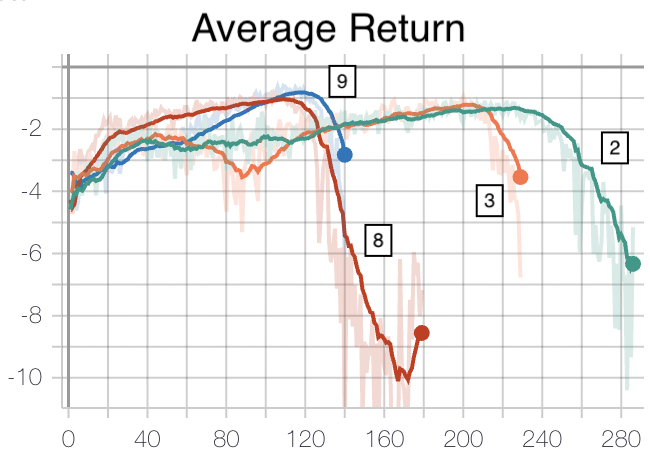
\includegraphics[width=\textwidth]{figures/5_/Training/ppo_entcoefAvgReturn.png}
         \caption{}
         \label{fig:5_training_ppo_entcoefAvgReturn}
     \end{subfigure} 
     \hfill
     \begin{subfigure}[b]{0.32\textwidth}
         \centering
         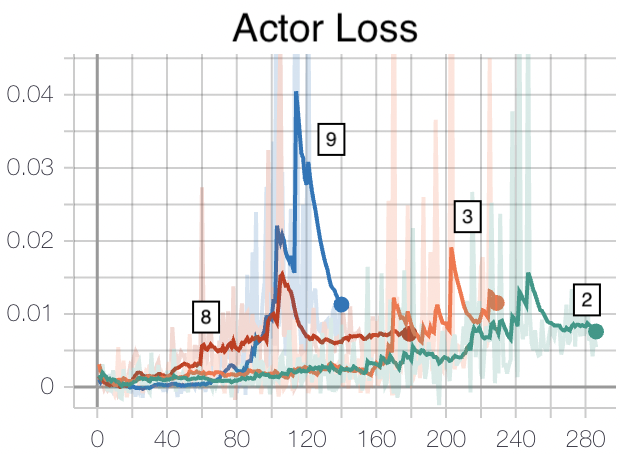
\includegraphics[width=\textwidth]{figures/5_/Training/ppo_entcoefActorL.png}
         \caption{}
         \label{fig:5_training_ppo_entcoefActorL}
     \end{subfigure}
     \hfill
     \begin{subfigure}[b]{0.32\textwidth}
         \centering
         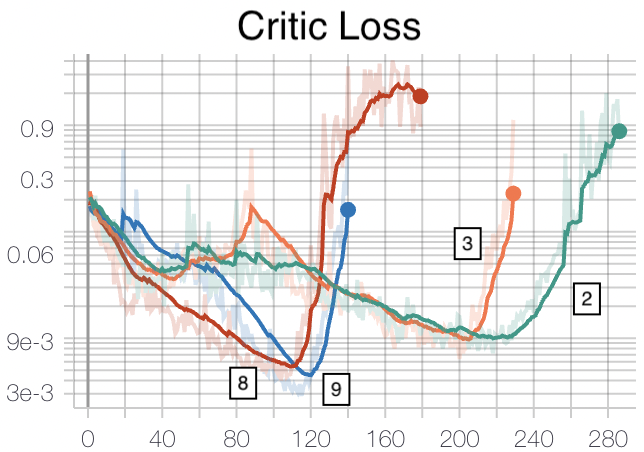
\includegraphics[width=\textwidth]{figures/5_/Training/ppo_entcoefCriticL.png}
         \caption{}
         \label{fig:5_training_ppo_entcoefCriticL}
     \end{subfigure}
    \captionsetup{justification=centering}
    \caption{The effect of changing the entropy term coefficient, $c_2$. There are two comparisons made, between models 2: 4-44 and 3: 4-44E, and between 8: 8-154 and 9: 8-154E.}
     \label{fig:5_training_ppo_entcoef}
\end{figure}
From \cref{fig:5_training_ppo_entcoef}, we observe varying results. Adding entropy loss does not have a significant effect for the 4-44E model, but leads to a marginally better peak average return, seen in the 8-154E model. Without high expectations, this was a good indication that the entropy term was beneficial.

Another interesting result is that the actor losses for the entropy models peak higher than their no-entropy counterparts. Since the entropy loss term is independent of the clipped actor objective, and the average returns and critic losses are also quite similar, the reason for why this is is unclear.


\subsubsection{Value function Coefficient}
In this project, we increased the value function coefficient from 0.5 to 1.0. This does not directly change the value function loss, but determines its weight in the total loss. As a result, we should achieve larger updates to the critic with a higher coefficient. To see what happens, we will compare the models 8-154E and 8-154EV.
\begin{figure}[hbt]
     \centering
     \begin{subfigure}[b]{0.32\textwidth}
         \centering
         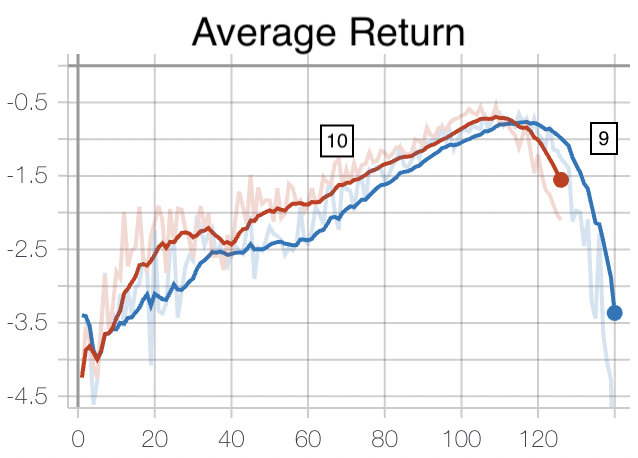
\includegraphics[width=\textwidth]{figures/5_/Training/ppo_vfcoeffAvgReturn.png}
         \caption{}
         \label{fig:5_training_ppo_vfcoeffAvgReturn}
     \end{subfigure} 
     \hfill
     \begin{subfigure}[b]{0.32\textwidth}
         \centering
         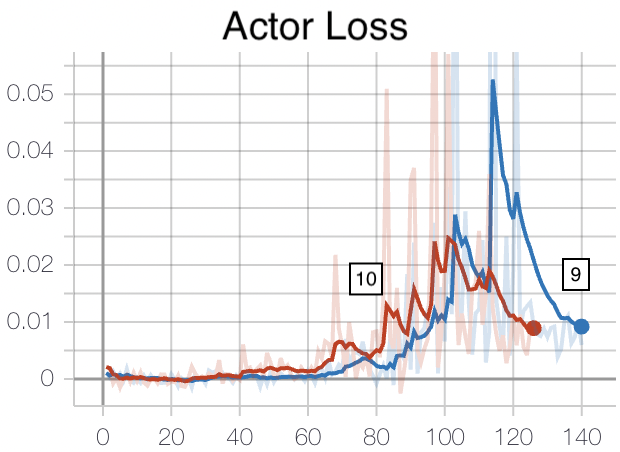
\includegraphics[width=\textwidth]{figures/5_/Training/ppo_vfcoeffActorL.png}
         \caption{}
         \label{fig:5_training_ppo_vfcoeffActorLoss}
     \end{subfigure}
     \hfill
     \begin{subfigure}[b]{0.32\textwidth}
         \centering
         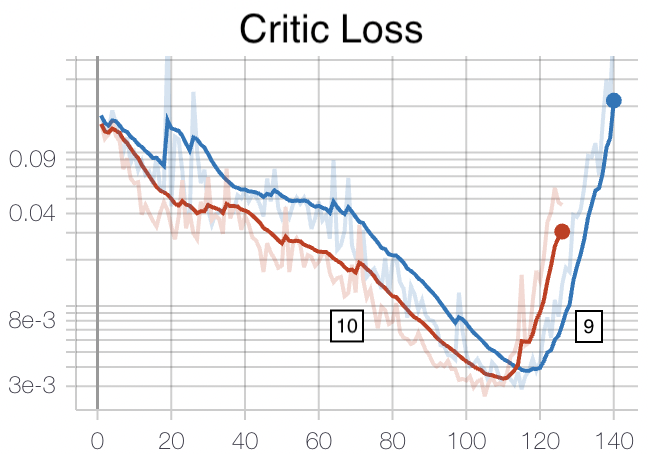
\includegraphics[width=\textwidth]{figures/5_/Training/ppo_vfcoeffCriticL.png}
         \caption{}
         \label{fig:5_training_ppo_vfcoeffCriticLoss}
     \end{subfigure}
    \captionsetup{justification=centering}
    \caption{The effect of changing the value function coefficient, $c_1$. This is a comparison between models 9: 8-154E and 10: 8-154EV.}
     \label{fig:5_training_ppo_vfcoeff}
\end{figure}
Based on Figure \ref{fig:5_training_ppo_vfcoeff}, we see that larger critic updates yields a slightly better performance overall. In \cref{fig:5_training_ppo_vfcoeffCriticLoss}, we observe that the critic loss in model \ten falls quicker than model \nine and matches our initial guess. Further, the relationship between the average return and the critic loss is highlighted clearly here, where our understanding that a low critic loss is beneficial to agent performance is true to a large extent.


\subsubsection{Number of optimisation epochs}
The number of optimisation epochs $K$, denotes the number of times we should update our weights based on the same trajectory. From this intuition, we expect that larger $K$ values should lead to faster learning, which could maybe lead to instability. 
\begin{figure}[hbt]
     \centering
     \begin{subfigure}[b]{0.32\textwidth}
         \centering
         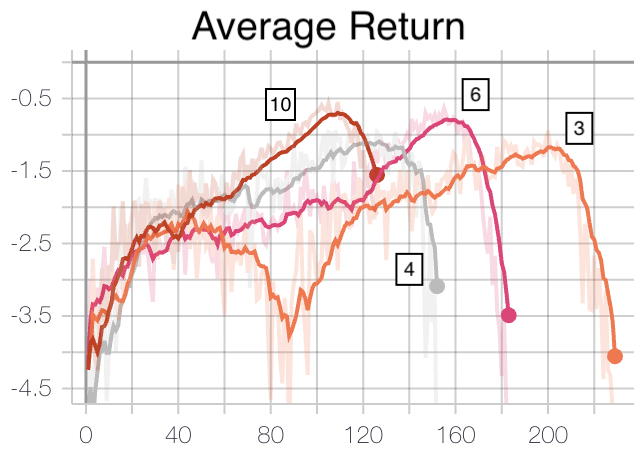
\includegraphics[width=\textwidth]{figures/5_/Training/ppo_noptepochsAvgReturn.png}
         \caption{}
         \label{fig:5_training_ppo_noptepochsAvgReturn}
     \end{subfigure} 
     \hfill
     \begin{subfigure}[b]{0.32\textwidth}
         \centering
         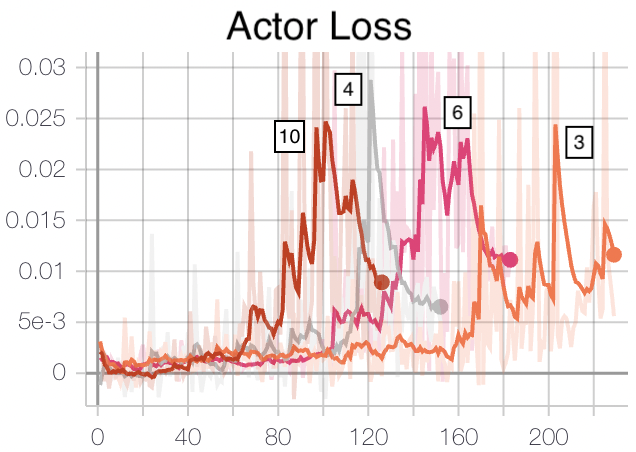
\includegraphics[width=\textwidth]{figures/5_/Training/ppo_noptepochsActorL.png}
         \caption{}
         \label{fig:5_training_ppo_noptepochsActorL}
     \end{subfigure}
     \hfill
     \begin{subfigure}[b]{0.32\textwidth}
         \centering
         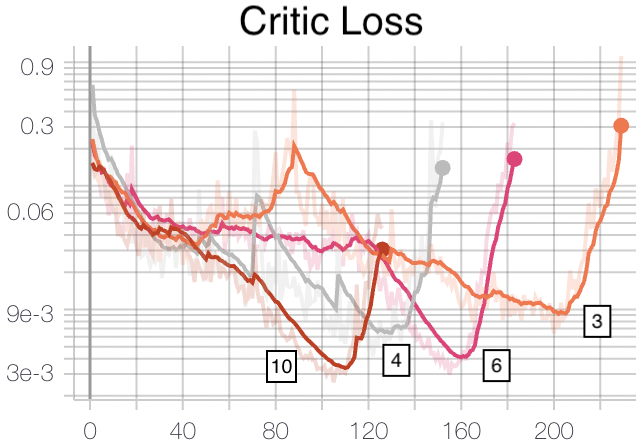
\includegraphics[width=\textwidth]{figures/5_/Training/ppo_noptepochsCriticL.png}
         \caption{}
         \label{fig:5_training_ppo_CriticL}
     \end{subfigure}
    \captionsetup{justification=centering}
    \caption{The effect of changing the number of optimisation epochs, $K$. Presented are two comparisons, between models 3: 4-44E and 4: 4-84EV, and 6: 8-84EV and 10: 8-154EV}
     \label{fig:5_training_ppo_noptepochs}
\end{figure}
\cref{fig:5_training_ppo_noptepochs} shows four models with similar shape, with models \ten and \six with highest average return, and \three and \four slightly below. From this, we see that there is no significant impact in the peak average return value when changing $K$, but we do observe that the \textit{training times are reduced significantly}. In that sense, our original expectation that instability occurs faster is also true. The actor and critic loss plots are very similar to the ones seen before and we can begin to see a trend in how the training curves are shaped for all models.


\subsubsection{Number of minibatches}
The number of minibatches indirectly controls the minibatch size, which is a hyperparameter often tuned in deep learning. From this, we know that small minibatches produce more noisy gradient updates compared to full-batch gradient updates. For this hyperparameter we will be comparing models 8-84EV, 8-88EV, 8-154EV and 8-158EV.
\begin{figure}[hbt]
     \centering
     \begin{subfigure}[b]{0.32\textwidth}
         \centering
         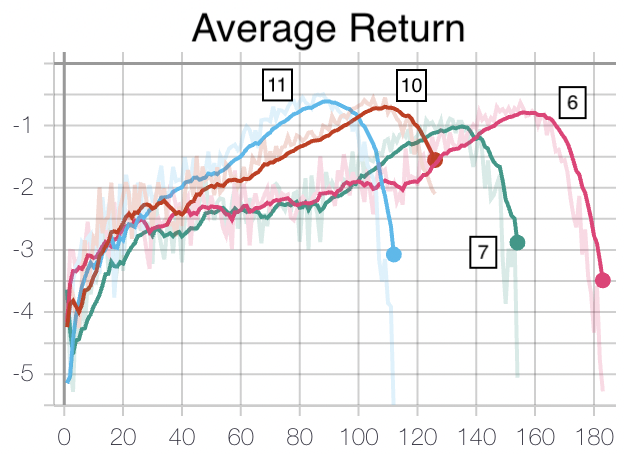
\includegraphics[width=\textwidth]{figures/5_/Training/ppo_nminibatchAvgReturn.png}
         \caption{}
         \label{fig:5_training_ppo_nminibatchAvgReturn}
     \end{subfigure} 
     \hfill
     \begin{subfigure}[b]{0.32\textwidth}
         \centering
         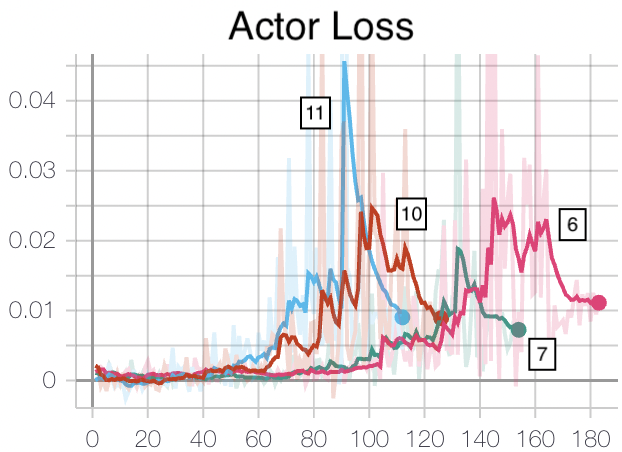
\includegraphics[width=\textwidth]{figures/5_/Training/ppo_nminibatchActorL.png}
         \caption{}
         \label{fig:5_training_ppo_nminibatchActorL}
     \end{subfigure}
     \hfill
     \begin{subfigure}[b]{0.32\textwidth}
         \centering
         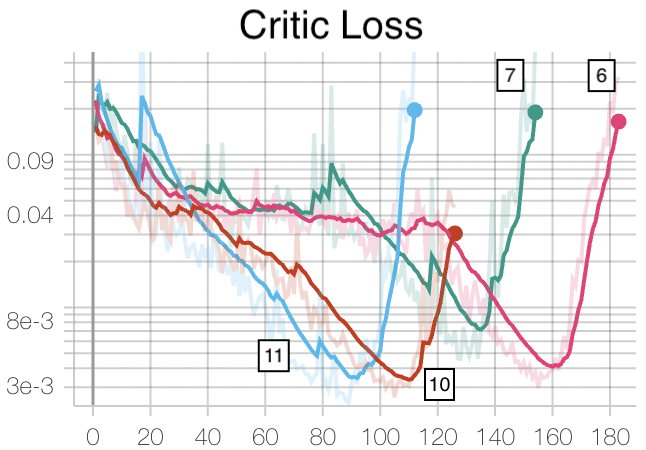
\includegraphics[width=\textwidth]{figures/5_/Training/ppo_nminibatchCriticL.png}
         \caption{}
         \label{fig:5_training_ppo_nminibatchCriticL}
     \end{subfigure}
    \captionsetup{justification=centering}
    \caption{The effect of changing the number of minibatches. There are two comparison for this, in models 6: 8-84EV, 7: 8-88EV, 10: 8-154EV, 11: 8-158EV.}
     \label{fig:5_training_ppo_nminibatch}
\end{figure}
In Figure \ref{fig:5_training_ppo_nminibatch}, we see that the training plots produced are not at all expected, given that the assumed effect of this hyperparameter was just more or less noisy updates. We observe that increasing the number of minibatches produces a similar response as that of the number of optimisation epochs, where the \textit{speed of learning} is significantly impacted. Apart from this, the effect on performance is varying, where doubling the number of minibatches in \seven leads to worse performance compared to 8-84EV, whereas \eleven has a slightly better performance than \ten. 

To explain this, a closer look was taken into the implementation of PPO in \cite{baselines}. From this we realised that the number of minibatches was also directly proportional to the number of gradient updates made. In other words, when the number of minibatches is doubled, so is the number of gradients calculated and applied to the networks, which is a bit obvious in hindsight. 
Based on this reasoning, it makes sense that doubling the number of minibatches results in roughly the same effect as doubling the number of optimisation epochs. 
Yet, exactly what happens is a bit unclear, since we expect the sum of losses per minibatch to be halved when the number of minibatches is doubled, so that despite more gradients applied, each gradient update is smaller. To guess why -- since we also clip the actor-objective -- taking many small gradient updates perhaps makes a larger overall update per epoch, compared to fewer larger updates when the number of minibatches is low, though this is not for certain.


\subsubsection{Best Models and the Optimal Model}
Now that we have seen the effect of different hyperparameters in training we look at some of the best models found. These are the models 8-84EV, 8-154E, 8-154EV and 8-158EV, shown in \cref{fig:5_training_ppo_bestModels}.
\begin{figure}[hbt]
     \centering
     \begin{subfigure}[b]{0.32\textwidth}
         \centering
         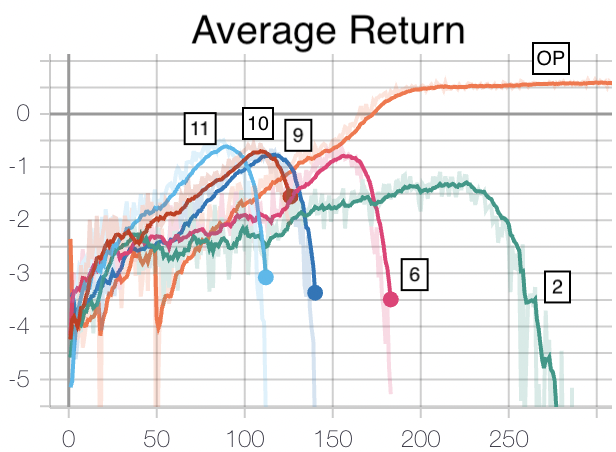
\includegraphics[width=\textwidth]{figures/5_/Training/ppo_bestmodelsAvgReturn.png}
         \caption{}
         \label{fig:5_training_ppo_bestModelsAvgReturn}
     \end{subfigure} 
     \hfill
     \begin{subfigure}[b]{0.32\textwidth}
         \centering
         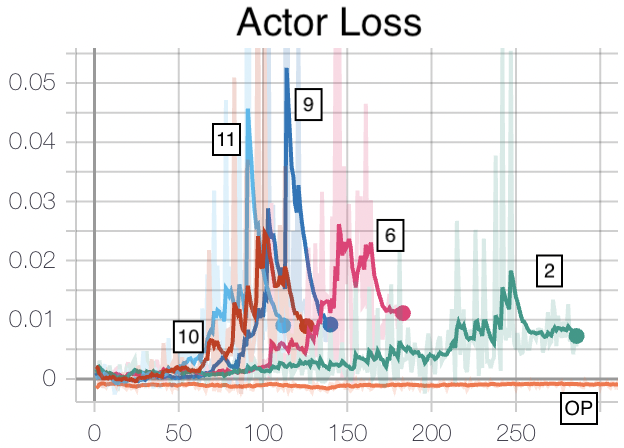
\includegraphics[width=\textwidth]{figures/5_/Training/ppo_bestmodelsActorL.png}
         \caption{}
         \label{fig:5_training_ppo_bestModelsActorL}
     \end{subfigure}
     \hfill
     \begin{subfigure}[b]{0.32\textwidth}
         \centering
         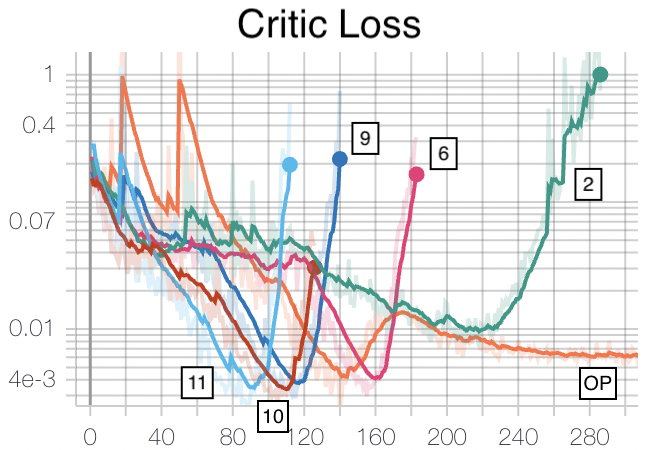
\includegraphics[width=\textwidth]{figures/5_/Training/ppo_bestmodelsCriticL.png}
         \caption{}
         \label{fig:5_training_ppo_bestModelsCriticL}
     \end{subfigure}
    \captionsetup{justification=centering}
    \caption{The training plots for the best models found for PPO. These are 6: 8-84EV, 9: 8-154E, 10: 8-154EV and 11: 8-158EV. Also included is our Optimal model, OP. Model 2: \two is included for reference.}
     \label{fig:5_training_ppo_bestModels}
\end{figure}
From this figure, we observe that the best average returns achieved are roughly the same, in between -0.5 and -0.9.
Looking very closely, there is a marginal difference, with model \eleven best, then 8-154EV, 8-154E, and
8-84EV. This is also the case for the lowest critic losses, though not so apparent in the smoothed \cref{fig:5_training_ppo_bestModelsCriticL}.
Unintuitively, \eleven also tops the ranking for the speed of training and took the shortest time to train to peak. 

We also present our optimally trained model, OP, which is of the same type as model 2 in \cref{fig:5_training_ppo_bestModels}, a 4-44. However, we see two very different training plots, where the OP model converges to an Optimal result with an average return of about 0.5, while Model 2 diverges.
We note that the OP model follows a similar training pattern as the other models though, with consistent improvement (seen until epoch 140) and a characteristic ``dip'' in the critic loss. However, as the other models then diverge after this dip, we see that the OP model instead is able to recover -- finding a ``good gradient descent path'' in the critic ``solution space'', and manages to keep improving its performance. This suggests that the ``dip'' in the critic loss and its corresponding peak in the average return could be understood as a \textit{local optimum} in the solution space that is simple to reach, while the \textit{global optimum} gradient descent path is much more difficult to find.

Another observation is that the actor loss for the OP model is always negative. This means that the agent always performed better than it expected, throughout its whole training period. This is very unique, since by pure randomness we would expect that at least at one point of its training should the agent do worse than it expected.


\subsubsection{Brief Summary}

All in all, we have seen that having a batch size of 8000 is beneficial to training in general, along with entropy and a higher value function coefficient. We observed that adding entropy loss for exploration was advantageous and slightly improved the peak average return, while the value function coefficient was a boost to reducing the critic loss, in turn improving training speed and slightly increased the peak average return.

To pair with this, one can choose to increase the number of optimisation epochs to either 8 or 15, while keeping the number of minibatches at 4 or increased to 8. These should then improve the training speed but not affect the peak average return attained.

Despite all our training efforts, the Optimal model does not follow this general guideline, but still managed to outperform all other models with a relatively simpler hyperparameter combination. This serves to remind us that hyperparameter tuning can only do so much in deep reinforcement leaning and the best models can be found unexpectedly with a bit of luck.


\subsection{Testing}
Now that we have seen the training results of our models we can begin to compare their performances in a standardised format to see if their training reflects their performance. In the Best Models section, it was briefly mentioned that the peaks in average returns for our models were possibly local optima. Thus, it will also be interesting to see what kind of behaviour this entails.

The test results are compiled into Table \ref{table:5_PPO_allTests}.
\begin{table}[hbt]
    \centering
    \begin{tabular}{||M{0.7cm}|M{1.6cm}||M{2.5cm}|M{2.5cm}|M{2.5cm}||}
    \hline
    ID & Model  & Goal rate & Average Return & Average RMSE   \\\hline\hline
    1	& 4-44$\alpha$ & 0 & -3.1027 &	0.1377 \\\hline
    2	& 4-44         & 0 & -2.3178 &	0.1000 \\\hline
    3	& 4-44E        & 0 & -2.1601 &	0.0767 \\\hline
    4	& 4-84EV       & 0 & -3.5790 &	0.0805 \\\hline
    5	& 8-44         & 0 & -1.9443 &	0.0528 \\\hline
    6	& 8-84EV       & 0 & -1.0316 &	0.0364 \\\hline
    7	& 8-88EV       & 0 & -2.5957 &	0.0685 \\\hline
    8	& 8-154        & 0 & -6.1768 &	0.1115 \\\hline
    9	& 8-154E       & 2 & -1.7125 &	0.0696 \\\hline
    10	& 8-154EV      & 3 & -3.0630 &	0.0660 \\\hline
    11	& 8-158EV      & 79 & -4.0786 &	0.0731 \\\hline
    12	& 16-154       & 0 & -2.6880 &	0.0693 \\\hline\hline
    OP & Optimal (4-44) & 100 &	0.4294 & 0.0181 \\\hline
    \end{tabular}
    \caption{The test results for all the PPO models. Each model was run 100 times on a constant waypoint task. Then, the goal rate, average return and average RMSE to the shortest path was recorded.}
     \label{table:5_PPO_allTests}
\end{table}
To do an analysis of how the different hyperparameters correlate to performance in tests, we will break down \cref{table:5_PPO_allTests} similarly to how the training results were presented.

\subsubsection{Trajectory size}
\begin{table}[hbt]
    \centering
    \begin{tabular}{||M{0.7cm}|M{1.6cm}||M{2.5cm}|M{2.5cm}|M{2.5cm}||}
    \hline
ID & Model  & Goal rate & Average Return & Average RMSE   \\\hline\hline
2  & 4-44   & 0 & -2.3178 & 0.1000 \\\hline
5  & 8-44   & 0 & -1.9443 & 0.0528 \\\hline
8  & 8-154  & 0 & -6.1768 & 0.1115 \\\hline
12 & 16-154 & 0 & -2.6880 & 0.0693
     \\\hline
    \end{tabular}
    \caption{The relevant PPO test results for comparing the length of the trajectory, $T$.}
    \label{table:5_PPO_test_trajectory}
\end{table}
For the length of the trajectory, it was found that there was no significant difference when training models 4-44 and 8-44, while model 8-154 was better than 16-154.
Looking at \cref{table:5_PPO_test_trajectory}, we see that there is a significant difference in test performances compared to training. First, we see that the average return and RMSE for model \five was better than 4-44, with model \five having almost half the RMSE on average.
Next, we see that \eight is much worse than 16-154. This is unexpected since the extent of the difference is very significant. Doing a check into the results for model 8-154, it was found that there were only four runs with a return less -6.18, but with an average return of less than $-63$. By removing these the average increases to -1.72, which explains a lot, but leads to another question of why these anomalies occur. Removing the 7 runs above the mean return for \five leads to an average of -1.75. Thus, its average return in \cref{table:5_PPO_test_trajectory} is very representative of the true return. This is also the case for model 4-44, with only one anomaly run (less than -2.45) with a return of -18.45, which leads to an adjusted average return of -2.15.


\subsubsection{Learning rate}
\begin{table}[hbt]
    \centering
    \begin{tabular}{||M{0.7cm}|M{1.6cm}||M{2.5cm}|M{2.5cm}|M{2.5cm}||}
    \hline
ID & Model  & Goal rate & Average Return & Average RMSE   \\\hline\hline
    1&	4-$\alpha$&	0&	-3.1027	&0.1377 \\\hline
    2&	4-44&	0&	-2.3178	&0.1000 \\\hline
    \end{tabular}
    \caption{The relevant PPO test results for comparing the learning rate, $\alpha$.}
    \label{table:5_PPO_test_learningRate}
\end{table}
Moving on the learning rate, we expect that model \two is
better 4-44$\alpha$.
From \cref{table:5_PPO_test_learningRate} we see that this expectation holds true, with model 4-44 having both a higher average return and lower RMSE than 4-44$\alpha$.

\subsubsection{Entropy Coefficient}
\begin{table}[hbt]
    \centering
    \begin{tabular}{||M{0.7cm}|M{1.6cm}||M{2.5cm}|M{2.5cm}|M{2.5cm}||}
    \hline
ID & Model  & Goal rate & Average Return & Average RMSE   \\\hline\hline
2 & 4-44   & 0 & -2.3178 & 0.1000 \\\hline
3 & 4-44E  & 0 & -2.1601 & 0.0767 \\\hline
8 & 8-154  & 0 & -6.1768 & 0.1115 \\\hline
9 & 8-154E & 2 & -1.7125 & 0.0696
     \\\hline
    \end{tabular}
    \caption{The relevant PPO test results for comparing the effect of the entropy coefficient, $c_2$.}
    \label{table:5_PPO_test_ent_coef}
\end{table}
As for the entropy coefficient, our expectation that entropy yields slightly better performances are also true, seen from \cref{table:5_PPO_test_ent_coef}.
This also includes the fact that the adjusted average return for model \eight is at roughly 1.72, while the average return for 8-154E is already lower than this, without adjustment.


\subsubsection{Value Function Coefficient}
\begin{table}[hbt]
    \centering
    \begin{tabular}{||M{0.7cm}|M{1.6cm}||M{2.5cm}|M{2.5cm}|M{2.5cm}||}
    \hline
ID & Model  & Goal rate & Average Return & Average RMSE   \\\hline\hline
9  & 8-154E  & 2 & -1.7125 & 0.0696 \\ \hline
10 & 8-154EV & 3 & -3.0630 & 0.0660
     \\\hline
    \end{tabular}
    \caption{The relevant PPO test results for comparing the effect of the value function coefficient, $c_1$.}
    \label{table:5_PPO_test_vf_coef}
\end{table}
For the value function coefficient, the average returns are not as expected, with model \ten having a lower return than 8-154E. However, we see that this is not true when considering both the goal rate and the average RMSE. Thus, a usual suspicion that there are anomalies in the test runs for \ten pulling its average down. Compensating for 11 runs with return less than -3, model \ten then has an average of -1.09. When removing the 21 runs with return less than -1.71 for 8-154E, the average return increases to -1.25. This discovery is then a strong result for the value function coefficient.

\subsubsection{Number of optimisation epochs}
\begin{table}[hbt]
    \centering
    \begin{tabular}{||M{0.7cm}|M{1.6cm}||M{2.5cm}|M{2.5cm}|M{2.5cm}||}
    \hline
ID & Model  & Goal rate & Average Return & Average RMSE   \\\hline\hline
3 & 4-44E  & 0 & -2.1601 & 0.0767 \\\hline
4  & 4-84EV  & 0 & -3.5790 & 0.0805 \\\hline
6  & 8-84EV  & 0 & -1.0316 & 0.0364 \\\hline
10 & 8-154EV & 3 & -3.0630 & 0.0660
     \\\hline
    \end{tabular}
    \caption{The relevant PPO test results for comparing the number of optimisation epochs, $K$.}
    \label{table:5_PPO_test_noptepochs}
\end{table}
In \cref{table:5_PPO_test_noptepochs}, we observe that the increasing the number of optimisation epochs results in significantly poorer performances overall. This does not fit our results from training, which suggests that the number of optimisation epochs should not affect performance in general, rather just the training time. 

However, we observe that while the average return is higher and RMSE lower, model \ten is able to reach the goal state while \six is not. Another consideration is that from the Trajectory comparison, we found that adjusting the returns for models \eight and \five resulted in average returns -1.72 and -1.75, which is in contrast to \cref{table:5_PPO_test_noptepochs}. However, having made the adjustment for model \ten already, we see that model model \six is still better compared to the adjusted values of model 8-154EV, which has an average return of 1.09 and RMSE of 0.04309. Thus, we see that model \six is in fact one of our best models.


\subsubsection{Number of minibatches}
\begin{table}[hbt]
    \centering
    \begin{tabular}{||M{0.7cm}|M{1.6cm}||M{2.5cm}|M{2.5cm}|M{2.5cm}||}
    \hline
ID & Model  & Goal rate & Average Return & Average RMSE   \\\hline\hline
6  & 8-84EV  & 0  & -1.0316 & 0.0364 \\\hline
7  & 8-88EV  & 0  & -2.5957 & 0.0685 \\\hline
10 & 8-154EV & 3  & -3.0630 & 0.0660 \\\hline
11 & 8-158EV & 79 & -4.0786 & 0.0731
     \\\hline
    \end{tabular}
    \caption{The relevant PPO test results for comparing the number of minibatches.}
    \label{table:5_PPO_test_nminibatches}
\end{table}
Our expectation from training is that number of minibatches should have the same effect as the number of optimisation epochs and therefore not affect performance. From \cref{table:5_PPO_test_nminibatches}, we see that when the number of minibatches is doubled, the average return decreases and the average RMSE increases, yet the likelihood of reaching goal increases.
Thus, the effect of the number of minibatches resembles the effect of the number of optimisation epochs in \cref{table:5_PPO_test_noptepochs} to a great extent.

To be sure, the results of \eleven were adjusted by removing its 8 below-average runs. This yielded a much higher average return of -0.1332 and RMSE of 0.0440. This result reflects the goal rate much better, but still does not explain why it has such significant anomaly runs. 
Nonetheless, we can still consider \eleven one of our best models.

\subsubsection{Best Models and the Optimal Model}
\begin{table}[hbt]
    \centering
    \resizebox{\textwidth}{!}{
    \begin{tabular}{||M{0.7cm}|M{1.8cm}||M{1.5cm}|M{2.5cm}|M{2cm}||M{2.5cm}|M{2.5cm}|M{1.5cm}||}
    \hline
ID & Model  & Goal rate & Average Return & Average RMSE & Avg. Return w/o outliers & Avg. RMSE w/o outliers & Num. outliers   \\\hline\hline
6  & 8-84EV  & 0   & -1.0316 & 0.0364 & -1.0316 & 0.0364 & 0 \\\hline
9  & 8-154E  & 2   & -1.7125 & 0.0696 & -1.4446 & 0.0657 & 1 \\\hline
10 & 8-154EV & 3   & -3.0630 & 0.0660 & -1.1990 & 0.0457 & 8 \\\hline
11 & 8-158EV & 79  & -4.0786 & 0.0731 & -0.1332 & 0.0440 & 8 \\\hline\hline
OP & Optimal (4-44) & 100 & 0.4294 & 0.0181 & 0.4294 & 0.0181 & 0
     \\\hline
    \end{tabular}}
    \caption{The best models and best hyperparameter combinations found for PPO. These are compared against our Optimal model, OP. Results that ignore episodes with an average return of less than -5 are also shown.}
    \label{table:5_PPO_test_bestModels}
\end{table}
The best models found for PPO are summarised in \cref{table:5_PPO_test_bestModels}.
We can start by observing that model 8-84EV is by far the most consistent model, achieving the highest average return and lowest RMSE, even after adjusting the results for the other models. In contrast, model \eleven is the most inconsistent model, having the most extreme outliers which negatively affects its otherwise good result.

Next, we observe that our Optimal model has a 100\% goal rate, achieving an average reward that reflects its training results very well.

\begin{figure}[H]
     \centering
     \begin{subfigure}[b]{0.48\textwidth}
         \centering
         \captionsetup{justification=centering}
         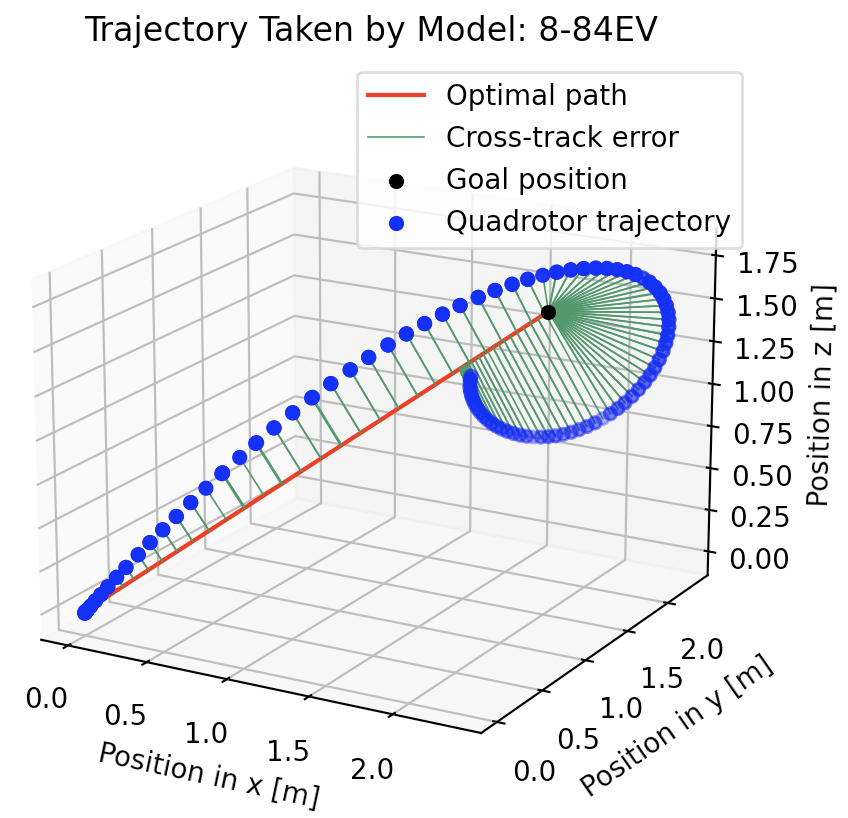
\includegraphics[width=\textwidth]{figures/5_/Testing/ppo_test_884EV1.png}
         \caption{Trajectory of 8-84EV.}
         \label{fig:testing_ppo884EV1}
     \end{subfigure} 
     \hfill 
    \begin{subfigure}[b]{0.49\textwidth}
         \centering
         \captionsetup{justification=centering}
         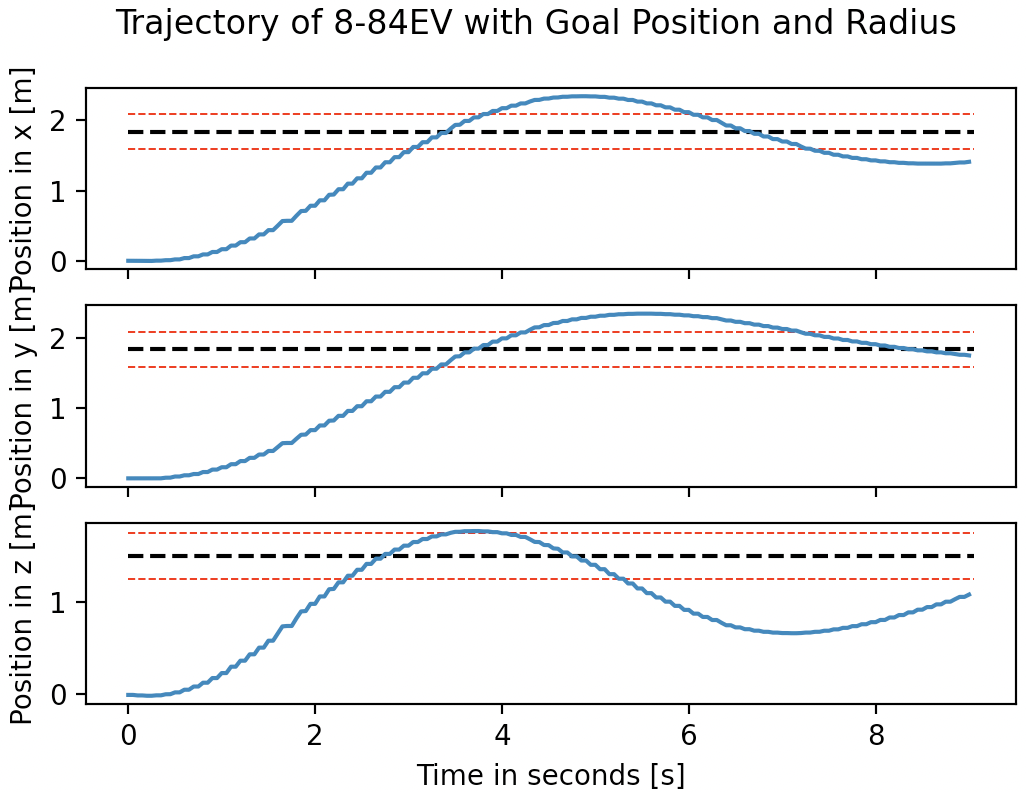
\includegraphics[width=\textwidth]{figures/5_/Testing/ppo_test_884EV2.png}
         \caption{Trajectory of 8-84EV, decomposed in $xyz$.}
         \label{fig:testing_ppo884EV2}
     \end{subfigure} 
     \hfill \\[1mm]
    \begin{subfigure}[b]{0.48\textwidth}
         \centering
         \captionsetup{justification=centering}
         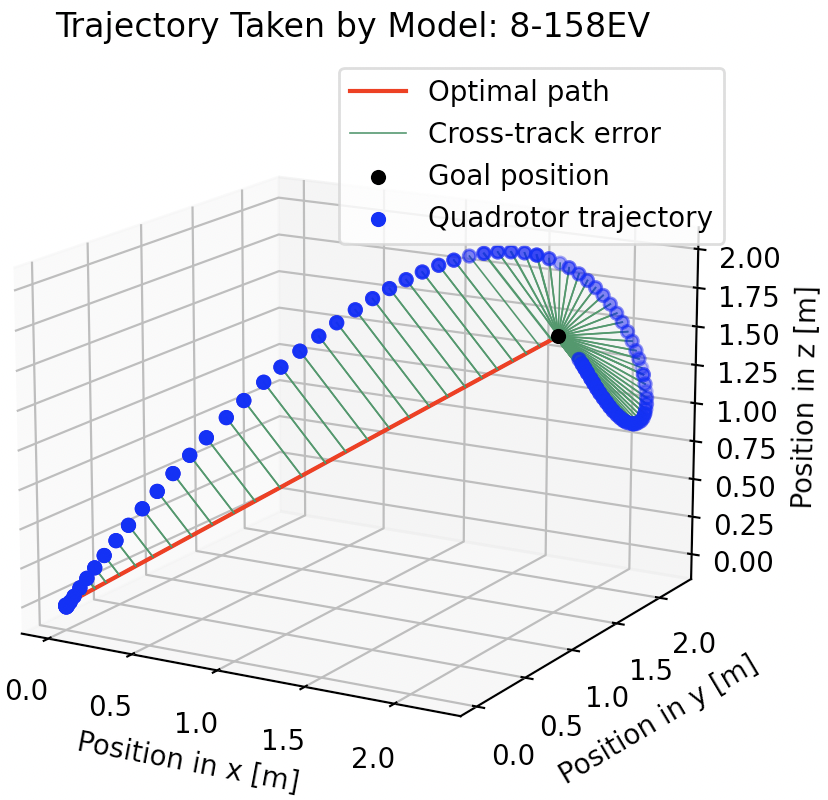
\includegraphics[width=\textwidth]{figures/5_/Testing/ppo_test_8158EV1.png}
         \caption{Trajectory of 8-158EV.}
         \label{fig:testing_ppo8158EV1}
     \end{subfigure} 
     \hfill 
     \begin{subfigure}[b]{0.49\textwidth}
         \centering
         \captionsetup{justification=centering}
         \includegraphics[width=\textwidth]{figures/5_/Testing/ppo_test_8158EV2.png}
         \caption{Trajectory of 8-158EV, decomposed in $xyz$.}
         \label{fig:testing_ppo8158EV2}
     \end{subfigure} 
     \hfill \\[1mm]
    \begin{subfigure}[b]{0.48\textwidth}
         \centering
         \captionsetup{justification=centering}
         \includegraphics[width=\textwidth]{figures/5_/Testing/ppo_test_optimal1.png}
         \caption{Trajectory of Optimal.}
         \label{fig:testing_ppoOptimal1}
     \end{subfigure} 
     \hfill 
     \begin{subfigure}[b]{0.49\textwidth}
         \centering
         \captionsetup{justification=centering}
         \includegraphics[width=\textwidth]{figures/5_/Testing/ppo_test_optimal2.png}
         \caption{Trajectory of Optimal, decomposed in $xyz$.}
         \label{fig:testing_ppoOptimal2}
     \end{subfigure}
    \captionsetup{justification=centering}
    \caption{Test run no. 100 for the 8-84EV, 8-158EV and Optimal PPO models.}
     \label{fig:5_testing_PPO}
\end{figure}
To look into detail of the behaviour of the PPO models, the trajectories for models 8-84EV, 8-158EV and Optimal are shown in \cref{fig:5_testing_PPO}.
Comparing the trajectories of the first two models we see that the 8-158EV model is just about able to reach the goal state at 8 seconds while the 8-84EV model is not. In addition, we see that both models overshoot the goal significantly along the $z$-axis, but is only slightly underdamped in $x$ and $y$. This makes sense from the reward function, where the $z$-term is weighted more than $x$ and $y$, such that the agent wishes to minimise this as fast as possible and perhaps judges overshoots as acceptable.

Moreover, the run no. 100 of model \six is very representative of the average run, having a return of -1.0372 and an RMSE of 0.03679. In contrast, run no. 100 of model \eleven is better than average, with a return of 0.1300 and an RMSE of 0.03861. Thus, both flights are very close in terms of RMSE, but model 8-158EV was much better at exploiting the reward function.

Lastly, for the Optimal model, we see that it reaches the goal with an optimal trajectory in just 2.5 seconds. We observe that there is no oscillatory behaviour, but instead a critically damped response, which shows that the agent has mastered the navigation task. 

\subsubsection{Robustness Test with $\pm10\%$ Mass}
\label{sec:5_ppo_robustnessTests}
Finally, to conclude the PPO tests we will assess the robustness of our best models. From experience in DDPG, it was decided that more time should be given to the models since the model performances were relatively lower. Thus, an extra 5 seconds was added to the timer such that the total time for each episode was 14 seconds. By running the same test with $\pm10\%$ mass and extra time, the results in \cref{table:5_PPO_robustnesstests} were achieved. 
\begin{table}[hbt]
    \centering
    \begin{tabular}{||M{2.3cm}||M{2.5cm}|M{2.5cm}|M{2.5cm}||}
    \hline
    Model & Goal Rate & Average Return & Average RMSE \\\hline\hline
         \textbf{+10\% Mass} &           &            &          \\\hline
8-84EV & 0     &  -2.8492   &  0.0750 \\\hline
8-158EV & 3      & -1.7590     & 0.0495    \\\hline
Optimal & 3      & -0.6705     & 0.0160   \\\hline\hline
         \textbf{-10\% Mass} &           &            &          \\\hline
8-84EV &   0     & -70.8971   &   0.3449  \\\hline
8-158EV &   0    &  -26.8076   &  0.2448 \\\hline
Optimal &   100    &  0.4636   & 0.0404  \\\hline
    \end{tabular}
    \caption{The robustness test results for the PPO models, averaged over 100 episodes. Note that 5 seconds extra was allocated to each episode.}
    \label{table:5_PPO_robustnesstests}
\end{table}
From this table, we see that that model \six struggles the most with these tests, with the being the most negatively impacted for both cases. Further, we can observe from the average RMSE that the +10\% mass case does not affect the trajectory of the quadrotor to a large degree, where models \ten and Optimal have roughly the same RMSEs as without any changes to mass. In the -10\% case, we see that the average RMSE for \ten is significantly worsened, yet the Optimal is not.  

As for the return and goal rate, model \ten struggles in both the +10\% case and -10\% case, with a significant drop in performance. We see that the Optimal model also struggles in the +10\% case but surprisingly manages a 100\% goal rate in the -10\% case.

Looking at Figures \ref{fig:5_testing_robust+10_PPO} and \ref{fig:5_testing_robust-10_PPO}, we observe a behaviour that is reflected in \cref{table:5_PPO_robustnesstests}. From these figures, it is also clear why there is such a low average return and high RMSE for models \six and \ten in the -10\% mass case. The main effect of added mass in the quadrotor results in the quadrotor is that the agent is unable to regulate its height to the goal position. As for its lateral positions, all models do relatively well, staying well within $\pm 1$m from the goal. In contrast, the -10\% mass case causes a drastic overshoot along all axes for models \six and 8-158EV, essentially amplifying the behaviour seen in \cref{fig:5_testing_PPO}. 
Through these examples, we can also confirm that model \ten outperforms model 8-84EV as it was able to maintain a trajectory closer to goal in both mass cases.

An interesting observation for both these models in the +10\% mass case is that both models display an oscillatory accelerate-brake behaviour in the $z$-position despite being nowhere near the goal. This is unexpected, as we should expect that the oscillation occurs around the goal position rather than under it. Thus, we will discuss this more in detail in Section \ref{sec:6_behaviour_robustnessTest_pm10}.

Lastly, for the Optimal model, we can see it was not able reach the goal in the +10\% mass case for the same reason as for the other models, because it was unable to regulate its height to the goal position. On the other hand, it is quite easily able to regulate its height in the -10\% mass case, with only a slight initial overshoot in the $z$-position. However, we can also see that values in \cref{table:5_PPO_robustnesstests} are quite unrepresentative of the Optimal model performance, since it portrays a much worse performance in the +10\% mass case compared to what is actually observed.
\begin{figure}[H]
     \centering
     \begin{subfigure}[b]{0.48\textwidth}
         \centering
         \captionsetup{justification=centering}
         \includegraphics[width=\textwidth]{figures/5_/Testing/ppo_test_robust+10-884EV1.png}
         \caption{Trajectory of 8-84EV +10\% Mass.}
         \label{fig:testing_robust+10_ppo884EV1}
     \end{subfigure} 
     \hfill 
    \begin{subfigure}[b]{0.49\textwidth}
         \centering
         \captionsetup{justification=centering}
         \includegraphics[width=\textwidth]{figures/5_/Testing/ppo_test_robust+10-884EV2.png}
         \caption{Trajectory of 8-84EV +10\% Mass, decomposed in $x$, $y$, $z$.}
         \label{fig:testing_robust+10_ppo884EV2}
     \end{subfigure} 
     \hfill \\[1mm]
    \begin{subfigure}[b]{0.48\textwidth}
         \centering
         \captionsetup{justification=centering}
         \includegraphics[width=\textwidth]{figures/5_/Testing/ppo_test_robust+10-8158EV1.png}
         \caption{Trajectory of 8-158EV +10\% Mass.}
         \label{fig:testing_robust+10_ppo8158EV1}
     \end{subfigure} 
     \hfill 
     \begin{subfigure}[b]{0.49\textwidth}
         \centering
         \captionsetup{justification=centering}
         \includegraphics[width=\textwidth]{figures/5_/Testing/ppo_test_robust+10-8158EV2.png}
         \caption{Trajectory of 8-158EV +10\% Mass, decomposed in $x$, $y$, $z$.}
         \label{fig:testing_robust+10_ppo8158EV2}
     \end{subfigure} 
     \hfill \\[1mm]
    \begin{subfigure}[b]{0.48\textwidth}
         \centering
         \captionsetup{justification=centering}
         \includegraphics[width=\textwidth]{figures/5_/Testing/ppo_test_robust+10-Optimal1.png}
         \caption{Trajectory of Optimal +10\% Mass.}
         \label{fig:testing_robust+10_ppoOptimal1}
     \end{subfigure} 
     \hfill 
     \begin{subfigure}[b]{0.49\textwidth}
         \centering
         \captionsetup{justification=centering}
         \includegraphics[width=\textwidth]{figures/5_/Testing/ppo_test_robust+10-Optimal2.png}
         \caption{Trajectory of Optimal +10\% Mass, decomposed in $x$, $y$, $z$.}
         \label{fig:testing_robust+10_ppoOptimal2}
     \end{subfigure}
    \captionsetup{justification=centering}
    \caption{Robustness test run no. 100 +10\% mass for 8-84EV, 8-158EV and Optimal PPO models.}
     \label{fig:5_testing_robust+10_PPO}
\end{figure}

\begin{figure}[H]
     \centering
     \begin{subfigure}[b]{0.48\textwidth}
         \centering
         \captionsetup{justification=centering}
         \includegraphics[width=\textwidth]{figures/5_/Testing/ppo_test_robust-10-884EV1.png}
         \caption{Trajectory of 8-84EV -10\% Mass.}
         \label{fig:testing_robust-10_ppo884EV1}
     \end{subfigure} 
     \hfill 
    \begin{subfigure}[b]{0.49\textwidth}
         \centering
         \captionsetup{justification=centering}
         \includegraphics[width=\textwidth]{figures/5_/Testing/ppo_test_robust-10-884EV2.png}
         \caption{Trajectory of 8-84EV -10\% Mass, decomposed in $x$, $y$, $z$.}
         \label{fig:testing_robust-10_ppo884EV2}
     \end{subfigure} 
     \hfill \\[1mm]
    \begin{subfigure}[b]{0.48\textwidth}
         \centering
         \captionsetup{justification=centering}
         \includegraphics[width=\textwidth]{figures/5_/Testing/ppo_test_robust-10-8158EV1.png}
         \caption{Trajectory of 8-158EV -10\% Mass.}
         \label{fig:testing_robust-10_ppo8158EV1}
     \end{subfigure} 
     \hfill 
     \begin{subfigure}[b]{0.49\textwidth}
         \centering
         \captionsetup{justification=centering}
         \includegraphics[width=\textwidth]{figures/5_/Testing/ppo_test_robust-10-8158EV2.png}
         \caption{Trajectory of 8-158EV -10\% Mass, decomposed in $x$, $y$, $z$.}
         \label{fig:testing_robust-10_ppo8158EV2}
     \end{subfigure} 
     \hfill \\[1mm]
    \begin{subfigure}[b]{0.48\textwidth}
         \centering
         \captionsetup{justification=centering}
         \includegraphics[width=\textwidth]{figures/5_/Testing/ppo_test_robust-10-Optimal1.png}
         \caption{Trajectory of Optimal -10\% Mass.}
         \label{fig:testing_robust-10_ppoOptimal1}
     \end{subfigure} 
     \hfill 
     \begin{subfigure}[b]{0.49\textwidth}
         \centering
         \captionsetup{justification=centering}
         \includegraphics[width=\textwidth]{figures/5_/Testing/ppo_test_robust-10-Optimal2.png}
         \caption{Trajectory of Optimal -10\% Mass, decomposed in $x$, $y$, $z$.}
         \label{fig:testing_robust-10_ppoOptimal2}
     \end{subfigure}
    \captionsetup{justification=centering}
    \caption{Robustness test run no. 100 -10\% mass for 8-84EV, 8-158EV and Optimal PPO models.}
     \label{fig:5_testing_robust-10_PPO}
\end{figure}


\subsubsection{Brief Summary}
We have seen that the effect of a higher entropy coefficient and value coefficient is beneficial to tested performance, as expected from training. We also confirmed that a batch size of 8000 was good, seen for example in models 4-84EV and 8-84EV.

Otherwise, we obtained some interesting results for the number of optimisation epochs and minibatches, where increasing these improved the chances of reaching the goal, but also led to increased anomalies which lowered the average return and increased RMSE. Thus, we have our most consistent model, 8-84EV, and our most goal-effective model, 8-158EV.

Next, we observed that our Optimal model did not require any hyperparameter tuning and had no troubles in the waypoint navigation task with a perfect 100\% goal rate.

In the robustness tests, we observed that the models \six and \ten struggled only with reaching the goal height in the +10\% mass case but had a drastic overshoots in all axes for the -10\% case. However, the Optimal model was relatively robust, being barely below the goal height in  +10\% mass case and managing a 100\% goal rate in the -10\% case.


\section{DDPG versus PPO}
After a relatively long presentation of results, the best models for DDPG and PPO are summarised in Table \ref{table:5_DDPG_PPO_bestModels}.
\begin{table}[hbt]
    \centering
    \begin{tabular}{||M{2.3cm}||M{2.5cm}|M{2.5cm}|M{2.5cm}||}
    \hline
        Model & Adjusted Goal Rate & Adjusted Avg. Return & Adjusted Avg. RMSE \\\hline\hline
        \textbf{DDPG} &  &   & \\\hline
        Modified & 100 & 0.267 & 0.025   \\\hline\hline
        \textbf{PPO} &   &   & \\\hline
        8-158EV &   85.9  & -0.133 & 0.044 \\\hline
        Optimal &   100  & 0.429 & 0.018 \\\hline
    \end{tabular}
    \caption{The best models for DDPG and PPO, where the results neglect outliers.}
    \label{table:5_DDPG_PPO_bestModels}
\end{table}
This table shows that our Optimal PPO model is the best model overall, which can be further confirmed by comparing its trajectory in Figure \ref{fig:testing_ppoOptimal2} to Modified's trajectory in \cref{fig:testing_ddpgModified2}. Next, DDPG's Modified model easily outperforms model 8-158EV, which has a significantly poorer performance compared to the two best models. 

In addition, we have seen that the PPO models are much quicker to train compared to the DDPG models, taking on average about a third of the total DDPG time to peak performance. This being said, the yield on the additional training time does pay off, resulting in overwhelming success in training for DDPG compared to PPO. The reason for this was that models for DDPG converge to global optima, while PPO models approach some local optima before diverging. The reasons for this will be discussed in Section \ref{sec:6_underperformance_divergence_PPO}. 

The success in training for DDPG was also seen through its test results, with the Original and Modified models dominating PPO in terms of average return and goal rates, and similar in terms of RMSE with PPO's most consistent model, 8-84EV. The reason for this is due to the local optimum strategy of the PPO models -- a trajectory that overshoots the goal height and doing some loop in order to reach the goal -- compared to the direct, globally optimum approach in the DDPG models.

For the robustness tests, the Modified model performed better in the +10\% mass case compared to the PPO models, but surprisingly performed worse than model 8-158EV in the -10\% mass case. For this situation, the overshoot caused by the lower mass was manageable by the PPO loop strategy, while the DDPG model could not adapt in the unfamiliar state space.

However, the wildcard performance of PPO's Optimal model is a testament to the potential of PPO. This model was in all regards optimal, being relatively exceptional in the robustness tests compared to the other models and the only model capable of reaching the goal in the -10\% case, let alone with a 100\% goal rate. As such, from the results in this project, we can conclude that training a DDPG agent is overall easier and more stable, while the potential performance of a PPO agent is unmatched.


\chapter{Discussion}
\label{chap:discussion}
\begin{comment}

Combine with results? why not what part.

Look into what we observed, did we get expected results based on the theory? Why? what limitations did we have for testing? Was there anything weird? What does the theory say we should expect vs. what we saw? 
Sample efficiency, convergence guarantees, changing hyperparameters, actor loss reflected in critic for ppo, the gradient magnitude and divergence, the solution space, the stages of convergence, local optima.
What does the best result say about the algorithm, our reward structure, and structure of experiment? Why did one algorithm outperform the other -- was it expected? Lucky? How did we obtain our best model and how does it reflect in the training and performance. 

Start with DDPG internal discussion, then PPO, then compare the differences between the two. Can we reach a conclusion? Under what assumptions? How critical are we to our experimental setup? 

If time, how could we improve our tests, what would be interesting to find out? 
Show some experiments that verify our thoughts, why it didn't work or why it did. Not enough time, tuning the reward, changing episode structure.

Hyperparameters are NN design parameters that generally affect the optimisation process of the network and ultimately the performance of the model. 
\end{comment}

\section{Size of the Neural Network and Replay Buffer in DDPG}
\label{sec:6_sizeof_NN}

From the training results of DDPG shown in Section \ref{sec:5_ddpg_training}, we saw that increasing the network size significantly was beneficial when compared to the Previous NTNU model, but not when compared to the Modified one. To look into why, we first need to understand this hyperparameter.

So initially, the result based on the network size was unexpected. Rather, what we expected was a something similar to for example deep learning, where we can often just increase the complexity of our model and expect better results in for example, image classification. This is because the model should be able to understand the input space better. To go a bit more into detail, the size of a NN generally correlates to its \textit{generalisation potential}. The greater the number of neurons per layer (width) or the greater the number of hidden layers (depth), there is an exponentially increasing number of parameters that can be used to parametrise the function. 
The idea is that when a NN receives increasingly complex data as input, the NN should be large enough such that it is able to ``understand'' the distribution of the input space or be able to extract higher-level information (features) through the hidden layers of the network \cite{DLUnipd}. The mechanics within NNs are relatively poorly understood however \cite{XAI}, though there is emerging research that focuses on establishing NN size design laws, such as \textit{the law of robustness} in for example \cite{bubeck2021aLawOfRobustness}.
The trade-off when increasing the size of the network, however, is that the length of training is increased as there is a need to calculate many more gradients (in backpropagation) for the increased number of parameters.  

Yet, we saw that despite having a longer training time, the performance was still not matching that of the Modified model. Furthermore, as this project was conducted, we found that our input space was quite simple in comparison to other papers, such as in \cite{song2021droneRacing} which had an input dimension of 18. Thus, our view on the size of the network greatly resonates with \cite{ControlofQuadrotorRL}, who states \textit{neural networks are quite versatile and can cope with variety of problems with a single structure.}

So, in my opinion, there is one main explanation for the difference in performance: the effect caused by the other  hyperparameter which differs among the two models, namely the \textit{size of the replay buffer R}.

Since DDPG learns off-policy by sampling experiences from its replay buffer, the agents behaviour correlates with experiences it has in its replay buffer. So, the idea is that if there are a lot of good-action experiences in the relay buffer, we expect DDPG to learn this behaviour quite quickly since it has a good probability of sampling these experiences when sampling uniformly across the buffer. If there are only a with few good-action experiences, we imagine that DDPG will struggle to learn what works well since these experiences are less likely to be sampled. Also, as training proceeds, we do expect that the agent does improve, such that the experiences stored later in the replay buffer are less random but rather good actions with more ``conviction''. So since the replay buffer is a sliding window of the agent's last experiences, we expect that a small replay buffer to only hold relatively good new experiences, while large ones contain many old ``bad'' actions. 

As a result, the size of the replay buffer thus influences the \textit{speed of learning} in DDPG, such that we expect agents with smaller replay buffers to train faster. Yet, we cannot have a too small replay buffer for two reasons: we do not wish to converge to some local optima, and we need i.i.d. samples as described in Section \ref{subsec:DDPG_Innovations}. So, there is therefore also a trade-off with stability.
Thus, the use of a larger replay buffer in the Original model could be an explanation of why it was outperformed by the Modified model -- primarily because it was learning slower. So, for further work, this can be confirmed experimentally.

\section{Learning Rate and Stability in DDPG}
\label{sec:6_learningrate_DDPG}
The learning rate for DDPG proved to have a profound effect in the learning of the DDPG models, being the only hyperparameter separating the best Modified model and the worst Previous NTNU model.

This was a good validation of the theory behind the learning rate, which is that increasing the learning rate can allow networks to converge to better performances, by essentially not getting ``stuck'' in the optimisation space. This is quite certainly the reason why the Previous NTNU model does not improve and maintained an almost constant average return, despite not having an ``optimal'' behaviour.

Yet, the extent of improvement by simply increasing the learning rate was quite unexpected since increasing the learning rate too high could lead to convergence in a local optima or instability due to large gradient updates. The reasons why this did not happen could be justified with two related reasons. The first could be because the learning rate in the Previous NTNU model was unnecessarily low, while the second could be due to stable design of DDPG through its use of target networks. This makes sense because after every large update, due to the soft update rule, the target NNs only change with a weight $\tau = 0.001$, which counteracts the initially large update. As a result, this also explains why training times are long in comparison to PPO, where the relatively fast Modified model required more than 800 epochs ($\approx$10 hours) for the critic network to converge.

\section{Size of the Trajectory and Learning Rate in PPO}
\label{sec:6_sizeof_trajectory}
Quite early in the project, the idea of increasing the length of the trajectory seemed like a good idea. An idea was that, similarly to the effect of the DDPG's replay buffer, PPO's trajectory $T$ served as a type of on-policy replay buffer. This thought was further supported by the fact that agents learning continuous robotic tasks often required more experiences to reflect the larger state and action spaces, which can be seen in the Appendices of \cite{PPO} and \cite{ppoOnDota2020}. 

The underlying theory is that increasing the batch size should improve stability. This is because the gradients calculated are averaged across a larger number of experiences, which reduces noise and variance in gradient updates \cite{batchsizeInvariance}.
By changing the batch size from 2000 to 4000 (though not seen in this project), we achieved much better performances overall which confirmed our initial theory. From Section \ref{sec:5_PPO}, we saw a further increase of the batch size from 4000 to 8000 generally provides good results, and is recommended if an increase the number of optimisation epochs and number of minibatches is desired.

In \cite{batchsizeInvariance}, it is mentioned that increasing the batch size by a factor 2 should be equivalent to reducing the Adam learning rate by a $\sqrt{2}$. This was tested by reducing the learning rate from 3e-4 to 2e-4 with a model 4-44, which produced surprisingly poor results compared to doubling the batch size in 8-44. Anyways, this was still explored with $\alpha$ lowered to 1e-5 in steps, but with similar poor training. Hence, the claim by \cite{DeepLearningBook}, and reiterated in \cite{batchsizeInvariance}, that ``the most important hyperparameter is the learning rate'', could not be verified in the same way as for DDPG, with the reason for this being uncertain. Thus, further testing in along this path was abandoned and efforts were focused on the varying the batch size, consolidated by \cite{dontdecayLRIncreaseBatch}. Nonetheless, as further work, a deeper analysis into why we did not manage to utilise the learning rate properly should be made and more testing of the PPO learning rate should be done.


\section{Speed of Learning and Anomaly Runs in PPO}
\label{sec:6_speed_of_learning_anomaly_runs}
There were a variety of hyperparameters that influenced the training speed in PPO; these were the number of optimisation epochs, number of minibatches, value coefficient and, to some extent, the entropy coefficient. 

One rather unexpected effect of increasing the speed of learning, particularly in the number of optimisation epochs and number of minibatches, was that there was an increased number of anomaly runs -- runs with dramatically poor performance as a result of the agent flying into the distance. The frequency of these inconsistent runs increased simultaneously as the non-anomaly (adjusted) performance improved.

An explanation for this follows from the on-policy learning of PPO. Since PPO learns through gaining experience from its recent and proximal (close) policy, the actions taken from a known state-space should be relatively similar. This means that when making larger updates, through an increased number of gradient updates, sort of enforces PPO to commit to its idea of a ``good'' behaviour. However, given that PPO is on-policy, this means that future experiences sampled from the environment are less exploratory in nature, which potentially makes PPO commit to a locally optimal solution as it most likely had no time to find an alternative. These larger updates can be thought of as going all-in on a locally optimal solution, while a more conservative model, such as 8-84EV, requires a longer time to reach this same point, but gathers more experience as a result.

Therefore, in the results for the PPO tests, a possible theory is that the simple waypoint navigation task is essentially a known state-space for these PPO models, such that a locally optimal solution in a fast-trained model outperforms a conservative model which does not commit to the same local optimum to the same extent. 
This can be the reason why the fastest models, such as 8-158EV, also have the highest average returns in training.
However, in the random event that the fast-trained agent ends up in some unknown state, we see that the it does not have the experience to handle this and flies off, resulting in many anomaly runs with a very negative average return. On the contrary, for the conservative model 8-84EV, we saw in \cref{table:5_PPO_test_bestModels} that it essentially had no anomaly runs, which suggests that this random anomaly event was very unlikely, which could be explained by its increased experience in training. 



\section{Underperformance and Divergence in PPO}
\label{sec:6_underperformance_divergence_PPO}

One of the biggest unmet -- and perhaps, in hindsight, naive -- expectations was that training a PPO agent should be an easy task. The reason for this was largely due the benefits of on-policy methods, which includes faster training by, ``ignoring uninteresting parts of the space'' and ``faster initial planning'' \cite{suttonAndBartoBook}, better data-efficiency \cite{PPO}, but also because of ``stronger convergence results'' when sampling on-policy \cite{suttonAndBartoBook} and the supposed, ``guaranteed monotonic improvement'' from trust-region based policy optimisation \cite{TRPO}.

\subsection{Understanding the Local Optima}
One of the reasons why this has been difficult is natural: hyperparameter tuning in deep reinforcement learning is highly sensitive \cite{selftuningAC}. This is due to the fact that reinforcement learning tasks has often a complicated state-action space, along with a few loss functions in e.g. actor-critics, that results in a very complex optimisation space. 

A prevalent example of this has been in the existence of a local optima for all PPO models. This local optima proved to be a satisfactory temporary solution for the PPO agents, but also led to an immediate divergence in training. To get an intuitive understanding of this, the path to the local optima represented where the agent had ``figured out'' that accelerating to the goal resulting in high rewards. However, as it learned to reach the goal faster and faster, it had not yet learned to brake properly, such that after reaching its peak average return, the models were continuously overshooting the goal and receiving very negative rewards. From a state-space perspective, this local optima makes sense too. Initially, all that should be learned is to point the acceleration vector $\a_t$ in the direction of the position vector $\p_t$. However, the next step for the agent is perhaps more unintuitive for the agent, which is to point $\a_t$ in the opposite direction of $\p_t$, when $\p_t$ is small and $\v_t$ is large. 

So this is an explanation for why we observed such a significant drop in the average return after each peak in the training plots. However, a natural follow-up would be to ask \textit{why did there have to be a divergence?} In other words, why did we not see a monotonic improvement during training, like in for example the Optimal model? 

\subsection{High Actor Loss at the Local Optima}
If we consider the training plots for PPO again, we noticed a strange observation in the actor loss plots: that the actor loss was increasing before each peak in average return, though at the same time, the average return was increasing and the critic loss decreasing. 
If we consider again what the actor loss represented, a large positive value signified that the advantage $\hat{A}_t$ was very negative, such that the agent was performing very poorly. So looking at Equation \eqref{3_5_advantage}, if the critic value estimate $V_{\bt}(s)$ was quite accurate, this would mean that the agent was simply choosing actions that resulted in a very poor negative $Q(s,a)$. 
So how can we explain consistently poorer agent actions, when we observe an increasing average return? 

Well, a possible justification, which was not apparent in the training plots, could be made from the existence of these \textit{anomaly runs} that we saw during testing. And as explained in \ref{sec:6_speed_of_learning_anomaly_runs}, these were increasingly common in the fastest models, despite the average return increasing. 
So we can imagine that as the agents approach their local optima, overshooting the goal became more common, and for each overshot there was a chance of it becoming an anomaly run.
Therefore, in a batch of 4000 or 8000 episodes, we can expect that the very negative rewards received from these anomaly runs were then resulting in very negative advantage estimates and spikes in the actor loss.

\subsection{Large Updates in the Optimisation Space}
Now, to go back to the question of divergence, we can try to understand the role of large updates in the optimisation space. The idea of performing gradient ascent in the actor-objective-function solution space can be thought of as hiking up a ridge between many tall mountains. 

We can then imagine that when approaching a peak (perhaps a sharp maxima), the ridge becomes thinner and its sides become steeper. In this scenario, it is intuitive that we wish to take smaller steps, as to not fall down the mountain ridge. 
However, as explained in the the previous section, what happens is the opposite: the actor loss becomes increasingly high which translates to large gradient updates -- large steps near our mountain peak. So naturally, our training process is unstable and making too big a step and falling off the ridge is inevitable given the very high actor loss near the local optima.

\subsection{Possible Improvements}
\label{subsec:6_possible_improvements}
From this discussion, it seems almost clear that attempting a much lower learning rate should be the key achieving a good PPO performance. But, as already discussed, this was attempted with no success. Also, after the Optimal PPO model was achieved with a model 4-44, it seemed like we were in the right parameter space to achieve good PPO performances and we did not need to lower the learning rate. 

Alternatively, it can be argued that training more conservative models, such as 8-84EV, rather than fast models 8-158EV, is beneficial because of the lack of anomaly runs. Though, as we observe in \cref{fig:5_training_ppo_bestModels}, even when training a model 4-44 resulted in divergence, despite having lower actor losses than 8-84EV. 

What we can conclude from this, is that the tuning the many hyperparameters of PPO is complicated and excessive tuning will not guarantee an optimal solution. Furthermore, due to the complex optimisation space and the existence of the local optima -- the lack of exploration in PPO due to the nature of its on-policy sampling presents a major problem. As we have seen, no matter how drastic hyperparameters are tuned, we always converge to the same local optima and diverge shortly after.

Therefore, there are three major improvements that can be made to this implementation. 
\begin{enumerate}
    \item Reduce the rate of learning by finding out how to reduce the learning rate properly. Too much focus was put into reaching a good solution early on, which constantly led to the convergence of a local optimum.
    \item Due to the complex optimisation space, a lucky initialisation can play a large role in finding a globally optimal solution, seen for example in the Optimal model. Thus, parallel initialisation would be a large step in the right direction.
    \item Since we have such a predominant local optima when training our PPO models, another consideration is to alter the implementation of this experiment slightly, such it is easier to find a globally optimal solution.
\end{enumerate}
As an example of altering the implementation, one could for example add 5 seconds extra to episodes and remove the termination condition when reaching the goal. This simple change should the local optima, since the models have plenty of time to reach the goal state and will not learn to accelerate excessively to the goal. 
By testing this hypothesis, the models in Table \ref{table:6_experimental} were used. Analysing their performance is out of the scope of this project, but the hypothesis was verified, where a goal rate of 99\% and RMSE of 0.0151 was achieved for model 14, and a rate of 94\% and RMSE of 0.0498 was achieved for 13.
\begin{table}[hbt]
    \centering
    \resizebox{\textwidth}{!}{%
    \begin{tabular}{||M{0.6cm}|M{2cm}||M{1.8cm}|M{1.8cm}|M{1.7cm}|M{1.4cm}|M{1.4cm}|M{1.4cm}||}    \hline
ID & Model    & Trajectory, T & Learning rate $\alpha$  & N. opt. epochs, K & N. minibatches & Ent. coef. $c_2$ & VF coef. $c_1$  \\ \hline\hline
13 & ER8-44EV & 8000          & 3,00E-04                      & 4                 & 4 & 1              & 0,01              \\ \hline
14 & ER8-88EV & 8000          & 3,00E-04                      & 8                 & 8 & 1              & 0,01              \\ \hline
    \end{tabular}
    }
    \caption{Experimental models with extra Time and no reward limit when reaching goal.}
    \label{table:6_experimental}
\end{table}

\section{Agent Behaviour with $\pm10\%$ Mass}
\label{sec:6_behaviour_robustnessTest_pm10}

In Figures \ref{fig:ddpg_test_robust}, \ref{fig:5_testing_robust+10_PPO} and \ref{fig:5_testing_robust-10_PPO} of the DDPG and PPO robustness test, we observed a clear decrease in performances when the quadrotor weight was altered. This was in contrast to our initial guess that a $\pm 10\%$ mass difference was quite a conservative robustness test. 

In my opinion, it is not exactly clear why changing mass should cause an effect in the agent performance. I would argue that since the agent is commanding accelerations to guide the quadrotor motion, what we expect it to learn is simply just a kinematic relationship -- the relationship between acceleration, velocity and position. However, this relationship, by definition, is independent of the forces acting on the quadrotor, or its kinetics. To take a simple example, the gravitational acceleration of Earth is defined as 9.81ms$^{-2}$. This acceleration is completely irrespective of mass, such that a 1kg or 10kg mass will accelerate identically at 9.81ms$^{-2}$ towards Earth in a vacuum. Following the same idea, if the quadrotor has learned to map positions and velocities to accelerations, the effect of the commanded acceleration on a quadrotor of mass 1kg or 10kg should be identical. 

Yet, this theory does not fit our observations. We see clearly that the mass does have an effect on the quadrotor behaviour, despite the agent commanding acceleration. A natural direction could be to then discuss possible reasons for why the actual accelerations are not matching the commanded ones. First, we can look at is the physical relationship between acceleration and mass. 
Essentially, the motion of the quadrotor is caused by the generalised forces acting along the $xyz$-axes, known through Newton's second law of motion $\a = \boldsymbol{f}/m$. This relationship matches the observed behaviour, where the mass acts like a \textit{gain}, such that the same commanded accelerations are mapped to smaller forces in the $+10\%$ mass case and larger forces for $-10\%$. 
For this to be true, it means that somewhere in the control loop, there exists a fixed mapping between acceleration and generalised force which does not get updated when there is a change in mass. Based on the rigid-body dynamics in Section \ref{sec:4_2_dynamics}, we know this is not true. Instead, the underlying PD-controller is designed such that the commanded accelerations are translated into desired pitch and roll angles, $\theta_d$ and $\phi_d$. Then, the PD-controller should generate the thrusts to ensure $\theta = \theta_d$ and $\phi = \phi_d$ such that we achieve the accelerations we desire. But, in equations \eqref{4_2_udot} and \eqref{4_2_vdot}, we see that there is in fact another mapping which includes the mass -- the mapping of desired accelerations to the pitch and roll angles. From these equations, we understand that if the mass of the quadrotor should change we expect that the desired pitch and roll angles should also change: a fixed acceleration should map to a larger pitch and roll angle in the $+10\%$ mass case, and the same acceleration should map to a smaller pitch and roll angle in the $-10\%$ case.
So if the mass of the quadrotor is changed directly in the simulator, but not registered in the controller, this could lead to accelerations which are not planned by the agent, which is a possible source of error.

This theory is supported by the -10\% case in Figures \ref{fig:ddpg_test_robust} and \ref{fig:5_testing_robust-10_PPO}, where we see that the quadrotor accelerates excessively in all axes, overshooting the goal position. If we consider the +10\% mass case, we see that this theory also holds to some extent. We observe in Figures \ref{fig:ddpg_test_robust} and \ref{fig:5_testing_robust+10_PPO} that generally takes a bit longer time to reach the goal position in all axes, for example taking less 3 seconds in all axes compared to about 4 seconds in average when 10\% mass was added for DDPG.
Furthermore in \cref{fig:5_testing_robust+10_PPO}, we observed that the PPO models exhibited some oscillatory behaviour along $z$, despite flying quite below the goal height. To explain this, we first have to note an interesting observation in the initialisation of the simulator.
\begin{figure}[H]
     \centering
     \begin{subfigure}[b]{0.49\textwidth}
         \centering
         \captionsetup{justification=centering}
         \includegraphics[width=0.72\textwidth]{figures/6_/quadrotor+10.png}
         \caption{Position of quadrotor when initialised with +10\% mass.}
         \label{fig:6_quadrotor+10}
     \end{subfigure} 
     \hfill 
    \begin{subfigure}[b]{0.49\textwidth}
         \centering
         \captionsetup{justification=centering}
         \includegraphics[width=0.8\textwidth]{figures/6_/quadrotor-10.png}
         \caption{Position of quadrotor when initialised with -10\% mass.}
         \label{fig:6_quadrotor-10}
     \end{subfigure} 
    \caption{The change in initialised position when altering the weight of the quadrotor.}
    \label{fig:6_quadrotor_mass}
\end{figure}
In \cref{fig:6_quadrotor_mass}, we observe that there is significant height difference in the initialisation position of the quadrotor. We see that when the mass is increased, there is a large negative constant deviation from the desired height, while for the -10\% mass case we see a large positive constant deviation from the desired height.
Knowing that the underlying controller for position is a PD-controller, we can therefore conclude that the is some sort of feedforward gravity term which does not get updated when the mass is changed, resulting in the constant deviations. Thus, in \cref{fig:5_testing_robust+10_PPO}, the reason the agent is not able to reach the goal is not because it is not accelerating upwards, but because the underlying PD controller is not able to regulate its height due to the unbalanced gravitational force.

To explain the oscillatory behaviour in the figure, we can guess that  it occurs because the agent thinks that it will reach the goal with some certain acceleration, and once it reads a change in velocities, it stops to not overshoot. However, since the PD controller is not compensating for the gravity term, the quadrotor instead decelerates due to gravity and starts falling down, such that the agent is constantly accelerating upwards and not reaching goal.

Another reason for why there could be a discrepancy between the actual and commanded accelerations could be in the bandwidth separation between the agent's choice of actions and the control bandwidth of the system. For a PD-controlled quadrotor, its closed-loop dynamics could be compared to a mass-spring-damper system such as \cite{Fossen2021}:
\begin{align}
    m\Ddot{x} + K_d\Dot{x} + K_p\Tilde{x} &= 0 \\
    \Ddot{x} + 2\zeta\omega_n\Dot{x} + \omega_n^2 &= 0
\end{align}
With this, the relative damping factor and natural frequency of the system is given by:
\begin{equation}
    \zeta = \frac{K_d}{2m\omega_n}, \qquad \omega_n = \sqrt{\frac{K_p}{m}}
\end{equation}
From this, we see quite clearly that the closed-loop frequency of the controller is inversely proportional to the mass. This means that when the mass is altered, the speed (time constant) of the system also changes.
As a result, when the mass of the quadrotor increases, there is a possibility that the PD-controller struggles to keep up with the agent actions, such that the agent behaviour is impaired. This agent-to-controller time-delay due to slow dynamics in the feedback loop could also help to explain why there are low frequency oscillations in \cref{fig:5_testing_robust+10_PPO}, rather than just a constant deviation.
On the contrary, when there is less mass there is a sufficient bandwidth separation so this theory does not apply. Yet, another possible consequence is that a perfectly tuned PD-controller would become underdamped if the mass decreases, which could then lead to an unstable oscillatory system if it the physical quadrotor cannot keep up, which has its own slower time constant.

\chapter{Conclusion}
\label{chap:conclusion}

\begin{comment}
A concise summary of essential information and findings in the project.
\end{comment}

A growing interest in autonomy in today's society has spurred the development of new solutions within guidance, navigation and control of vehicles. Reinforcement learning has emerged as one of the tools capable of solving guidance and control tasks, in light of its success in recent years within the domain of robotic tasks.
In this project, we have studied the use of two reinforcement learning algorithms, DDPG and PPO, as potential guidance systems for a quadrotor.

We have learned that DDPG and PPO are two model-free actor-critic algorithms, capable on handling high-dimensional continuous state and action spaces through the use of NN parametrisations of the actor and critics. However, introduction of NNs as function approximators had its own onset of challenges which were then handled uniquely for DDPG and PPO. 
For DDPG, the instability induced through its function-approximation, bootstrapping and off-policy learning was handled through the introduction of target networks and a replay buffer. Then to optimise its policy, the deterministic policy gradient was used.
For PPO, it introduced a novel clipped surrogate objective, which was used to both optimise its policy, while offering stability and reliability through small updates.

Then, to compare these models, the algorithms were demonstrated on an RMF in Gazebo, where the task was to command acceleration in order to reach a waypoint in 3-dimensional space. The algorithms were studied under the context of hyperparameter testing, where models with different combinations of hyperparameters were trained, tested and evaluated.

From the results, it was proved that DDPG produced consistent performances compared to PPO, though PPO has the best potential performance. Of the models trained, Modified was the best DDPG model while the Optimal model was the best PPO one.
It was further found that DDPG offered a high degree of stability, such that we could achieve improved results by increasing its learning rate and reducing the size of the replay buffer. 
As for PPO, training the agents to an optimal solution proved to be unsuccessful -- with the exception of the Optimal model -- such that the effect of hyperparameters were compared in relation to a local optimum. 
From this we observed that increasing the number of optimisation epochs, number of minibatches and increasing the value function coefficient increased the rate of convergence, though this could only be done if the batch size was increased, where 8000 had the best results. The faster training also proved to have slightly better results in testing and training, but also increased the rate of anomaly runs where the quadrotor flew off into distance. However, in hindsight, it was discussed the speed of training for PPO generally was too high, such that increased anomaly runs and high gradient updates resulted in divergence in training. 

Otherwise, it was discussed that that navigating the complex optimisation space is difficult, such that a lack of exploration in PPO due to its on-policy sampling is a major challenge. Due to this complex optimisation space, a lucky initialisation could thus play a major role in converging to a good result, irregardless of hyperparameter tuning, as exemplified by the Optimal model. So as an improvement to training consistency, changing the implementation was a suggestion, where an idea is to for example add 5 seconds extra to each episode and allow the quadrotor to accumulate goal rewards in a non-terminal goal state.

Lastly, a final comparison was made by testing the robustness of algorithms under a $\pm10\%$ mass change to the quadrotor. It was shown that the only the Optimal model was able to handle this test, performing exceptionally well in relation to all other models. However, this test was suspiciously difficult and after a thorough discussion, the poor performance was not necessarily the fault of the agent but of the underlying PD-controller. Therefore, an alternative robustness test can be proposed as further work.



\begin{comment}

\section{Further work}

For further work, 

D4PG: We also combine this technique with a number of additional, simple improvements such as the use of N-step returns and prioritized experience replay. 

MADDPG: Multi-agent variant

PPO: Released with multi-agent possibility

STAC: Self-tuning AC

\end{comment}

\printbibliography
\appendix
\chapter{Acronyms}
\label{app:acronyms}

\textbf{Q} - Action-value \\[-4mm]

\noindent
\textbf{DQNs} - Deep Q-Networks \\[-4mm]

\noindent
\textbf{DPG} - Deterministic Policy Gradients \\[-4mm]

\noindent
\textbf{DDPG} - Deep Deterministic Policy Gradients \\[-4mm]

\noindent
\textbf{TRPO} - Trust-Region Policy Optimisation \\[-4mm]

\noindent
\textbf{ACER} - Actor-Critic Experience Replay \\[-4mm]

\noindent
\textbf{PPO} - Proximal Policy Optimization \\[-4mm]

\noindent
\textbf{MDPs} - Finite Markov Decision Processes \\[-4mm]

\noindent
\textbf{POMDPs} - Partially Observed Markov Decision Processes \\[-4mm]

\noindent
\textbf{TD} - Temporal difference \\[-4mm]

\noindent
$\boldsymbol{\overline{VE}}$ - Prediction error \\[-4mm]

\noindent
\textbf{SARSA} - State-Action-Reward-State-Action \\[-4mm]

\noindent
\textbf{NNs} - Neural networks \\[-4mm]

\noindent
\textbf{DNNs} - Deep neural networks \\[-4mm]

\noindent
\textbf{CNNs} - Convolutional neural networks \\[-4mm]

\noindent
\textbf{RNNs} - Recurrent neural networks \\[-4mm]

\noindent
\textbf{MLP} - Multi-layer Perceptron \\[-4mm]

\noindent
\textbf{KL} - Kullback-Leibler \\[-4mm]

\noindent
\textbf{MSE} - Mean-squared error \\[-4mm]

\noindent
\textbf{RMSE} - Root-mean-squared error \\[-4mm]

\noindent
\textbf{QP} - Quadratic Programming \\[-4mm]

\noindent
\textbf{PD controller} - Proportional-derivative controller \\[-4mm]

\noindent
\textbf{RMF} - Resilient micro-flyer \\[-4mm]

\noindent
\textbf{MAV} - Micro aerial vehicle \\[-4mm]

\noindent
\textbf{URDF} -  Unified Robotic Description Format \\[-4mm]

\noindent
\textbf{ROS} - Robot Operating System \\[-4mm]




\chapter{Algorithms}
\label{app:algs}

\section{One-step Actor-Critic}
\label{app:algs_ActorCritic}
\begin{algorithm}
\caption{One-step Actor-Critic, from \cite{suttonAndBartoBook}} \label{alg:OneStepActorCritic}
    \begin{algorithmic}[1]
    \State Input: a differentiable policy parameterisation $\pi (a \mid s, \boldsymbol{\theta}$
    \State Input: a differentiable state-value function parameterisation $\hat{v}(s, \boldsymbol{w})$
    \State Parameters: step sizes $\alpha^{\boldsymbol{\theta}} > 0$, $\alpha^{\boldsymbol{w}} > 0$ (learning rates)
    \State Initialize policy parameters $\boldsymbol{\theta} \in \R^{d'}$ and state-value weights $\boldsymbol{w} \in \R^d$
    \For {each episode}
    
        \State Initialize S (first state of episode)
        \State I $\gets$ 1
        
        \While {\text{S is not terminal}}
        
            \State A $\sim \pi ( \dot \mid S, \boldsymbol{\theta})$
            \State Take action A, observe S', R
            \State $\delta \leftarrow R + \gamma \hat{v}(S', \boldsymbol{w}) - \hat{v}(S, \boldsymbol{w})$
            \State $\boldsymbol{w} \leftarrow \boldsymbol{w} + \alpha^{\boldsymbol{w}} \delta \nabla \hat{v}(S, \boldsymbol{w})$
            \State $\boldsymbol{\theta} \leftarrow \boldsymbol{\theta} + \alpha^{\boldsymbol{\theta}} I \delta \nabla \ln \pi (A \mid S, \boldsymbol{\theta})$
            \State $I \leftarrow \gamma I$
            \State $S \leftarrow S'$
        \EndWhile
    \EndFor
    \end{algorithmic}
\end{algorithm}
\noindent
This implementation is taken from the Sutton \& Barto's book \cite{suttonAndBartoBook}.

\newpage
\section{DDPG}
\label{app:algs_DDPG}

\begin{algorithm}
\caption{DDPG, from \cite{DDPG}} \label{alg:DDPG}
\begin{algorithmic}[1]
\State Randomly initialise critic network $Q(s,a | \bt^Q)$ and actor $\mu(s|\bt^\mu)$ with weights $\bt^Q$ and $\bt^\mu$
\State Initialise target network $Q'$ and $\mu'$ with weights $\bt^{Q'} \leftarrow \bt^{Q'}, \bt^{\mu'} \longleftarrow \bt^{\mu'}$  
\State Initialise replay buffer $R$
\For{episode = 1, M}
\State Initialise a random process $\mathcal{N}$ for exploration noise
\State Receive initial observation state $s_1$  %\Comment{This is a comment}

    \For{t = 1, T}
        \State Select action $a_t = \mu(s_t | \bt^{\mu}) + \mathcal{N}_t$ according to the current policy and exploration noise 
        \State Execute action $a_t$ and observe reward $r_t$ and observe new state $s_{t+1}$
        \State Store transition $(s_t, a_t, r_t, s_{t+1})$
        \State Sample a random minibatch of $N$ transitions $(s_t, a_t, r_t, s_{t+1})$ from $R$
        \State Set $y_i = r_i + \gamma Q'(s_{t+1}, \mu'( s_{t+1}| \bt^{\mu'}) \,|\, \bt^{Q'} )$ 
        \State Update critic by minimizing the loss:
        \begin{equation*}
            L = \frac{1}{N} \sum_i (y_i - Q(s_i, a_i \,|\, \bt^Q))^2
        \end{equation*}
        \State Update the actor policy using the sampled policy gradient:
        \begin{equation*}
            \nabla_{\bt^\mu} J \approx \sum_i \nabla_a Q(s, a \,|\, \bt^Q) \,|_{s=s_i, a=\mu(s_i)} \nabla_{\bt^\mu} \mu(s_t | \bt^{\mu}) \,|_{s_i}
        \end{equation*}
        \State Update the target networks:
        \begin{align*}
            \bt^{Q'} &\leftarrow \tau \bt^Q + (1-\tau) \bt^{Q'}  \\
            \bt^{\mu'} &\leftarrow  \tau \bt^\mu + (1-\tau) \bt^{\mu'} 
        \end{align*}
    \EndFor
\EndFor
\end{algorithmic}
\end{algorithm}
\noindent
This implementation is acquired from the original paper \cite{DDPG}.
\newpage

\section{Proximal Policy Optimization}
\label{app:algs_PPO}

\begin{algorithm}
\caption{PPO Actor-Critic style, from \cite{PPO}} \label{alg:PPO_actorCriticStyle}
\begin{algorithmic}[1]
\For {iteration = 1, 2, ...}
    \For{actor = 1, 2, ..., $N$}
        \State Run policy $\pi_{\theta_{old}}$ in environment for $T$ timesteps
        \State Compute advantage estimates $\hat{A}_1 ,..., \hat{A}_T$
    \EndFor
    
    \State Optimize surrogate L with respect to $\theta$, with K epochs and minibatch size $M \leq NT$
    \State $\theta_{old} \leftarrow \theta $
\EndFor
\end{algorithmic}
\end{algorithm}
\noindent
This implementation is acquired from the original paper \cite{PPO}. Note that in our implementation we have $N=1$ actors. \vspace{8mm}

\begin{algorithm}
\caption{PPO-Clip, from \href{https://spinningup.openai.com/en/latest/algorithms/ppo.html}{Spinning Up, OpenAI}} \label{alg:PPO_spinningUp}
\begin{algorithmic}[1]
\State Input: initial policy parameters $\theta_0$, initial value function parameters $\phi_0$
\For {k = 0, 1, 2, ...}
    \State Collect set of trajectories $\mathcal{D}_k = \{\tau_i\}$ by running policy $\pi_k = \pi(\theta_k)$ in the environment.
    \State Compute the return $\hat{R}_t$.
    \State Compute advantage estimates, $\hat{A}_t$ based on the current value function $V_{\phi_k}$
    \State Update the policy by maximizing the PPO-Clip objective:
    \[
    \theta_{k+1} = \arg \max_\theta \frac{1}{|\mathcal{D}_k|T} \sum_{\tau \in \mathcal{D}_k} \sum^{T}_{t=0} \min \left(
    \frac{\pi_\theta (a_t | s_t)}{\pi_{\theta_k} (a_t | s_t)} 
    A^{\pi_{\theta_k}}(s_t, \, a_t), \,\, g(\epsilon, A^{\pi_{\theta_k}}(s_t, \, a_t))
    \right),
    \]
    typically via a stochastic gradient ascent algorithm with Adam.
    \State Fit value function by regression on mean-squared error:
    \[
    \phi_{k+1} = \arg \min_\phi \frac{1}{|\mathcal{D}_k|T} \sum_{\tau \in \mathcal{D}_k} \sum^{T}_{t=0}
    \Big(
    V_\phi (s_t) - \hat{R}_t
    \Big)^2,
    \]
    typically via some stochastic gradient descent algorithm.
\EndFor
\end{algorithmic}
\end{algorithm}

\noindent
Algorithm \ref{alg:PPO_spinningUp} is acquired from OpenAI's Spinning Up documentation:\\
https://spinningup.openai.com/en/latest/algorithms/ppo.html 




\end{document}
